\documentclass[10pt,journal,compsoc]{IEEEtran} %,compsoc

% the package used are listed below
\usepackage{enumerate} %put a number in front of every paragraph
\usepackage{cite} %
\usepackage{amsmath}
\interdisplaylinepenalty=2500
\usepackage{algorithm}
\usepackage{algorithmic}
\usepackage{graphicx}
\usepackage{multirow}
\usepackage{subfigure}
\usepackage{amssymb}
\usepackage[normalem]{ulem}
%\usepackage[maxfloats=25]{morefloats}
\hyphenation{op-tical net-works semi-conduc-tor}

%%% Stuff from Dave
\usepackage{verbatim}
\usepackage{xcolor}
% Dave's comments

\newcounter{DaveCommentCounter}
\setcounter{DaveCommentCounter}{0}
  % Use this version of dpt to have comments produced in-text
\newcommand{\dpt}[1]{
    \stepcounter{DaveCommentCounter}
    \textcolor{blue}{\emph{/** Dave [\arabic{DaveCommentCounter}]: #1 **/}}
}

\newcommand{\rrf}{
    \stepcounter{DaveCommentCounter}
    \textcolor{blue}{\emph{/**Dave [\arabic{DaveCommentCounter}]: NEED REFERENCES **/}}
}

%%% Stuff from Dave

\begin{document}

\title{Dynamic Random Testing of Web Services: \\ A Methodology and Evaluation}


\author{Chang-ai~Sun,~\IEEEmembership{Senior Member,~IEEE,}
        Hepeng~Dai,
        Guan~Wang,
        Dave~Towey,~\IEEEmembership{Member,~IEEE,}
        Kai-Yuan~Cai,~\IEEEmembership{Member,~IEEE,}
        and~Tsong Yueh~Chen,~\IEEEmembership{Member,~IEEE,}
\thanks{A preliminary version of this paper was presented at the 36th Annual IEEE Computer Software and Applications Conference (COMPSAC 2012)~\cite{sun2012towards}.}
\thanks{C.-A. Sun, H. Dai, and G. Wang are with the School of Computer and Communication Engineering, University of Science and Technology Beijing, Beijing 100083, China. E-mail: casun@ustb.edu.cn.}% <-this % stops a space
\thanks{D. Towey is with the School of Computer Science, University of Nottingham Ningbo China, Ningbo 315100, China. E-mail: dave.towey@nottingham.edu.cn}
\thanks{K.-Y. Cai is with the School of Automation Science and Electrical Engineering, Beihang University, Beijing 100191, China. E-mail: kycai@buaa.edu.cn.}% <-this % stops a
\thanks{T.Y. Chen is with the Department of Computer Science and Software Engineering, Swinburne University of Technology, Hawthorn VIC 3122, Australia. Email: tychen@swin.edu.au.}
}


\markboth{IEEE TRANSACTIONS ON SERVICES COMPUTING,~submitted}%
{Sun \MakeLowercase{\textit{Sun et al.}}: An Empirical Study on Dynamic Random Testing of Web Services: A Methodology and Evaluation}


\IEEEtitleabstractindextext{
\begin{abstract}
\dpt{no mention of partition testing in the abstract?}
 In recent years, Service Oriented Architecture (SOA) has been increasingly adopted to develop distributed applications in the context of the Internet.
To develop reliable SOA-based applications, an important issue is how to ensure the quality of web services.
In this paper, we propose a dynamic random testing (DRT) technique for web services that is an improvement over the widely-practiced random testing (RT)\textcolor{red}{~and partition testing (PT)}.
We examine key issues when adapting DRT to the context of SOA, including a framework, guidelines for parameter settings, and a prototype for such an adaptation.
Empirical studies are reported where DRT is used to test three real-life web services, and mutation analysis is employed to measure the effectiveness.
Our experimental results show that, compared with the two baseline techniques, RT and Random Partition Testing (RPT), DRT demonstrates higher fault-detection effectiveness with a lower test case selection overhead.
Furthermore, the theoretical guidelines of parameter setting for DRT are confirmed to be effective.
The proposed DRT and the prototype provide an effective and efficient approach for testing web services.
\end{abstract}

\begin{IEEEkeywords}
Software Testing, Random Testing, Dynamic Random Testing, Web Service, Service Oriented Architecture.
\end{IEEEkeywords}}

\maketitle

\IEEEdisplaynontitleabstractindextext


\IEEEpeerreviewmaketitle


\section{Introduction}
\label{sec:introduction}

\IEEEPARstart{S}{ervice} oriented architecture (SOA)~\cite{papazoglou2008service} defines a loosely coupled, standards-based, service-oriented application development paradigm in the context of the Internet.
Within SOA, three key roles are defined:
service providers (who  develop and own services);
service requestors (who consume or invoke services); and
a service registry (that registers services from providers and returns services to requestors).
Applications are built upon services that present functionalities through publishing their interfaces in appropriate repositories, abstracting away from the underlying implementation.
Published interfaces may be searched by other services or users, and then invoked.
Web services are the realization of SOA based on open standards and infrastructures~\cite{sun2011transaction}.
Ensuring the reliability of SOA-based applications can become critical when such applications implement important business processes.

Software testing is a practical method for ensuring the quality and reliability of software.
However, some SOA features can pose challenges for the testing of web services~\cite{bartolini2009whitening, canfora}.
For instance, service requestors often do not have access to the source code of web services which are published and owned by another organization, and, consequently, it is not possible to use white-box testing techniques.
Testers may, therefore, naturally turn to black-box testing techniques.

Random Testing (RT)~\cite{Hamlet02} is one of the most widely-practiced black-box testing techniques.
Because test cases in RT are randomly selected from the input domain (which refers to the set of all possible inputs of the software under test), it can be easy to implement.
Nevertheless, because RT does not make use of any information about the software under test (SUT), or the test history, it may be inefficient in some situations.
In recent years, many efforts have been made to improve to RT in different ways~\cite{cai2009random, chen2010adaptive, Cai07}.
Adaptive random testing (ART)\textcolor{red}{~\cite{chen2010adaptive, chen2009adaptive, chen2013code, chen2018test}}, for example, has been proposed to improve RT by attempting to have a more diverse distribution of test cases in the input domain.
\dpt{I wonder if we could include some other ART references? DART? RART?....}

In contrast to RT, partition testing (PT) attempts to generate test cases in a more ``systematic'' way, aiming to use fewer test cases to reveal more faults.
When conducting PT, the input domain of the SUT is divided into disjoint partitions, with test cases then selected from each and every one.
Each partition is expected to have a certain degree of homogeneity---test cases in the same partition should have similar software execution behavior.
Ideally, a partition should also be homogeneous in fault detection:
If one input can reveal a fault, then all other inputs in the same partition should also be able to reveal a fault.
\dpt{faults or failures?}

RT and PT are based on different intuitions, and each have their own advantages and disadvantages.
Because it is likely that they can be complementary to each other, detecting different faults, it is intuitively appealing to investigate the their integration.
Accordingly, Cai et al.~\cite{cai2009random} have proposed the random partition testing (RPT) strategy.
In RPT, the input domain is first divided into $m$ partitions, $s_1, s_2, \ldots, s_m$, where each $s_i$ is allocated a probability $p_i$ of selection.
A partition $s_i$ is randomly selected according to the testing profile $\{ \left \langle s_1,p_1 \right \rangle, \left \langle s_2,p_2 \right \rangle, \ldots, \left \langle s_m,p_m \right \rangle\}$, where $p_1 + p_2 + \cdots + p_m = 1$.
A concrete test case is then randomly selected from the chosen $s_i$.

In traditional RPT testing, the partitions and corresponding test profiles remain constant throughout testing, which may not be the best strategy.
Independent researchers from various areas have observed that fault-revealing inputs tend to cluster into ``continuous regions''~\cite{Ammann88, Finelli91}---there is similarity in the execution behavior of neighboring software inputs.
Based on software cybernetics, Cai et al. proposed dynamic random testing (DRT)~\cite{cai2009random}, which aims to improve on both RT and RPT.
Unlike the original RPT, where the values of $p_i$ are fixed, DRT attempts to dynamically change the values:
If a test case from a partition $s_i$ reveals a fault, the corresponding $p_i$ will be increased by a constant $\varepsilon$;
otherwise, it is decreased by $\varepsilon$.

\dpt{Please confirm that I have the correct meaning in the following paragraph}
In practice, web services have usually been tested by the service providers, and simple or easy-to-test faults have been removed, meaning that the remaining faults are normally hard to detect.
For ensuring a higher reliability of the web services, a simple RT strategy may not be an appropriate technique \textcolor{red}{\cite{li2014two}}, especially when the scale is large,  or there are some stubborn faults.
Studies have shown that DRT can improve on RT in term of fault detection effectiveness~\cite{Lv2011, Yang2014Dynamic, li2015}.

In this paper, we present a dynamic random testing (DRT) approach for web services, as an enhanced version of RT that is an adaptation of DRT to the context of SOA.
We examine key issues of such an adaption, and conduct empirical studies to evaluate the feasibility and effectiveness of the proposed DRT, with the experimental results showing DRT outperforms RT \textcolor{red}{~in terms of fault detection efficiency}. \dpt{outperform in what sense? Failure/fault finding?}
The contributions of this work include:

\begin{itemize}
  \item
  We develop an effective and efficient testing technique for web services.
  This includes a DRT framework that addresses key issues for testing web services, and a prototype that partly automates the framework.
  \item
  We evaluate the performance of DRT through a series of empirical studies on three real web services.
  These studies show that DRT has significantly higher fault-detection efficiency than RT and RPT. That is, to detect a given number of faults, DRT uses less time and fewer test cases than \textcolor{red}{RT and~}RPT.  \dpt{I presume it is not lower than RT}
  \item
  We provide guidelines for the DRT parameter settings, supported by theoretical analysis, and validated by the empirical studies.
\end{itemize}

The rest of this paper is organized as follows.
Section~\ref{sec:background} introduces the underlying concepts for DRT, web services and mutation analysis.
Section~\ref{sec:DRTforwebserivce} presents the DRT framework for web services, guidelines for its parameter settings, and a prototype that partially automates DRT.
Section~\ref{sec:empiricalstudy} describes an empirical study where the proposed DRT is used to test three real-life web services, the results of which are summarized in Section~\ref{sec:results}.
Section~\ref{sec:relatedwork} discusses related work and Section~\ref{sec:conclusion} concludes the paper.

\section{Background}
\label{sec:background}

In this section, we present some of the underlying concepts for DRT, web services, and mutation analysis.

\subsection{Dynamic Random Testing (DRT)}
\label{sec:DRTStrategy}

DRT combines RT and PT [31], with the goal of benefitting from the advantages of both.
Given a test suite \emph{TS} classified into $m$ partitions (denoted $s_1, s_2, \ldots, s_m$),  suppose that a test case from $s_i$ ($i = 1, 2, \ldots, m$) is selected and executed.
If this test case reveals a fault, $\forall j = 1, 2, \ldots, m$ and $j \neq i$, we then set

\begin{equation}
\label{eq:DRThitJ}
%\text{new} p_j =
p'_j =
\begin{cases}
p_j - \displaystyle\frac{\varepsilon}{m-1} & \text{if } p_j \geq \displaystyle\frac{\varepsilon}{m-1} \\
0 & \text{if } p_j < \displaystyle\frac{\varepsilon}{m-1}
\end{cases},
\end{equation}

and then

\begin{equation}
\label{eq:DRThitI}
  p'_i = 1 - \sum_{\substack{j = 1 \\ j \neq i}}^m p'_j.
\end{equation}

Alternatively, if the test case does not reveal a fault, we set

\begin{equation}
\label{eq:DRTmissI}
%\text{new } p_i =
p'_i =
\begin{cases}
p_i - \varepsilon & \text{if } p_i \geq \varepsilon \\
0 & \text{if } p_i < \varepsilon
\end{cases},
\end{equation}

and then for $\forall j = 1, 2, \ldots, m$ and $j \neq i$, we set

\begin{equation}
\label{eq:DRTmissJ}
%\text{new } p_j =
p'_j =
\begin{cases}
p_j + \displaystyle\frac{\varepsilon}{m-1} & \text{if } p_i \geq \varepsilon \\
p_j + \displaystyle\frac{p'_i}{m-1} & \text{if } p_i < \varepsilon
\end{cases}.
\end{equation}

The detailed DRT algorithm is given in Algorithm 1.
In DRT, the first test case is taken from a partition that has been randomly selected according to the initial probability profile $\{p_1, p_2, \ldots, p_m\}$ (Lines 2 and 3 in Algorithm~\ref{alg:DRT}).
After each test case execution, the testing profile $\{ \left \langle s_1,p_1 \right \rangle, \left \langle s_2,p_2 \right \rangle, \ldots, \left \langle s_m,p_m \right \rangle\}$ is updated by changing the values of $p_i$:
\dpt{there was some inconsistency for the plural of formula: I'm changing all to formulas (not formulae), but please let me know if if should be formulae}
If a fault is revealed, Formulas~\ref{eq:DRThitJ} and~\ref{eq:DRThitI} are used;
otherwise, Formulas~\ref{eq:DRTmissI} and~\ref{eq:DRTmissJ} are used.
The updated testing profile is then used to guide the random selection of the next test case (Line 8).
This process is repeated until a termination condition is satisfied (Line 1).
Examples of possible termination conditions include:
 ``testing resources have been exhausted'';
 ``a certain number of test cases have been executed''; and
 ``a certain number of faults have been detected".

\begin{algorithm}
    \caption{DRT}
    \label{alg:DRT}
    \begin{algorithmic}[1]
        \renewcommand{\algorithmicrequire}{\textbf{Input:}} %ʹ��ԭ���������ж��������\REQUIRE ��\ENSURE��ʾΪInput:��Output:
	    \renewcommand{\algorithmicensure}{\textbf{Output:}}
        \renewcommand{\algorithmicendwhile}{\algorithmicend\_\algorithmicwhile}
		\renewcommand{\algorithmicendfor}{\algorithmicend\_\algorithmicfor}
		\renewcommand{\algorithmicendif}{\algorithmicend\_\algorithmicif}
		\renewcommand{\algorithmicthen}{}
		\renewcommand{\algorithmicdo}{}
        \REQUIRE $\varepsilon, p_1, p_2, \ldots, p_m$
        \WHILE {termination condition is not satisfied}
        \STATE Select a partition $s_i$ according to the testing profile $\{ \left \langle s_1,p_1 \right \rangle, \left \langle s_2,p_2 \right \rangle, \ldots, \left \langle s_m,p_m \right \rangle\}$.
        \STATE Select a test case $t$ from $s_i$.
        \STATE Test the software using $t$.
        \IF {a fault is revealed by $t$}
        \STATE Update $p_j$ ($j = 1, 2, \ldots, m$ and $j \neq i$) and $p_i$ according to Formulas~\ref{eq:DRThitJ} and~\ref{eq:DRThitI}.
        \ELSE
        \STATE Update $p_j$ ($j = 1, 2, \ldots, m$ and $j \neq i$) and $p_i$ according to Formulas~\ref{eq:DRTmissI} and~\ref{eq:DRTmissJ}.
        \ENDIF
        \ENDWHILE
    \end{algorithmic}
\end{algorithm}

\dpt{Formulas 1 to 3, or 1 to 4?}
As can be seen from Formulas~\ref{eq:DRThitJ} to~\ref{eq:DRTmissJ},  updating the testing profile involves $m$ simple calculations, thus requiring a constant time.
Furthermore, the selection of partition $s_i$, and subsequent selection and execution of the test case, all also involve a constant time overhead.
The execution time for one iteration of DRT is thus a constant, and therefore the overall time complexity for DRT to select $n$ test cases is \textcolor{red}{$O(m \cdot n)$} \sout{$O(n)$}.

\subsection{Web Services}

A web service is a platform-independent, loosely coupled, self-contained, programmable, web-enabled application that can be described, published, discovered, coordinated and configured using XML artifacts for the purpose of developing distributed interoperable applications~\cite{papazoglou2008service}.
A web service consists of a description (usually specified in WSDL) and implementation (that can be written in any programming language).
Web services present their functionalities through published interfaces, and are usually deployed in a service container.
Invocation of a web service requires analysis of the input message in its WSDL, \textcolor{red}{test data generation based on its input parameters, and wrapping of test data in a SOAP message}. \dpt{assign values to what?}

%A web service is a basic component of SOA software.
%Adoption of SOA, in addition to changing the architecture of a system, causes changes to the process of building the system and using it, and this in turn impacts on the testing of the system~\cite{canfora}.
%\dpt{did we want to introduce the following list?}
%\begin{itemize}
%  \item
%  \emph{Lack of access to the service code and structure:}
%  The service users and  registry only have access to the service interfaces, which means that white-box testing approaches are not possible.
%
%  \item
%  \emph{Dynamics and adaptiveness:}
%  With SOA, testers may not be able to determine the component invoked, or the set of possible targets.
%  \dpt{I'm not sure that I have the intended meaning here. Can you check, or perhaps rephrase?}
%  \item
%  \emph{Lack of control:}
%  With traditional software testing, testers can control the components under test, but with SOA, only the services provider has control over the service.
%
%  \item
%  \emph{Lack of trust:}
%  A service provider my only offer an incomplete or inaccurate description of a service's functional and non-functional behavior, thus further complicating the testing task.
%\end{itemize}
%Clearly, SOA testing can be more challenging than traditional testing.
%Although RT is a widely used software testing method, some of its characteristics may make it inefficient for testing web services.

\textcolor{red}{A web service is a basic component of SOA software, and accordingly the reliability of such software heavily depends on the quality of component web services. One naturally turns to testing when assuring the quality of Web service. However, testing web services become more challenging than that of traditional software due to the unique features of SOA \cite{canfora}. }
\dpt{did we want to introduce the following list?}  \dpt{I'm not sure that I have the intended meaning here. Can you check, or perhaps rephrase?}
\begin{itemize}
  \item
  \textcolor{red}{
  \emph{Lack of access to service implementation:}
  Normally Web service owners will not make source code of their web services accessible. In this context, service users only have access to the service interface defined in a WSDL file, which means that white-box testing approaches are not possible.}
  \item
  \textcolor{red}{
  \emph{Incomplete documentation or specification:}
  A service provider may normally offer an incomplete or inaccurate description of a service��s functional and non-functional behavior. This makes it difficult to decide whether a test pass or not, especially some behaviour assumptions or restrictions behind implementation are missing \cite{sun2018constraint}. }
  \item
  \textcolor{red}{
  \emph{Lack of control:}
  Unlike traditional software testing where testers can control the execution of software under test, there is no chance to intervene of execution of web service under test since a web service is often deployed in a remote service container.}

  \item
  \textcolor{red}{
  \emph{Side effects caused by testing:}
  A large number of tests may introduce extra communication load, and hence affect the performance of the Web service under test. This indicates the number of tests should be reduced as much as possible \cite{sunreview}.}
\end{itemize}

\textcolor{red}{RT is a widely used software testing method, some of its characteristics may make it inefficient for testing web services. This study will explore the application of DRT to web services with an aim to improve fault detection efficiency of RT.}


\subsection{Mutation Analysis}

Mutation analysis~\textcolor{red}{\cite{demillo1978hints, chen2018test, mao2017out, chen2017similarity}} has been widely used to assess the adequacy of test suites and the effectiveness of testing techniques. \dpt{any other references?}
Mutation operators are used to seed various faults into the program under test, and thus generate a set of variants, called mutants.
If a test case causes a mutant to behave differently to the program under test (for example, by giving different output for the same input), then we say that this test case ``kills'' the mutant, and thus detects the injected fault.
The mutation score (MS) is used to measure how thoroughly a test suite ``kills'' the mutants.
The MS is defined as:

\begin{equation}
MS(p,ts) = \displaystyle\frac{N_k}{N_m - N_e}
\end{equation}

where $p$ is the program being mutated;
$ts$ is the test suite under evaluation;
$N_k$ is the number of mutants killed;
$N_m$ is the total number of mutants; and
$N_e$ is the number of equivalent mutants (mutants whose behavior is always the same as that of $p$).
It has been highlighted that, compared with manually seeded faults,  automatically generated mutants can be more similar to  real-life faults, and thus the mutant score is a good indicator of the effectiveness of a testing technique~\cite{andrews2005mutation}. \dpt{any more recent references?}
In this paper, we use mutation analysis to evaluate the effectiveness of our proposed DRT for web services.

\section{DRT for Web Services}
\label{sec:DRTforwebserivce}

In this section, we describe a framework for applying DRT to web services, discuss guidelines for DRT's parameter settings, and present a prototype that partially automates  DRT for web services.

\subsection{Framework}
\label{sec:framework}
Considering the principle of DRT and the features of web services, we propose a DRT for web services framework, as illustrated in Figure~\ref{fig:frame}.
In the figure, the DRT components are inside the box, and the web services under test are located outside.
Interactions between DRT components and the web services are depicted in the framework.
We next discuss the individual framework components.

\begin{figure}[htb]
  \centering
  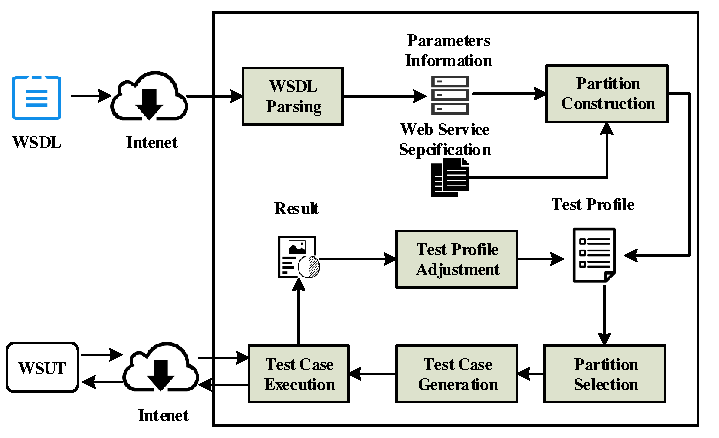
\includegraphics[width = 0.5\textwidth]{fig//framework}
  \caption{DRT for web services framework}
  \label{fig:frame}
\end{figure}

\begin{enumerate}[1]
  \item
  \emph{WSDL Parsing}.
  Web services are composed of services and the relevant WSDL documents.
  By parsing the WSDL document, we can get the input information for each operation in the services.
  This includes the number of parameters, their names and types, and any additional requirements that they may have.

  \item
  \emph{Partition Construction}.
  Partition testing (PT) refers to a class of testing techniques that break the input domain into a number of partitions~\cite{weyuker1991analyzing}.
  Because DRT is a black-box testing technique, combining RT and PT, the PT approaches used are at the specification level.
  Various approaches andprinciples for achieving convenient and effective partitions have been discussed in the literature~\cite{weyuker1991analyzing, cai2005partition, chen1994relationship, chen1996expected}.
  The input domain of the web service under test (WSUT) can be partitioned based on the WSUT specifications and the parsed parameters.
  Once partitioned, testers can assign probability distributions to the partitions as an initial testing profile.
  This initial testing profile can be assigned in different ways, including using a uniform probability distribution, or one that sets probabilities according to the importance of the partition. \textcolor{red}{For instance, a partition should be given higher priority if more faults have been detected within it in the previous testing history.}. \dpt{How is the importance determined?}

  \item
  \emph{Partition Selection}.
  DRT randomly selects a partition according to the testing profile.

  \item
  \emph{Test Case Generation}.
  Given the selected partition $s_i$, a test case is then randomly and independently generated within $s_i$.
  Because the WSDL document has been parsed, generation of this test case is non difficult, and can be automated.

  \item
  \emph{Test Case Execution}.
  The relevant DRT component receives the generated test case, converts it into an input message, invokes the web service(s) through the SOAP protocol, and intercepts the test results (from the output message).

  \item
  \emph{Test Profile Adjustment}.
  Upon completion of each test, its pass or fail status is determined by comparing the actual and expected results (with the test passing if both are the same).
  The pass or fail status is then used to adjust the (partition) probability distribution accordingly.
  Situations where determination of the test outcome status is not possible (i.e. in the presence of the oracle problem \textcolor{red}{~\cite{weyuker1982testing, barr2015oracle, patel2018mapping}}\rrf) may potentially be addressed using metamorphic testing~\cite{sun2011}.
\end{enumerate}

\dpt{I'm not sure that I have the correct intended meaning in the next paragraph. Please confirm}
Generally speaking, DRT test case generation is both in accordance with the probability distribution (for selection of the relevant partition), and with the principles of RT, taking advantage of the ease of RT and the practicability of PT. \dpt{are we sure that PT is effective?}
Furthermore, many of the DRT for web services framework components can be automated.
To make DRT for web services more efficient and practical, we developed a prototype that will be described in Section~\ref{sec:prototype}.

\subsection{Guidelines for Parameter Setting}
\label{sec:relation}

Our previous work~\cite{sun2012towards} found that the DRT performance can be influenced by the number of partitions and the parameter $\varepsilon$ \textcolor{red}{which is the adjustment of the selection probabilities of partitions.}(\dpt{shall we explain $\varepsilon$ here?}) \sout{and by the number of partitions}.
We next explore these impacts through a theoretical analysis, which, to be mathematically tractable, has the following assumptions:

\begin{enumerate}[1]
  \item
  The failure rate $\theta_i$ of each partition $s_i$ ($i = 1, 2, \ldots, m$, and $m > 1$) is unknown, but can be estimated.

  \item
  Each failure rate~$\theta_i$ ($i = 1, 2, \ldots, m$, and $m > 1$) remains unchanged throughout the testing process (faults are not removed after their detection).

  \item
  Test cases are selected with replacement, which means that same test cases may be selected more than once.
\end{enumerate}

A principle of the DRT strategy is to increase the selection probabilities (by amount $\varepsilon$) of partitions with larger failure rates.
In addition to the impact of the parameter $\varepsilon$, the number of partitions also influences the speed of updating the testing profile (Formulas \ref{eq:DRThitJ} to \ref{eq:DRTmissJ}). \dpt{why (here and elsewhere) directly using numbers here and not references/labels for the \LaTeX{} for the formulas?}
Therefore, for a given number of partitions, we are interested in investigating what values of $\varepsilon$ yield the best DRT performance.

\dpt{note that in the next paragraph I have assumed that more than one partition may have $\theta_M$}
Letting $\theta_M$ denote the maximum failure rate, and $s_M$ denote partitions with that failure rate, then $p_i^n$ denotes the probability of executing the $n^{th}$ test case from partition $s_i$.
As testing proceeds, the probability $p_M$ of partition $s_M$ being selected is expected to increase:
\begin{equation}
    \label{eq:exception}
    p_M^{n + 1} > p_M^{n}
\end{equation}

Initially, the testing profile is
$\{ \left \langle s_1,p_1^0 \right \rangle, \left \langle s_2,p_2^0 \right \rangle, \ldots, \left \langle s_m,p_m^0 \right \rangle\}$,
which, after $n$ test cases have been executed,  is then updated to
$\{ \left \langle s_1,p_1^n \right \rangle, \left \langle s_2,p_2^n \right \rangle, \ldots, \left \langle s_m,p_m^n \right \rangle\}$.
During the testing process, $p_i^n$ is increased or decreased by the value $\varepsilon$, which is relatively small (set to $0.05$ in previous studies \cite{Lv2011,li2015}).
Because the initial $p_i^0$ is larger than $\varepsilon$, and the adjustment of $p_i$ is relatively small (Formulas~\ref{eq:DRThitJ} to~\ref{eq:DRTmissJ}), the following two situations are rare, and thus not considered here:
$p_i < \varepsilon / (m - 1)$ or
$p_i < \varepsilon$ ($i = 1, 2, \ldots, m$).


As part of exploring the relationship between $p_i^{n + 1}$ and $p_i^{n}$, we calculate the conditional probability, $p(i|\delta)$, of the following four situations (denoted $\delta_1, \delta_2, \delta_3$, and $\delta_4$, respectively):

\dpt{here and elsewhere, there are full-sops after some formulas (e.g. (7). Should these be removed?}

\dpt{We'll probably need to come back later and reword/reformat some of the maths stuff}

\dpt{Please confirm that the changes I've made below are correct}

\begin{enumerate}[ {Situation} 1 ($\delta_1$):]
  \item
  \textbf{If $t_{n} \notin s_i$ and a fault is detected by $t_n$}, then $p(i|\delta_1)$ is calculated according to Formula \ref{eq:DRThitJ}:
%      \begin{equation}
%          	p(i|\delta_1) = \sum_{i \neq j}\theta_j(p_i^n - \displaystyle\frac{\varepsilon}{m - 1}).
%      \end{equation}
    $$p(i|\delta_1) = \sum_{i \neq j}\theta_j(p_i^n - \displaystyle\frac{\varepsilon}{m - 1}).$$

  \item
  \textbf{If $t_{n} \in s_i$ and a fault is detected by $t_n$}, then $p(i|\delta_2)$ is calculated according to Formula \ref{eq:DRThitI}:
%      \begin{equation}
%          p(i|\delta_2) = \theta_i(p_i^n + \varepsilon).
%      \end{equation}
    $$p(i|\delta_2) = \theta_i(p_i^n + \varepsilon).$$

  \item
  \textbf{If $t_{n} \in s_i$ and no fault is detected by $t_n$}, then $p(i|\delta_3)$ is calculated according to Formula \ref{eq:DRTmissI}:
%      \begin{equation}
%          p(i|\delta_3) = (1 - \theta_i)(p_i^n - \varepsilon).
%      \end{equation}
    $$p(i|\delta_3) = (1 - \theta_i)(p_i^n - \varepsilon).$$

  \item
  \textbf{If $t_{n} \notin s_i$ and no fault is detected by $t_n$}, then $p(i|\delta_4)$ is calculated according to Formula \ref{eq:DRTmissJ}:
%      \begin{equation}
%          p(i|\delta_4) = \sum_{i \neq j}(1 - \theta_j)(p_i^n + \displaystyle\frac{\varepsilon}{m - 1}).
%      \end{equation}
    $$p(i|\delta_4) = \sum_{i \neq j}(1 - \theta_j)(p_i^n + \displaystyle\frac{\varepsilon}{m - 1}).$$
\end{enumerate}

Therefore, $p_i^{n + 1}$ for all cases together is:

\begin{equation}
    \label{eq:7}
    \begin{split}
    p_i^{n + 1} = &p_i^n\theta_i(p_i^n + \varepsilon) + p_i^n(1-\theta_i)(p_i^n - \varepsilon)\\
    &+ \sum_{j \neq i}p_j^n\theta_j(p_i^n - \displaystyle \frac{\varepsilon}{m- 1})\\
    &+ \sum_{j \neq i}p_j^n(1 - \theta_j)(p_i^n + \displaystyle\frac{\varepsilon}{m - 1})\\
    =&(p_i^n)^2\theta_i + p_i^n\theta_i\varepsilon + (p_i^n)^2 - p_i^n\varepsilon - (p_i^n)^2\theta_i + p_i^n\theta_i\varepsilon\\
    & + (p_i^n - \displaystyle\frac{\varepsilon}{m - 1})\sum_{j \neq i}p_j^n\theta_j + (p_i^n + \displaystyle\frac{\varepsilon}{m - 1})\sum_{j \neq i}p_j^n\\
    &- (p_i^n + \displaystyle\frac{\varepsilon}{m - 1})\sum_{j \neq i}p_j^n\theta_j\\
    =&(p_i^n)^2 + 2p_i^n\theta_i\varepsilon - p_i^n\varepsilon + (p_i^n - \displaystyle\frac{\varepsilon}{m - 1} - p_i^n \\
    &- \displaystyle\frac{\varepsilon}{m - 1})\sum_{j \neq i}p_j^n\theta_j + (p_i^n + \displaystyle\frac{\varepsilon}{m - 1})(1 - p_i^n)\\
    =&p_i^n + (p_i^n)^2 - (p_i^n)^2 + 2p_i^n\theta_i\varepsilon - p_i^n\varepsilon + \displaystyle\frac{\varepsilon}{m - 1} - \\
    &\displaystyle\frac{\varepsilon}{m - 1}p_i^n - \displaystyle\frac{2\varepsilon}{m - 1}\sum_{j \neq i}p_j^n\theta_j\\
    =&p_i^n + \displaystyle\frac{\varepsilon}{m - 1}(2p_i^n\theta_im - p_i^nm - 2p_i^n\theta_i + 1 )\\
    &- \displaystyle\frac{2\varepsilon}{m-1}\sum_{j \neq i}p_j^n\theta_j\\
    =&p_i^n + Y_i^n,
    \end{split}
\end{equation}
where
\begin{equation}
    \begin{split}
    \label{eq:yi}
    Y_i^n = &\displaystyle\frac{\varepsilon}{m - 1}(2p_i^n\theta_im - p_i^nm - 2p_i^n\theta_i + 1 )\\
             &- \displaystyle\frac{2\varepsilon}{m-1}\sum_{j \neq i}p_j^n\theta_j.
    \end{split}
 \end{equation}

From Formula~\ref{eq:yi}, we have:
 \begin{equation}
    \begin{split}
    \label{eq:26}
    Y_M^n - Y_i^n = &\displaystyle\frac{\varepsilon}{m - 1}(2p_M^n\theta_Mm - p_M^nm - 2p_M^n\theta_M + 1)\\
    & - \displaystyle\frac{2\varepsilon}{m - 1}\sum_{j \neq M}p_j^n\theta_j - \displaystyle\frac{\varepsilon}{m - 1}(2p_i^n\theta_im - p_i^nm\\
    & - 2p_i^n\theta_i + 1) + \displaystyle\frac{2\varepsilon}{m - 1}\sum_{j \neq i}p_j^n\theta_j \\
    =&\displaystyle\frac{\varepsilon}{m - 1}(2m(p_M^n\theta_M - p_i^n\theta_i) - m(p_M^n - p_i^n) -\\
    & 2(p_M^n\theta_M - p_i^n\theta_i)) - \sum_{j \neq M}p_j^n\theta_j + \sum_{j \neq i}p_j^n\theta_j    \\
    =& \displaystyle\frac{2\varepsilon}{m - 1}(m(p_M^n\theta_M - p_i^n\theta_i) - \displaystyle\frac{m(p_M^n - p_i^n)}{2} - \\
    &(p_M^n\theta_M - p_i^n\theta_i)) + \displaystyle\frac{2\varepsilon}{m-1}(p_M^n\theta_M - p_i^n\theta_i)\\
    =&\displaystyle\frac{2\varepsilon}{m - 1}(m(p_M^n\theta_M - p_i^n\theta_i) - \displaystyle\frac{m(p_M^n - p_i^n)}{2}).
    \end{split}
\end{equation}

Before presenting the final guidelines, we need the following lemma.
\newtheorem{lem}{Lemma}
\label{Lemma}
\begin{lem}
  If $p_i^{n} - p_M^{n} > 2(p_i^{n}\theta_i - p_M^{n}\theta_M)$, then $p_M^{n + 1} > p_M^{n}$.
\end{lem}
\begin{IEEEproof}
%\emph{Proof:}
The condition $p_i^{n} - p_M^{n} > 2(p_i^{n}\theta_i - p_M^{n}\theta_M)$ can be equivalently expressed as:
\begin{equation}
  \label{lemma:proof1}
\displaystyle\frac{p_M^n - p_i^n}{2} < p_M^{n}\theta_M - p_i^{n}\theta_i.
\end{equation}

From Formula~\ref{lemma:proof1},  $(p_M^{n}\theta_M - p_i^{n}\theta_i) - \displaystyle\frac{p_M^n - p_i^n}{2} > 0$, and because $0 < \varepsilon < 1$, and $m > 1$,  therefore:
\begin{equation}
  \label{lemma:proof2}
\displaystyle\frac{2m\varepsilon}{m - 1}((p_M^{n}\theta_M - p_i^{n}\theta_i) - \displaystyle\frac{p_M^n - p_i^n}{2}) > 0.
\end{equation}

Furthermore:
\begin{equation}
  \label{lemma:proof3}
\displaystyle\frac{2\varepsilon}{m - 1}(m(p_M^{n}\theta_M - p_i^{n}\theta_i) - \displaystyle\frac{m(p_M^n - p_i^n)}{2}) > 0.
\end{equation}

According to Formulas \ref{lemma:proof3} and \ref{eq:26},
if $p_i^{n} - p_M^{n} > 2(p_i{n}\theta_i - p_M^{n}\theta_M)$, then
$Y_M^n - Y_i^n > 0$.

Also, because
$\sum_{i=1}^mp_i^{n + 1} = 1$, and
$\sum_{i=1}^mp_i^{n} = 1$, therefore
$Y_M^n >0$, and thus
$\sum_{i=1}^mY_i^n = 0$.

According to Formula~\ref{eq:7},
$p_M^{n + 1} = p_M^n + Y_M^n$.
Because $Y_M^n >0$, therefore
$p_M^{n + 1} > p_M^n$.
%$\hfill{}
%\Box$
\end{IEEEproof}

Accordingly, we can now present the following theorem that states a sufficient condition for achieving $p_M^{n + 1} > p_M^{n}$.
%\newtheorem{theo}{Theorem}
%\label{theorem}
%\begin{theo}
%  For all failure rates $\theta_i, i \in \{1, 2, \ldots, m\}$, and $\theta_M$ is the maximum of $\theta_i$, the following condition is sufficient to guarantee that $p_M^{n + 1} > p_M^{n}$
%\begin{equation}
%  \displaystyle\frac{1}{4\theta_M\theta_{\Delta}} < \displaystyle\frac{m + \varepsilon}{m\varepsilon} < \displaystyle\frac{1}{2\theta_\Delta}
%\end{equation}

\newtheorem{theo}{Theorem}
\label{theorem}
\begin{theo}
  For failure rate $\theta_{min} = min\{\theta_1, \ldots, \theta_m\}$, $\theta_M > \theta_{min}$, if $0 < \theta_{min} < \frac{1}{2}$, the following condition is sufficient to guarantee that $p_M^{n + 1} > p_M^{n}$:
\begin{equation}
\label{equa:results}
  \displaystyle\frac{2m\theta_{min}^2}{1-2\theta_{min}} < \varepsilon < \displaystyle\frac{(m-1)m\theta_{min}}{2(m + 1)}.
\end{equation}


%where $\theta_i \le \theta_\Delta < \theta_M$, and $\theta_i \ne \theta_M$.
\end{theo}
\emph{Proof:} In order to guarantee $p_M^{n + 1} > p_M^{n}$, we consider the following three situations (where $i \in \{1, 2, \ldots, m\}$ and $i \ne M$).

\textbf{Situation 1 ($p_i^n = p_M^n$):}
Because $\theta_i < \theta_M$, therefore
$(p_i^n\theta_i - p_M^n\theta_M) < 0$.

Therefore, $(p_i^n - p_M^n) > 2(p_i^n\theta_i - p_M^n\theta_M)$.

According to Lemma 1, we have $p_M^{n + 1} > p_M^{n}$.

%\textbf{Case 2 ($p_i^n > p_M^n$):} Since $1/2\theta_\Delta > (m + \varepsilon)/m\varepsilon$, and $1/2\theta_i \ge 1/2\theta_\Delta$, then $(p_i^n - p_M^n)\varepsilon > 2(p_i^n - p_M^n)\theta_i(m + \varepsilon)/m$, and $(p_i^n - p_M^n)\varepsilon > 2(p_i^n - p_M^n)\theta_i$. Because $\theta_M > \theta_i$, we have $2(p_i^n - p_M^n)\theta_i > 2(p_i^n\theta_i - p_M^n\theta_M)$. Then $(p_i^n - p_M^n)\varepsilon > 2(p_i^n\theta_i - p_M^n\theta_M)$. According to Lemma 1, we have $p_M^{n + 1} > p_M^{n}$.

\textbf{Situation 2 ($p_i^n > p_M^n$):} According to Formula \ref{equa:results}, we have the following:
$$\varepsilon > \displaystyle\frac{2m\theta_{min}^2}{1-2\theta_{min}}.$$

Because
$$\displaystyle\frac{2m\theta_{min}^2}{1-2\theta_{min}} = \displaystyle\frac{\theta_{min}}{1/2m\theta_{min} - 1/m},$$
we have the following:
$$\varepsilon > \displaystyle\frac{\theta_{min}}{1/2m\theta_{min} - 1/m}.$$

Because $\theta_{min} < 1/2$, therefore
$1/2m\theta_{min} - 1/m > 0$ and
$\varepsilon(1/2m\theta - 1/m) > \theta_{min}$, which gives
$\varepsilon/2m\theta_{min} > \theta_{min} + \varepsilon/m$.

Because $\varepsilon > 0$, and $m > 1$, therefore
 $$\displaystyle\frac{1}{2\theta_{min}} > \displaystyle\frac{(\theta_{min} + \varepsilon/m)}{(\varepsilon/m)}.$$

$(1/2\theta_{min})(p_i^n - p_M^n) > (p_i^n - p_M^n)(\theta_{min} + \varepsilon/m)/(\varepsilon/m)$ as
$p_i^n > p_M^n$, and
$$p_i^n -p_M^n > 2\theta_{min}(p_i^n -p_M^n)\displaystyle\frac{\theta_{min} + \varepsilon/m}{\varepsilon/m}.$$

Because $(\theta_{min} + \varepsilon/m)/(\varepsilon/m) > 1$, therefore
$$2\theta_{min}(p_i^n -p_M^n)\displaystyle\frac{\theta_{min} + \varepsilon/m}{\varepsilon/m} > 2\theta_{min}(p_i^n -p_M^n).$$

Because $\theta_{min} < \theta_M$, therefore
$$2\theta_{min}(p_i^n - p_M^n) > 2(p_i^n\theta_{min} - p_M^n\theta_M).$$

Thus,
$$p_i^n -p_M^n > 2(p_i^n\theta_{min} - p_M^n\theta_M).$$

According to Lemma 1, we have $p_M^{n + 1} > p_M^{n}$.
%Furthermore, we have $(1/2\theta_{min})(p_i^n - p_M^n) > (p_i^n - p_M^n)(\theta_{min} + \varepsilon/m)/(\varepsilon/m)$, and $p_i^n - p_M^n > 2(p_i^n - p_M^n)\theta_{min}(\theta_{min} + \varepsilon/m)/(\varepsilon/m)$. Because $2(p_i^n - p_M^n)\theta_{min}(\theta_{min} + \varepsilon/m)/(\varepsilon/m) > 2(p_i^n - p_M^n)\theta_{min}$, and $2(p_i^n - p_M^n)\theta_{min} > 2(p_i^n\theta_{min} - p_M^n)$, we have $(p_i^n - p_M^n) > 2(p_i^n\theta_i - p_M^n\theta_M)$. According to Lemma 1, $p_M^{n + 1} > p_M^{n}$ is satisfied.

%\textbf{Case 3 ($p_i^n < p_M^n$):} Since $1/2\theta_M < (m + \varepsilon)/m\varepsilon$, then $(p_M^n - p_i^n)\varepsilon < 2(p_M^n - p_i^n)\theta_M(m + \varepsilon)/m$. Because $\theta_i < \theta_M$, we have $2(p_M^n - p_i^n)\theta_M(m + \varepsilon)/m < 2(p_M^n\theta_M - p_i^n\theta_i)(m + \varepsilon)/m$. Furthermore, we have $(p_M^n - p_i^n)\varepsilon < 2(p_M^n\theta_M - p_i^n\theta_i)(m + \varepsilon)/m$, and thus $(p_i^n - p_M^n)\varepsilon > 2(p_i^n\theta_i - p_M^n\theta_M)(m + \varepsilon)/m$. According to Lemma 1, we have $p_M^{n + 1} > p_M^{n}$. $\hfill{} \Box$

\textbf{Situation 3 ($p_i^n < p_M^n$):}
For this proof, we make the assumption that $\frac{1}{2} < \theta_M < 1$.

Because we have
$$\varepsilon < \displaystyle\frac{(m - 1)m\theta_{min}}{2(m + 1)}$$
and
$$\displaystyle\frac{(m - 1)m\theta_{min}}{2(m + 1)} = \displaystyle\frac{2m -(m + 1)}{2(m + 1)}m\theta_{min},$$
thus
$$\varepsilon < (\displaystyle\frac{m}{m +1} - \displaystyle\frac{1}{2})m\theta_{min}.$$

Obviously, $\varepsilon/m < (m/(m + 1) - 1/2)\theta_{min}$ as $m > 1$.

Furthermore, we have
$$-\displaystyle\frac{\varepsilon}{m} > (\displaystyle\frac{1}{2} - \displaystyle\frac{m}{m + 1})\theta_{min}$$
and
$$\displaystyle\frac{m\theta_{min}}{m + 1} - \displaystyle\frac{\varepsilon}{m} + \displaystyle\frac{2\varepsilon}{m} > \displaystyle\frac{\theta_{min}}{2} + \displaystyle\frac{2\varepsilon}{m}$$
which means that
$$\displaystyle\frac{m\theta_{min}}{m + 1} + \displaystyle\frac{\varepsilon}{m}  > \displaystyle\frac{1}{2}(\theta_{min} + \displaystyle\frac{4\varepsilon}{m}).$$

It follows that
$$(m\theta_{min}/(m + 1) + \varepsilon/m)/(4\varepsilon/m + \theta_{min}) > 1/2$$ for any $m > 1, \varepsilon > 0$, and $0 < \theta_{min} < 1$.

Because $\frac{1}{2} < \theta_M < 1$, therefore
$(m\theta_{min}/(m + 1) + \varepsilon/m)/(4\varepsilon/m + \theta_{min}) > 1/2\theta_M$.

Thus, we have
$$2(p_M^n -p_i^n)\theta_M\displaystyle\frac{\displaystyle\frac{\varepsilon}{m} +\displaystyle\frac{m\theta_{min}}{m + 1}}{\displaystyle\frac{4\varepsilon}{m} + \theta_{min}} > p_M^n -p_i^n$$
as $p_M^n > p_i^n$.

Because $\varepsilon/m < 4\varepsilon/m$, and $m\theta_{min}/(m + 1) < \theta_{min}$, therefore
$$ \displaystyle\frac{\displaystyle\frac{\varepsilon}{m} +\displaystyle\frac{m\theta_{min}}{m + 1}}{\displaystyle\frac{4\varepsilon}{m} + \theta_{min}} < 1$$
and
$$ 2(p_M^n -p_i^n)\theta_M > 2(p_M^n -p_i^n)\theta_M\displaystyle\frac{\displaystyle\frac{\varepsilon}{m} +\displaystyle\frac{m\theta_{min}}{m + 1}}{\displaystyle\frac{4\varepsilon}{m} + \theta_{min}}$$

Hence we have
$$2(p_M^n -p_i^n)\theta_M > p_M^n -p_i^n,$$
which can be equivalently expressed as
$$p_i^n -p_M^n > 2(p_i^n - p_M^n)\theta_M.$$

Because $\theta_{min} < \theta_M$, therefore
$2(p_i^n - p_M^n)\theta_M > 2(p_i^n\theta_{min} - p_M^n\theta_M)$, and thus
$$p_i^n -p_M^n > 2(p_i^n\theta_{min} - p_M^n\theta_M).$$

According to Lemma 1, we have $p_M^{n + 1} > p_M^{n}$.
$\hfill{}
\Box$

%Since $\varepsilon < (m - 1)m\theta_{min}/2(m + 1)$, and $\varepsilon < (m/(m + 1) - 1/2)m\theta_{min}$, then, $\varepsilon/m < (m/(m + 1) - 1/2)\theta_{min}$, and $-\varepsilon/m > (1/2 - m/(m +1))\theta_{min}$. Furthermore, we have $\varepsilon/m + m\theta_{min}/(m + 1) > 2\varepsilon/m + \theta_{min}/2$, and thus $((\varepsilon/m + m\theta_{min})/(m + 1))/(4\varepsilon/m + \theta_{min}) > 1/2\theta_M$. Because $p_M^n > p_i^n$, we have $2(p_M^n -p_i^n)\theta_M((\varepsilon/m + m\theta_{min}/(m + 1))/(4\varepsilon/m + \theta_{min})) > (p_M^n - p_i^n)$. Since $\varepsilon/m < 4\varepsilon/m$, and $m\theta_{min}/(m + 1) < \theta_{min}$, we have $((\varepsilon/m + m\theta_{min}/(m + 1))/(4\varepsilon/m + \theta_{min})) < 1$, and $2(p_M^n - p_i^n)\theta_M > p_M^n - p_i^n$. Because $2(p_M^n\theta_M - p_i^n\theta_{min}) > 2(p_M^n - p_i^n)\theta_M$, we have $2(p_M^n\theta_M - p_i^n\theta_{min}) > p_M^n - p_i^n$, and $p_i^n - p_M^n > 2(p_i^n\theta_{i} - p_M^n\theta_M)$. According to Lemma 1, $p_M^{n + 1} > p_M^{n}$ is satisfied. $\hfill{} \Box$

In summary, when $\frac{1}{2} < \theta_M < 1$, there is always an interval $E$:
\dpt{Is ``$E$'' the correct notation?}
\begin{equation}
  \varepsilon \in (\displaystyle\frac{2m\theta_{min}^2}{1 - 2\theta_{min}}, \displaystyle\frac{(m - 1)m\theta_{min}}{2(m + 1)})
\end{equation}
where $\theta_{min} \le \theta_i, i \in \{1, 2, \ldots, m\}$, and $\theta_i \ne 0$, which can guarantee $p_M^{n+1} > p_M^n$.

From the proof above, it is clear that the value of $\theta_M$ affects the upper bound ($E_{upper}$) of $E$.
When $\theta_{min} < \theta_M < \frac{1}{2}$, the value of $E_{upper}$ should close to the lower bound of $E$.
In practice, we should set
\begin{equation}
\label{euqtion:approxValue}
  \varepsilon \approx \frac{2m\theta_{min}^2}{1-2\theta_{min}}.
\end{equation}

\subsection{Prototype}
\label{sec:prototype}

Figure~\ref{fig:prototype} shows a screenshot of a prototype tool that partially automates DRT for web services.
To start, testers input the address of the web service being tested (the URL of the WSDL), and press the Parse button to analyze the input and output formats.
Next, an operation is selected from the operation list (in the bottom left).
The tool provides two options for the partitions and test suites:
\dpt{I assume that automatically generating the partitions will also mean automatically generating the test cases. Please confirm.}
either to automatically generate the partitions (and test cases); or
to upload the predefined partitions and test suites.
Before beginning testing (by pressing the Test button), testers must set the maximum number of tests (Test Repetition Limit).
During the testing, if a failure is detected before having executed the maximum number of tests, then the tool suspends testing and asks for the tester's instruction.
Testers can choose to remove defects and continue testing, or to stop testing.
When all tests have completed, the test report is summarized and output in a file.

\begin{figure}[!htp]
  \centering
  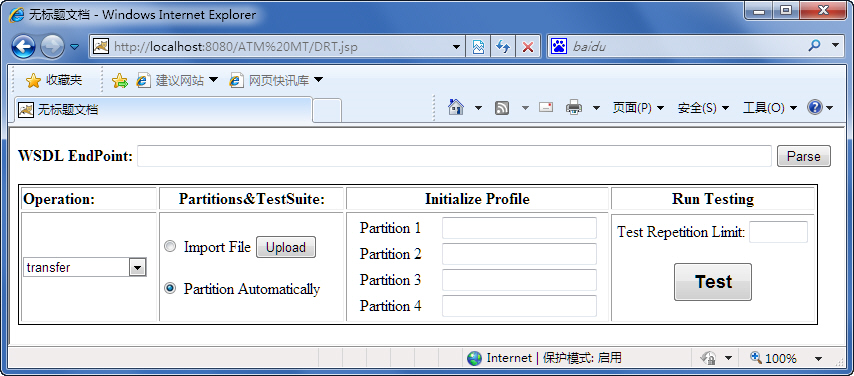
\includegraphics[width=0.5\textwidth]{fig//prototype}
  \caption{Prototype interface}
  \label{fig:prototype}
\end{figure}

\section{Empirical Study}
\label{sec:empiricalstudy}

We conducted a series of empirical studies to evaluate the performance of DRT.

\subsection{Research Questions}

In our experiments, we focused on addressing the following three research questions:

\begin{description}
  \item [RQ1] How effective is DRT at detecting web service faults?

  Fault-detection effectiveness is a key criterion for evaluating the performance of a testing technique.
  In our study, we chose three commonly used, real-life web services as subject programs, and applied mutation analysis to evaluate the effectiveness.

  \item [RQ2] How do the number of partitions and the DRT parameter $\varepsilon$ impact on the failure detection efficiency \textcolor{red}{and effectiveness} of DRT?
  \dpt{efficiency or effectiveness?}

  In our earlier work~\cite{sun2012towards}, we found that the DRT parameter $\varepsilon$ had a significant effect on DRT efficiency, and  that the optimal value of the parameter could be related to the number of partitions.
  The relationship between $\varepsilon$ and the number of partitions is examined through theoretical analysis, and verified through the empirical studies.

  \item [RQ3] What is the actual test case generation overhead when using the DRT strategy?

  In Section~\ref{sec:DRTStrategy}, we have showed that DRT only requires linear time to generate test case.
  We wish to validate this theoretical finding through empirical examination of the actual test case generation and execution.
\end{description}

\subsection{Subject Web Services}

We selected three real-life web services as the subject programs for our study:
\texttt{Aviation Consignment Management Service (ACMS)},
\texttt{China Unicom billing service (CUBS)}, and
\texttt{Parking billing service (PBS)}.
We used mutation analysis to generate a total of 1563 mutants.
After removing equivalent mutants, we then also removed mutants that were too easily detected
---
deleting mutants that could be detected with less than 20 randomly generated test cases.
Table~\ref{tab:objects} summarizes the basic information of the used web services and their mutants.
A detailed description of each web service is given in the following.

%In our study, we selected three real-life web services, namely \texttt{Aviation Consignment Management Service\\ (ACMS)}, \texttt{China Unicom billing service (CUBS\\)}, \texttt{Parking billing service (PBS)}, as the subject programs of the experiments.
%Mutation analysis help us generate 1563 mutants for all objects. After identifying equivalent mutants, we only include those mutants being hard to detect for the evaluation.
%Further to say, every those mutants cannot be detected with less than 20 randomly generated test cases.
%Table~\ref{tab:objects} summarizes the basic information of the object web services.
%In following section, we give a detailed description of each web services.

\begin{table}[!htp]
\caption{Studied Web Services}
\label{tab:objects}
\centering
\begin{tabular}{|c|c|c|} \hline
  Web service           &LOC           &Number of mutants \\ \hline
  ACMS    &116           &3   \\ \hline
  CUBS       &131           &11   \\ \hline
  PBS            &129           &4    \\ \hline
\end{tabular}

\end{table}

\subsubsection{Aviation Consignment Management Service (ACMC)}

ACMS helps airline companies check the allowance (weight) of free baggage, and the cost of additional baggage.
Based on the destination, flights are categorised as either domestic or international.
For international flights, the baggage allowance is greater if the passenger is a student (30kg), otherwise it is 20kg.
Each aircraft offers three cabins classes from which to choose (economy, business, and first), with passengers in different classes having different allowances.
The detailed price rules are summarized in Table~\ref{tab:aviation}, where $price_0$ means economy class fare.

\begin{table*}[!htp]
  \caption{ACMC Baggage Allowance and Pricing Rules}
  \label{tab:aviation}
  \centering
  \begin{tabular}{|c|c|c|c|c|c|c|} \hline
  \multirow{2}{*}{}     &\multicolumn{3}{c|}{Domestic flights}              &\multicolumn{3}{c|}{International flights} \\
  \cline{2-7}
                       &First class  &Business class   &Economy class   &First class  &Business class   &Economy class \\ \hline
  Carry~on (kg)   &5       &5        &5        &7        &7        &7  \\ \hline
  Free checked-in (kg)   &40      &30       &20       &40       &30       &20/30 \\ \hline
  Additional baggage pricing~(kg)   &\multicolumn{3}{c|}{$price_0 * 1.5\%$}   &\multicolumn{3}{c|}{$price_0 * 1.5\%$}  \\ \hline
  \end{tabular}
\end{table*}

\subsubsection{China Unicom Billing Service (CUBS)}

CUBS provides an interface through which customers can know how much they need to pay according to cell-phone plans, calls, and data usage.
The details of several cell-phone plans are summarized in Tables~\ref{table:chinaA},~\ref{table:chinaB}, and~\ref{table:chinaC}.
\dpt{Please check the tables: it seems strange to talk about Plan A/B/C as the heading of each table, and then have column headings in each table for $plan_1$, etc.}
\dpt{There also seem to be some formatting issues for the tables --- width, etc. It may be a good idea to also check what kind of formatting style the journal wants (all capitals; title case, etc.)}

% cell-phone plan~(CNY)
%\begin{table*}[!htp]
%  \caption{Cell-phone plan A}
%  \label{table:chinaA}
%  \centering
%  \begin{tabular}{|c|c|c|c|c|c|c|c|c|c|c|c|c|} \hline
%  \multicolumn{2}{|c|}{\mulitirow{2}{*}{}}                 &46  &66  &96  &126  &156  &186  &226  &286  &386  &586  &886 \\ \hline
%  \rule{0pt}{8pt}\multirow{3}{*}{\rotatebox{90}{contains}} &free calls~(min)  &50  &50  &240  &320  &420  &510  &700 &900 &1250 &1950  &3000 \\ \cline{2-13}
%  \rule{0pt}{8pt}                                          &free data~(MB)  &150 &300 &300  &400  &500  &650  &750 &950 &1300 &2000  &3000 \\ \cline{2-13}
%  \rule{0pt}{8pt}                                          &free incoming calls  &\multicolumn{11}{c|}{domestic~(including video calls)} \\ \hline
%  \rule{0pt}{8pt}\multirow{3}{*}{\rotatebox{90}{overuse}} &incoming calls~(CNY/min)  &0.25 &0.20  &\multicolumn{9}{c|}{0.15} \\ \cline{2-13}
%  \rule{0pt}{8pt}                                          &data~(CNY/KB)  &\multicolumn{11}{c|}{0.0003} \\ \cline{2-13}
%  \rule{0pt}{8pt}                                          &video calls~(CNY/min)  &\multicolumn{11}{c|}{0.60} \\ \hline
%  \end{tabular}
%\end{table*}


\begin{table*}[!htp]
  \caption{Plan A}
  \label{table:chinaA}
  \centering
  \resizebox{\textwidth}{12mm}{
  \begin{tabular}{|c|c|c|c|c|c|c|c|c|c|c|c|c|} \hline
  \multicolumn{2}{|c|}{\multirow{2}{*}{Plan details}}                 &\multicolumn{11}{|c|}{Month charge~(CNY)} \\ \cline{3-13}
  \multicolumn{2}{|c|}{}                                                        &\!$option_1$\!  &\!$option_2$\!  &\!$option_3$\!  &\!$option_4$\!  &\!$option_5$\!  &\!$option_6$\! &\!$option_7$\!  &\!$option_8$\!  &\!$option_9$\!  &\!$option_{10}$\!  &\!$option_{11}$\! \\ \hline
  \multirow{3}{*}{\rotatebox{90}{Basic}} &Free calls~(min)  &50  &50  &240  &320  &420  &510  &700 &900 &1250 &1950  &3000 \\ \cline{2-13}
                                            &Free data~(MB)  &150 &300 &300  &400  &500  &650  &750 &950 &1300 &2000  &3000 \\ \cline{2-13}
                                            &Free incoming calls  &\multicolumn{11}{c|}{Domestic~(including video calls)} \\ \hline
  \multirow{3}{*}{\rotatebox{90}{Extra}} &Incoming calls~(CNY/min)  &0.25 &0.20  &\multicolumn{9}{c|}{0.15} \\ \cline{2-13}
                                           &Data~(CNY/KB)  &\multicolumn{11}{c|}{0.0003} \\ \cline{2-13}
                                            &Video calls~(CNY/min)  &\multicolumn{11}{c|}{0.60} \\ \hline
  \end{tabular}}
\end{table*}

%\begin{table}[!htp]
%  \caption{Plan B}
%  \label{table:chinaB}
%  \centering
%\setlength{\tabcolsep}{1mm}{
%  \begin{tabular}{|c|c|c|c|c|c|c|c|} \hline
%    \multicolumn{2}{|c|}{\multirow{2}{*}{Plan details}}   &\multicolumn{6}{|c|}{cell-phone plan} \\ \cline{3-8}
%    \multicolumn{2}{|c|}{}                                  &$plan_1$  &$plan_2$  &$plan_3$  &$plan_4$  &$plan_5$  &$plan_6$   \\ \hline
%    \rule{0pt}{8pt}\multirow{3}{*}{\rotatebox{90}{Basic}} &free calls~(min)  &120  &200  &450  &680  &920  &1180 \\ \cline{2-8}
%    \rule{0pt}{8pt}                                          &free data~(MB)  &40 &60 &80  &100  &120  &150 \\ \cline{2-8}
%    \rule{0pt}{8pt}                                          &free incoming calls  &\multicolumn{6}{c|}{domestic~(including video calls)} \\ \hline
%    \rule{0pt}{8pt}\multirow{3}{*}{\rotatebox{90}{Extra}} &incoming calls~(CNY/min)  &0.25 &0.20  &\multicolumn{4}{c|}{0.15} \\ \cline{2-8}
%    \rule{0pt}{8pt}                                          &data~(CNY/KB)  &\multicolumn{6}{c|}{0.0003} \\ \cline{2-8}
%    \rule{0pt}{8pt}                                          &video calls~(CNY/min)  &\multicolumn{6}{c|}{0.60} \\ \hline
%  \end{tabular}}
%\end{table}

\begin{table*}[!htp]
  \caption{Plan B}
  \label{table:chinaB}
  \centering
\setlength{\tabcolsep}{1mm}{
  \begin{tabular}{|c|c|c|c|c|c|c|c|} \hline
    \multicolumn{2}{|c|}{\multirow{2}{*}{Plan details}}   &\multicolumn{6}{|c|}{Month charge~(CNY)} \\ \cline{3-8}
    \multicolumn{2}{|c|}{}                                  &\!$option_1$\!  &\!$option_2$\!  &\!$option_3$\!  &\!$option_4$\!  &\!$option_5$\!  \!&$option_6$\!   \\ \hline
    \multirow{3}{*}{\rotatebox{90}{Basic}} &Free calls~(min)  &120  &200  &450  &680  &920  &1180 \\ \cline{2-8}
                                              &Free data~(MB)  &40 &60 &80  &100  &120  &150 \\ \cline{2-8}
                                              &Free incoming calls  &\multicolumn{6}{c|}{Domestic~(including video calls)} \\ \hline
    \multirow{3}{*}{\rotatebox{90}{Extra}} &Incoming calls~(CNY/min)  &0.25 &0.20  &\multicolumn{4}{c|}{0.15} \\ \cline{2-8}
                                              &Data~(CNY/KB)  &\multicolumn{6}{c|}{0.0003} \\ \cline{2-8}
                                              &Video calls~(CNY/min)  &\multicolumn{6}{c|}{0.60} \\ \hline
  \end{tabular}}
\end{table*}



\begin{table}[!htp]
  \caption{Plan C}
  \label{table:chinaC}
  \centering
  \begin{tabular}{|c|c|c|c|c|} \hline
  \multicolumn{2}{|c|}{\multirow{2}{*}{Plan details}}  &\multicolumn{3}{|c|}{Month charge~(CNY)} \\ \cline{3-5}
  \multicolumn{2}{|c|}{}                                  &$option_1$  &$option_2$  &$option_3$ \\ \hline
   \multirow{3}{*}{\rotatebox{90}{Basic}} &Free calls~(min)  &260  &380  &550 \\ \cline{2-5}
                                          &Free data~(MB)  &40 &60 &80 \\ \cline{2-5}
                                            &Free data~(MB)  &\multicolumn{3}{c|}{Domestic~(including video calls)} \\ \hline
   \multirow{3}{*}{\rotatebox{90}{Extra}} &Incoming calls~(CNY/min)  &0.25 &0.20  &0.15 \\ \cline{2-5}
                                            &Data~(CNY/KB)  &\multicolumn{3}{c|}{0.0003} \\ \cline{2-5}
                                            &Video calls~(CNY/min)  &\multicolumn{3}{c|}{0.60} \\ \hline
  \end{tabular}
\end{table}


%\begin{table}[!htp]
%  \caption{Cell-phone plan C}
%  \label{table:chinaC}
%  \centering
%  \begin{tabular}{|c|c|c|c|c|} \hline
%  \multicolumn{2}{|c|}{cell-phone plan~(CNY)}  &46  &66  &96   \\ \hline
%  \rule{0pt}{8pt} \multirow{3}{*}{\rotatebox{90}{contains}} &free calls~(min)  &260  &380  &550 \\ \cline{2-5}
%  \rule{0pt}{8pt}                                          &free data~(MB)  &40 &60 &80 \\ \cline{2-5}
%  \rule{0pt}{8pt}                                          &free data~(MB)  &\multicolumn{3}{c|}{domestic~(including video calls)} \\ \hline
%  \rule{0pt}{8pt} \multirow{3}{*}{\rotatebox{90}{overuse}} &incoming calls~(CNY/min)  &0.25 &0.20  &0.15 \\ \cline{2-5}
%  \rule{0pt}{8pt}                                          &data~(CNY/KB)  &\multicolumn{3}{c|}{0.0003} \\ \cline{2-5}
%   \rule{0pt}{8pt}                                         &video calls~(CNY/min)  &\multicolumn{3}{c|}{0.60} \\ \hline
%  \end{tabular}
%\end{table}

\subsubsection{Parking Billing Service (PBS)}

Consider a parking billing service that accepts the parking details for a vehicle, including the vehicle type, day of the week, discount coupon, and hours of parking.
This service  rounds up the parking duration to the next full hour, and then calculates the parking fee for according to the hourly rates in Table~\ref{tab:hourlyRate}.
If a discount voucher is presented, a 50\% discount off the parking fee is applied.
\dpt{Should the \$ signs be on the left side, not right, of the figures in Table~\ref{tab:hourlyRate}.}

\begin{table*} [!htp]\small
  \caption{Hourly Parking Rates}
  \label{tab:hourlyRate}
  \centering
  \begin{tabular}{|c|c|c|c|c|c|c|} \hline
  \multirow{3}{*}{Actual parking hours}                        &\multicolumn{6}{|c|}{Hourly parking rates} \\ \cline{2-7}
                                   &\multicolumn{3}{|c|}{Weekday}     &\multicolumn{3}{|c|}{Saturday and sunday} \\ \cline{2-7}
                                  &Motorcycle  &Car: 2-door coupe  &Car: others    &Motorcycle  &Car: 2-door coupe  &Car: others \\ \hline
  $(0.0,2.0]$                     &\$4.00        &\$4.50          &\$5.00      &\$5.00        &\$6.00        &\$7.00 \\ \hline
  $(2.0,4.0]$                     &\$5.00        &\$5.50          &\$6.00      &\$6.50      &\$7.50        &\$8.50  \\ \hline
  $(4.0,24.0]$                    &\$6.00        &\$6.50          &\$7.00      &\$8.00      &\$9.00        &\$10.00  \\ \hline
  \end{tabular}
\end{table*}

To facilitate better parking management, at the time of parking, customers may provide an estimation of parking duration, in terms of three different time ranges ($(0.0,2.0]$, $(2.0,4.0]$, and $(4.0,24.0]$).
If the estimation and actual parked hours fall into the same time range, then the customer will receive a 40\% discount;
but if they are different ranges, then a 20\% markup is applied.
A customer may choose to either use a discount coupon, or provide an estimation of parking duration, but may not do both.
(Obviously, a customer may also choose to neither provide an estimation, nor use a discount coupon.)
No vehicles are allowed to remain parked for two consecutive days on a continuous basis.

\subsection{Variables}

\subsubsection{Independent Variables}

The independent variable in this study is the testing technique, DRT.
RPT and RT were used as baseline techniques for comparison.

\subsubsection{Dependent Variables}

The dependent variable for RQ1 is the metric for evaluating the fault-detection effectiveness.
Several effectiveness metrics exist, including:
the P-measure\textcolor{red}{\cite{duran1984evaluation}} (the probability of at least one fault being detected by a test suite);
the E-measure\textcolor{red}{\cite{chen1997optimal}} (the expected number of faults detected by a test suite);
the F-measure\textcolor{red}{\cite{sun2018adaptive}} (the expected number of test cases executions required to detect the first fault); and
the T-measure\textcolor{red}{\cite{zhang2014history}} (the expected number of test cases required to detect all faults).
\dpt{Perhaps some references for the different measures?}
\textcolor{red}{In some related work such as \cite{Cai07, cai2009random, Lv2011, Yang2014Dynamic, li2015, zhang2014history},
the F-measure and T-measure are used for evaluating the fault-detection efficiency and effectiveness of the DRT testing technique. Therefore, we also employ the F-measure and T-measure as metrics to evaluate the fault-detection efficiency and effectiveness of different techniques.} \dpt{why?}
We use $F$ and $T$ to represent the F-measure and the T-measure of a testing method. %, and $SD_{measure}$ to represent the standard deviation.
As shown in Algorithm~\ref{alg:DRT}, the testing process may not terminate after the detection of the first fault.
Furthermore, because the fault detection information can lead to different probability profile adjustment mechanisms, it is also important to see what would happen after the first fault is revealed.
For our study, therefore, we introduce the F2-measure\textcolor{red}{\cite{sun2018adaptive}}, which is the number of additional test cases required to reveal the second fault after detection of the first fault.
We use $F2$ to represent the F2-measure of a testing method, and $SD_{measure}$ to represent the standard deviation of metrics (where $measure$ can be $F$, $F2$, or $T$).

An obvious metric for RQ3 is the time required to detect faults.
Corresponding to the T-measure, in this study we used $T$-$time$, the time required to detect all faults.
$F$-$time$ and $F2$-$time$ denote the time required to detect the first fault, and the additional time needed to detect the second fault (after detecting the first), respectively.

For each of these metrics, smaller values indicate a better performance.

\subsection{Experimental Settings}

\subsubsection{Partitioning}
\dpt{do we need to explain contracts?}
\textcolor{red}{In our study, we set the partitions by making use of the decision table (DT) \cite{gettys1986if} that is a schema-specific learning algorithm modeling. DT can present a large amount of complex information in a simple, straightforward manner, and is defined as a table representing a set of decision rules under all exclusive conditional scenarios in a pre-defined problem. Usually, a DT consists of four parts. The upper left part of a DT is a list of all the conditions denoted as $C_i$ for $i = 1, \ldots, c$, where c is the number of conditions in the pro-defined problem and $c \ge 1$. A set $CS_i = \{S_{i1}, \ldots, S_{it_{i}}\}$ contains all the possible states that $C_i$ can attain, where $t_i$ is the number of alternative states for $i$th condition $C_i$. In a DT the upper right part is a its condition space that is a Cartesian product of all the $CS_i$, as shown below:}
\textcolor{red}{$$ SP(C) = CS_1 \times CS_2 \times \ldots \times CS_c.$$}
\textcolor{red}{Each element in the $SP(C)$ is a condition entry (CE) with ordered $c$-tuple.}

\textcolor{red}{All possible actions make up of the lower left part of a DT, which represent as $A_j$ for $j = 1, \ldots, m$, where $m$ is the number of possible actions and $m \ge 1$. Similar to $CS_i$, an action-state set $AS_j = \{S_{j1}, \ldots, S_{jk_j}\}$ contains all the obtainable states for action $A_j$, where $k_j$ is the number of alternatives for $A_j$. The lower right part of a DT is its action space $SP(A)$, which is also a Cartesian product of the all the action sets $AS_j (j = 1, \ldots, m$, as shown below:}
\textcolor{red}{$$ SP(A) = AS_1 \times AS_2 \times \ldots \times AS_m.$$}
\textcolor{red}{Similar to $CE$, each element in the $SP(A)$ is an action entry (AE) with ordered $m$-tuple.}

%According to the above description, a complete DT is a matrix, and each column is called a \emph{rule}.
%
%In our study, we made use of a decision table~\cite{gettys1986if, tao2017entropy} to set the partitions.
%A decision table is based on a simple principle of sets of actions for sets of constraints, and can be used to present a large amount of complex information in a simple, straightforward manner.
%Constraints are the pre-conditions of a contract, and need to be resolvable to true or false. \dpt{do we need to explain contracts?}
%Actions specify valid system responses with respect to constraints, and are called \emph{rules}.
%They represent the post-conditions of a contract.
%Thus, every rule of the decision table defines a \emph{contract}.
%\sout{In our study, every \emph{contract} corresponds to a partition.}

\textcolor{red}{After constructing a DT, we can obtain a coarse one by grouping those $CE$ with the same $AE$ as a \emph{rule}, and original DT can be be considered as fine in terms of granularity. Every \emph{rule} in a DT corresponds to a partition. Therefore, according to fine and coarse DT, we can obtain two partition schemes shown in Table~\ref{tab:partition}.}

%After constructing a DT
%To investigate the performance of the three testing techniques under different scenarios, we took advantage of DT to develop the two partition schemes shown in Table~\ref{tab:partition}:
%\begin{itemize}
%\item \textbf{Scheme 1}: \textcolor{red}{Every \emph{rule} in a DT corresponds to a partition.}
%\item \textbf{Scheme 2}: \textcolor{red}{After constructing a DT, we group those $CE$ with the same $AE$ as a \emph{rule} , then every \emph{rule} in the DT corresponds to a partition.}
%\end{itemize}
\dpt{this repeats the last line of the previous paragraph ...}
\dpt{I'm not sure that I understand the intended meaning here. Can you explain or rephrase?}
\dpt{scheme or schema? Please decide. Do note that some figures have ``schema'' written in them}

\begin{table}[!htbp]
\caption{Two Partition Schemes}
\label{tab:partition}
\centering
\begin{tabular}{|c|c|c|} \hline
  Web service      &Scheme 1         &Scheme 2  \\ \hline
  ACMS  &24                &7          \\ \hline
  CUBS      &20                &3          \\ \hline
  PBS      &18                &3          \\ \hline
\end{tabular}
\end{table}

\subsubsection{Initial Test Profile}

\dpt{Please check that I have the correct meaning in the following}
Because test cases may be generated randomly during the test process, a feasible method is to use a uniform probability distribution as the initial testing profile.
On the other hand, testers may also use past experience to guide a different probability distribution as the initial profile.

\subsubsection{Constants}

In the experiments,  we were interested in exploring the relationship between the number of partitions and the DRT strategy parameter $\varepsilon$, and therefore selected a set of parameter values:
$\varepsilon \in \{1.0E$-$05, 5.0E$-$05, 1.0E$-$04, 5.0E$-$04, 1.0E$-$03, 5.0E$-$03, 1.0E$-$02, 5.0E$-$02, 1.0E$-$01, 2E$-$01, 3E$-$01, 4E$-$01, 5E$-$01\}$.
It should be noted that $\varepsilon = 5E$-$01$ is already a large value.
Consider the following scenario.
For PBS, when the test is carried out under partition scheme 2, if $\varepsilon = 7.5E$-$01$ and  a uniform probability distribution is used as the testing profile (that is, $p_i = 1/3$) , then suppose that the first test case belonging to $c_1$ is executed and does not reveal any faults, then, according to Formula 3, the value of $p_1$ would become $0$.
It is important, therefore, that the initial value of $\varepsilon$ should not be set too large.

\subsection{Experimental Environment}

Our experiments were conducted on a virtual machine running the Ubuntu 11.06 64-bit operating system, with two CPUs, and a memory of 2GB.
The test scripts were written in Java.
To ensure statistically reliable values of the metrics (F-measure, F2-measure, T-measure, F-time, F2-time, T-time), each testing session was repeated 30 times \textcolor{red}{which is following the guidelines of \cite{arcuri2011practical}} with 30 different seeds, and the average value calculated.
\dpt{Is 30 enough times? Do we have evidence? Why ``30''?}

\subsection{Threats To Validity}

\subsubsection{Internal Validity}

A threat to internal validity is related to the implementations of the testing techniques, which involved a moderate amount of programming work.
However, our code was cross-checked by different individuals, and we are confident that all techniques were correctly implemented.

\subsubsection{External Validity}

\dpt{the threats to external validity seem quite strong. Have we any other arguments to defend against this/these threat(s)?}
\textcolor{red}{The possible threat to external validity is concerned with object programs and the faults under study. We considered three web services in our study, while there objects are real-life and frequently-used web services.}
\sout{An obvious possible threat to external validity is that we only considered three web services in the study.
However, these are real-life services.}
Furthermore, \sout{17}\textcolor{red}{18} distinct faults \textcolor{red}{which could be detected with more than 20 randomly generated test cases, were used to evaluate the performance.} \dpt{Can we elaborate on ``17 distinct faults''?} Although we have tried to improve the generalisability of the findings by applying different partitioning granularities, and 13 kinds of parameters, we cannot be certain as to whether or not similar results would be observed in other types of web services.

\subsubsection{Construct Validity}

The metrics used in our study are simple in concept and straightforward to apply, and hence there should be little threat to the construct validity.

\subsubsection{Conclusion Validity}

We have run a sufficient number of trials to ensure the statistical reliability of our experimental results. \dpt{Are we sure? How do we know?}
Furthermore, as will be discussed in Section~\ref{sec:results}, statistical tests were conducted to confirm the significance of our results.

\begin{table*}
  \caption{ACMS Results}
  \label{result:aviation}
  \centering
  \begin{tabular}{|c|c|c|c|c|c|c|c|c|c|c|c|c|c|} \hline
     \multicolumn{2}{|c|}{\multirow{2}{*}{Strategy}} &\multicolumn{6}{|c|}{Partition scheme 1} &\multicolumn{6}{|c|}{Partition scheme 2}\\ \cline{3-14}
     \multicolumn{2}{|c|}{}  &F       &$SD_F$  &F2    &$SD_{F2}$  &T     &$SD_T$  &F     &$SD_F$  &F2    &$SD_{F2}$  &T     &$SD_T$  \\ \hline
     \multicolumn{2}{|c|}{RT}  &13.30   &10.34   &14.90 &24.64      &41.80 &27.13   &13.30 &10.34   &14.90 &24.64      &41.80 &27.13   \\ \hline
     \multicolumn{2}{|c|}{RPT} &12.04   &11.13   &12.26 &19.08      &35.31 &25.95   &9.03  &8.24    &15.13 &16.08      &34.29 &29.53   \\ \hline
     \multirow{13}{*}{DRT} &1.0E-5  &11.42  &10.16  &11.93  &18.62  &34.93  &22.46  &8.73   &9.88   &13.28  &18.83  &36.19  &28.96  \\ \cline{2-14}
                           &5.0E-5	&12.42	&10.63	&12.05	&20.27	&36.90	&25.39	&8.65	&9.30	&13.53	&19.07	&35.76	&29.86 \\ \cline{2-14}
                           &1.0E-4	&11.34	&10.65	&11.66	&21.27	&35.19	&26.01	&7.36	&8.49	&13.09	&17.89	&33.00	&27.94 \\ \cline{2-14}
                           &5.0E-4	&12.16	&12.13	&11.50	&19.36	&34.19	&26.18	&7.80	&8.37	&13.45	&17.36	&33.59	&27.67 \\ \cline{2-14}
                           &1.0E-3	&11.46	&11.10	&11.39	&19.01	&34.86	&23.17	&7.68	&8.11	&15.07	&19.85	&33.65	&29.95 \\ \cline{2-14}
                           &5.0E-3	&11.02	&9.67	&12.24	&18.83	&32.92	&20.75	&7.47	&8.65	&15.40	&18.81	&35.14	&29.01 \\ \cline{2-14}
                           &1.0E-2	&10.48	&9.60	&9.46	&14.17	&29.59	&19.10	&7.66	&9.18	&14.93	&18.69	&34.30	&30.15 \\ \cline{2-14}
                           &5.0E-2	&8.75	&6.59	&7.06	&10.35	&23.05	&11.67	&7.26	&7.74	&14.70	&18.15	&34.81	&28.14 \\ \cline{2-14}
                           &1.0E-1	&8.59	&6.66	&6.37	&9.41	&21.36	&10.81	&6.67	&7.34	&16.26	&17.54	&34.27	&27.48 \\ \cline{2-14}
                           &2.0E-1	&8.50	&6.21	&5.80	&9.07	&22.10	&10.56	&5.71	&6.04	&16.63	&10.33	&33.58	&30.78 \\ \cline{2-14}
                           &3.0E-1	&9.23	&6.84	&7.12	&10.34	&22.57	&11.13	&5.43	&6.28	&17.60	&10.39	&33.86	&30.33 \\ \cline{2-14}
                           &4.0E-1	&9.22	&7.03	&6.72	&9.36	&22.57	&10.44	&5.14	&5.19	&17.56	&19.11	&33.83	&28.94 \\ \cline{2-14}
                           &5.0E-1	&8.61	&6.41	&7.70	&10.45	&22.64	&10.95	&5.86	&6.50	&16.18	&17.06	&33.31	&27.40 \\ \hline
  \end{tabular}
\end{table*}

\begin{table*}
  \caption{CUBS Results}
  \label{result:china}
  \centering
  \begin{tabular}{|c|c|c|c|c|c|c|c|c|c|c|c|c|c|} \hline
     \multicolumn{2}{|c|}{\multirow{2}{*}{Strategy}} &\multicolumn{6}{|c|}{Partition scheme 1} &\multicolumn{6}{|c|}{Partition scheme 2}\\ \cline{3-14}
     \multicolumn{2}{|c|}{}  &F       &$SD_F$  &F2    &$SD_{F2}$  &T     &$SD_T$  &F     &$SD_F$  &F2    &$SD_{F2}$  &T     &$SD_T$  \\ \hline
     \multicolumn{2}{|c|}{RT}  &21.93	&20.37	&38.17	&38.17	&4203.07	&3219.40	&21.93	&20.37	&38.17	&38.17	&4203.07	&3219.40	\\ \hline
     \multicolumn{2}{|c|}{RPT} &21.96	&20.36	&28.74	&27.56	&2590.38	&1768.49	&23.66	&21.92	&27.31	&26.99	&4195.72	&2777.89	\\ \hline
     \multirow{13}{*}{DRT} &1.0E-5	&21.21	&23.24	&25.62	&23.29	&2720.70	&2051.85	&22.90	&22.51	&25.29	&28.21	&4106.81	&2589.29	\\ \cline{2-14}
                           &5.0E-5	&19.50	&19.94	&25.77	&24.78	&2503.45	&1873.76	&23.88	&23.25	&26.68	&26.84	&4130.03	&2588.36	\\ \cline{2-14}
                           &1.0E-4	&20.71	&22.51	&25.59	&26.00	&2516.91	&1843.11	&23.55	&22.76	&26.71	&30.26	&4196.01	&2247.57	\\ \cline{2-14}
                           &5.0E-4	&21.79	&21.10	&26.82	&28.21	&2519.39	&1942.65	&25.27	&28.74	&26.11	&24.36	&4190.61	&2753.74	\\ \cline{2-14}
                           &1.0E-3	&20.95	&20.79	&31.41	&31.54	&2532.84	&1752.56	&23.84	&25.44	&27.34	&27.64	&4291.41	&2884.39	\\ \cline{2-14}
                           &5.0E-3	&22.32	&21.90	&25.93	&26.48	&2535.97	&1572.42	&24.11	&23.27	&26.80	&25.20	&4218.74	&2887.01	\\ \cline{2-14}
                           &1.0E-2	&22.47	&21.55	&26.01	&23.85	&2550.88	&1873.01	&23.46	&25.01	&26.74	&26.43	&4117.11	&2798.92	\\ \cline{2-14}
                           &5.0E-2	&21.61	&20.04	&27.66	&29.12	&2559.56	&1777.16	&24.01	&24.32	&26.52	&27.04	&4105.51	&2570.57	\\ \cline{2-14}
                           &1.0E-1	&21.72	&21.71	&28.31	&28.91	&2533.08	&1774.39	&23.30	&24.45	&26.07	&27.91	&4271.32	&3011.37	\\ \cline{2-14}
                           &2.0E-1	&21.71	&21.83	&28.68	&32.75	&2552.29	&1879.60	&23.55	&25.20	&28.25	&30.31	&4170.32	&2796.61	\\ \cline{2-14}
                           &3.0E-1	&22.82	&21.65	&26.68	&31.28	&2623.00	&1770.36	&23.40	&25.52	&27.35	&27.84	&4138.49	&2594.70	\\ \cline{2-14}
                           &4.0E-1	&23.34	&24.02	&27.32	&27.42	&2664.34	&1886.21	&23.07	&24.08	&29.18	&30.39	&4192.68	&2706.73	\\ \cline{2-14}
                           &5.0E-1	&22.18	&22.32	&27.14	&28.54	&2599.40	&1640.05	&23.30	&23.63	&26.98	&27.71	&4195.45	&2535.00	\\ \hline
  \end{tabular}
\end{table*}

\begin{table*}
  \caption{PBS Results}
  \label{result:parking}
  \centering
  \begin{tabular}{|c|c|c|c|c|c|c|c|c|c|c|c|c|c|} \hline
     \multicolumn{2}{|c|}{\multirow{2}{*}{Strategy}} &\multicolumn{6}{|c|}{Partition scheme 1} &\multicolumn{6}{|c|}{Partition scheme 2}\\ \cline{3-14}
     \multicolumn{2}{|c|}{}   &F       &$SD_F$  &F2    &$SD_{F2}$  &T     &$SD_T$  &F     &$SD_F$  &F2    &$SD_{F2}$  &T     &$SD_T$  \\ \hline
     \multicolumn{2}{|c|}{RT}  &20.17   &16.32   &16.50 &13.20      &252.80 &191.54   &20.17   &16.32   &16.50 &13.20      &252.80 &191.54   \\ \hline
     \multicolumn{2}{|c|}{RPT} &17.71   &16.78   &16.72 &25.12      &178.91 &147.96   &16.49  &15.76    &15.45 &21.76      &182.66 &130.43  \\ \hline
     \multirow{13}{*}{DRT} &1.0E-5	&18.07	&19.08	&14.27	&21.70	&176.18	&146.49	&15.24	&15.06	&15.31	&23.97	&163.51	&135.48	\\ \cline{2-14}
                           &5.0E-5	&18.23	&18.34	&15.39	&24.35	&176.93	&143.93	&15.13	&15.35	&14.30	&23.57	&160.82	&116.59	\\ \cline{2-14}
                           &1.0E-4	&16.39	&17.42	&13.96	&21.04	&171.61	&142.79	&15.14	&15.05	&13.96	&22.31	&159.93	&121.90	\\ \cline{2-14}
                           &5.0E-4	&16.75	&17.56	&12.60	&21.98	&165.94	&140.33	&14.95	&12.66	&14.98	&24.52	&166.18	&125.20	\\ \cline{2-14}
                           &1.0E-3	&17.96	&18.93	&15.40	&22.22	&164.56	&138.74	&15.72	&16.03	&16.30	&24.41	&166.27	&128.63	\\ \cline{2-14}
                           &5.0E-3	&16.93	&17.23	&14.34	&22.34	&160.70	&117.02	&15.54	&12.79	&15.45	&23.70	&170.14	&129.61	\\ \cline{2-14}
                           &1.0E-2	&17.12	&16.60	&15.10	&22.68	&166.15	&136.59	&15.19	&15.02	&15.13	&25.78	&166.60	&124.97	\\ \cline{2-14}
                           &5.0E-2	&17.02	&18.70	&16.46	&24.75	&168.20	&129.72	&17.10	&17.23	&15.07	&24.09	&170.09	&130.88	\\ \cline{2-14}
                           &1.0E-1	&17.09	&16.78	&14.12	&22.00	&172.94	&153.50	&16.02	&17.16	&15.98	&24.97	&174.16	&134.34	\\ \cline{2-14}
                           &2.0E-1	&17.45	&18.36	&14.14	&22.77	&174.71	&139.02	&15.27	&15.54	&15.52	&23.86	&167.07	&132.81	\\ \cline{2-14}
                           &3.0E-1	&17.23	&18.45	&16.95	&27.43	&178.09	&161.44	&15.43	&15.54	&15.15	&22.04	&175.02	&136.66	\\ \cline{2-14}
                           &4.0E-1	&17.05	&17.72	&16.21	&20.08	&169.21	&145.43	&15.28	&15.93	&15.28	&24.48	&164.67	&124.24	\\ \cline{2-14}
                           &5.0E-1	&17.17	&18.26	&16.23	&25.83	&172.29	&134.94	&16.10	&15.78	&15.26	&23.80	&167.21	&124.05	\\ \hline
  \end{tabular}
\end{table*}




\section{Experimental Results}
\label{sec:results}

\subsection{RQ1: Fault Detection Effectiveness}
\label{sec:1}

The  F-, F2- and T-measure results are summarized in Tables~\ref{result:aviation} to~\ref{result:parking}, and their distributions for each program are displayed using boxplots in Figures~\ref{fig:Fmeasure} to~\ref{fig:Tmeasure}.
In each boxplot, the upper and lower bounds of the box represent the third and first quartiles of the metric, respectively;
the middle line represents the median value;
the upper and lower whiskers mark, respectively, the largest and smallest data within the range of $\pm 1.5 \times IQR$ (where $IQR$ is the interquartile range);
outliers beyond the  $IQR$ are denoted with hollow circles; and
each solid circle represents the mean value of the metric.

%The experimental results of F-measure, F2-measure and T-measure are summarized in Tables~\ref{result:aviation} to~\ref{result:parking}.
%The distributions of F-measure, F2-measure and T-measure on each object program are displayed by the boxplots in Figures~\ref{fig:Fmeasure} to~\ref{fig:Tmeasure}.
%In the boxplot, the upper and lower bounds of the box represent the third and first quartiles of a metric, respectively, and the middle line represent the median value.
%The upper and lower whiskers respectively indicate the largest and smallest data within the range of $\pm 1.5 \times IQR$, where $IQR$ is the interquartile range.
%The outliers outside $IQR$ are denoted by hollow circles.
%The solid circle represents the mean value of a metric.

\begin{figure*}
	\centering
    \subfigure[ACMS] {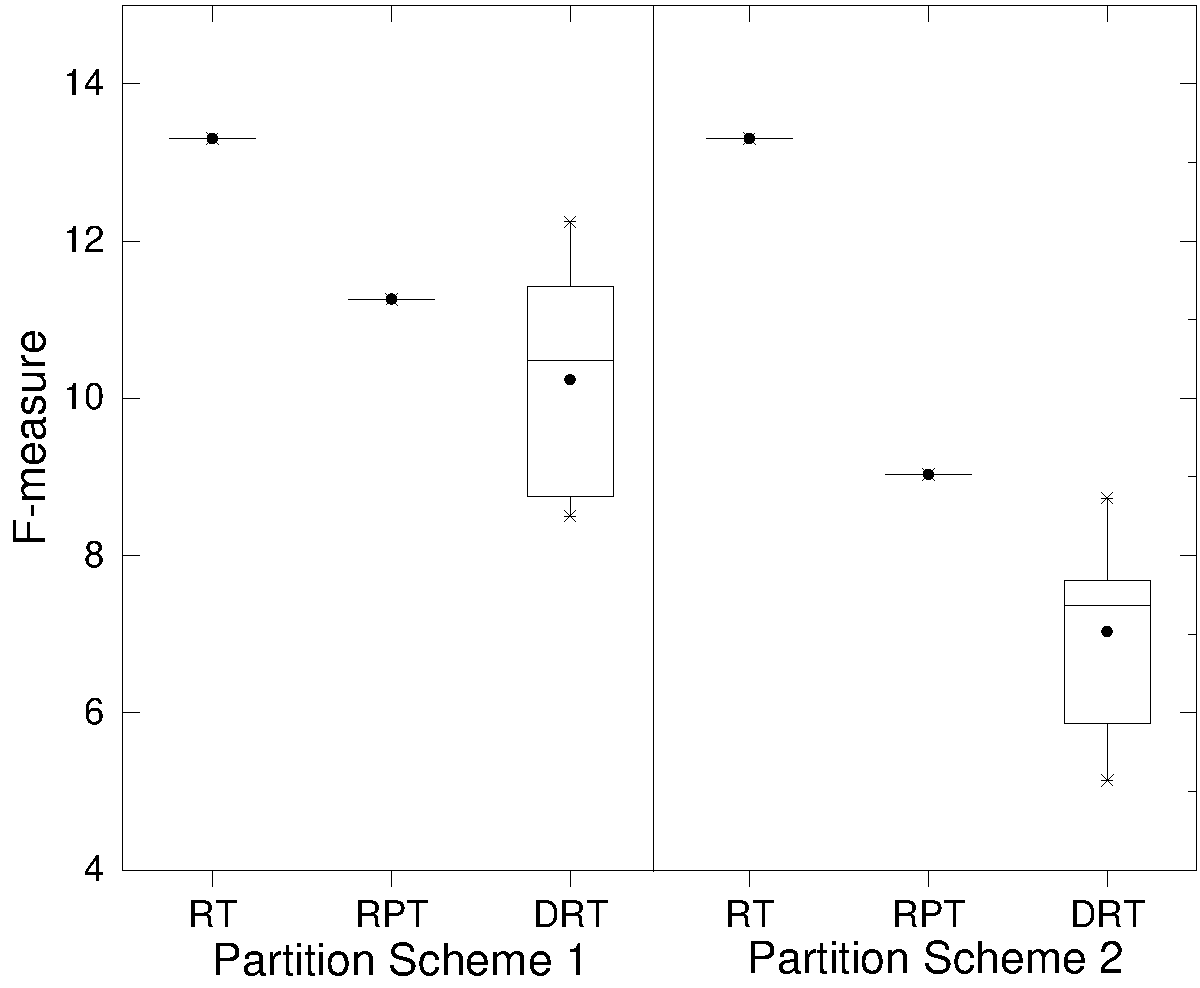
\includegraphics[width=0.32\textwidth,height=4cm]{fig/drtresultbox/aviaresultf.pdf}}
	\subfigure[CUBS] {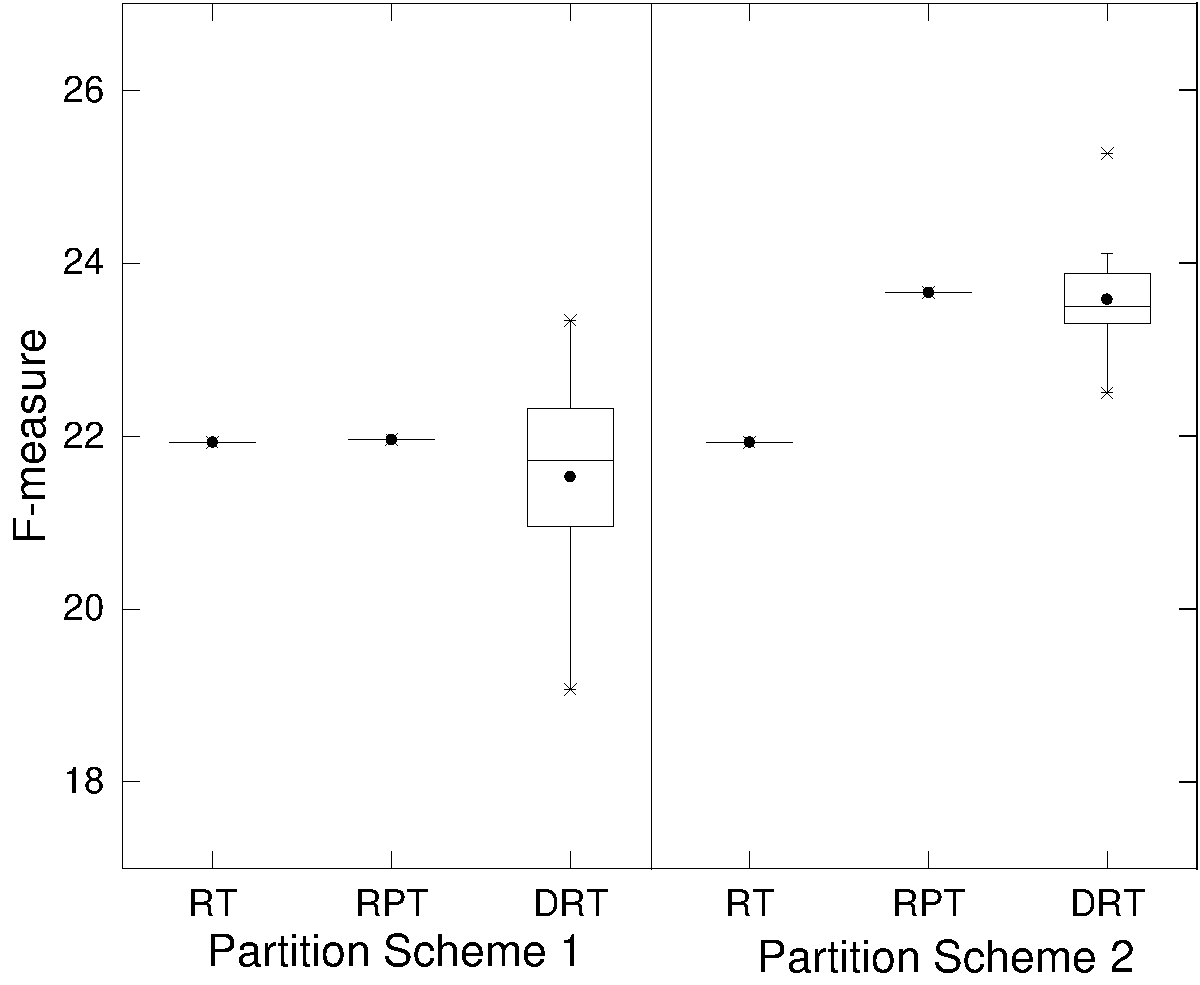
\includegraphics[width=0.32\textwidth,height=4cm]{fig/drtresultbox/chinaresultf.pdf}}
	\subfigure[PBS] {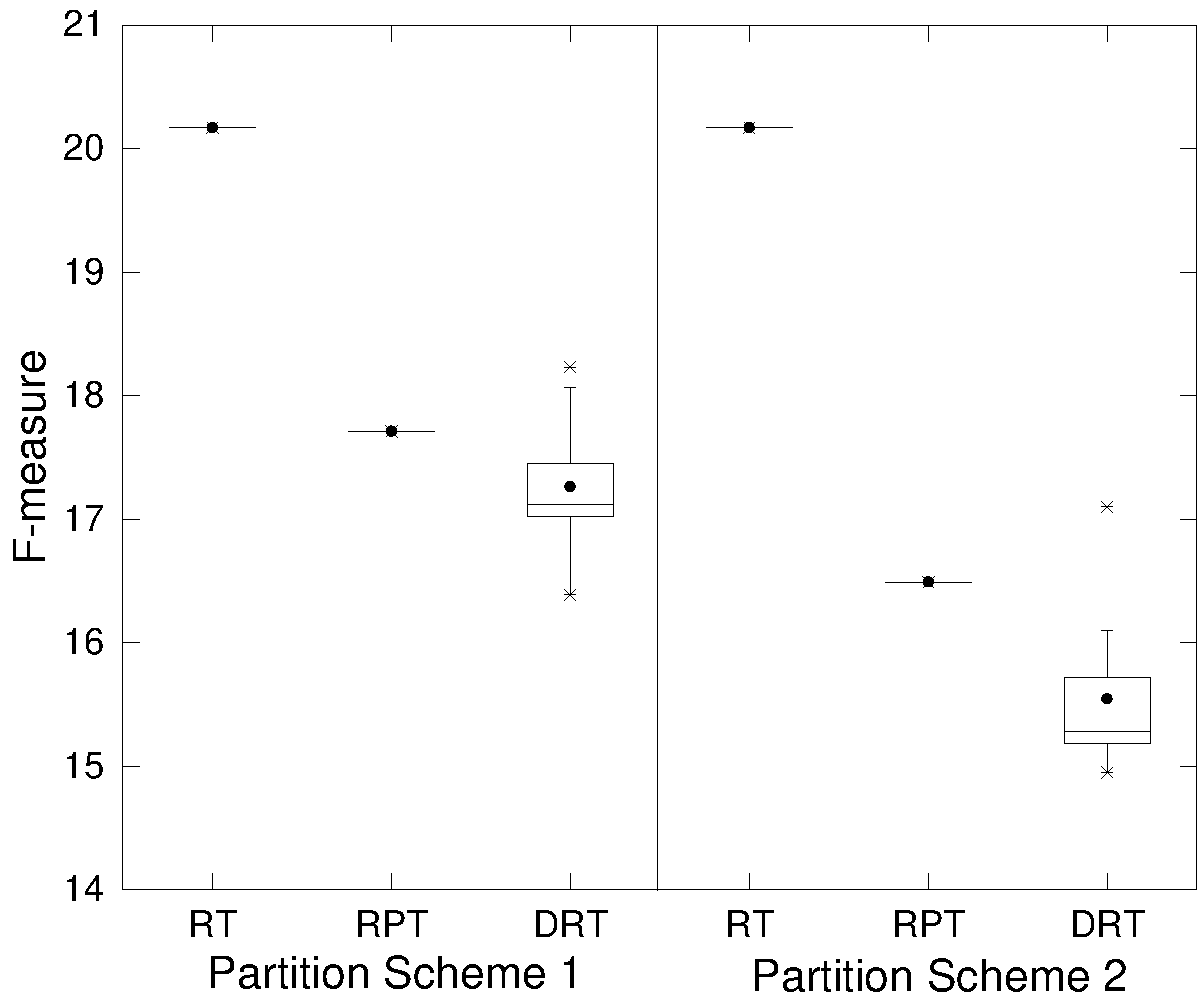
\includegraphics[width=0.32\textwidth,height=4cm]{fig/drtresultbox/parkingresultf.pdf}}
	\caption{F-measure boxplots for each program}
	\label{fig:Fmeasure}
\end{figure*}

\begin{figure*}
	\centering
	\subfigure[ACMS] {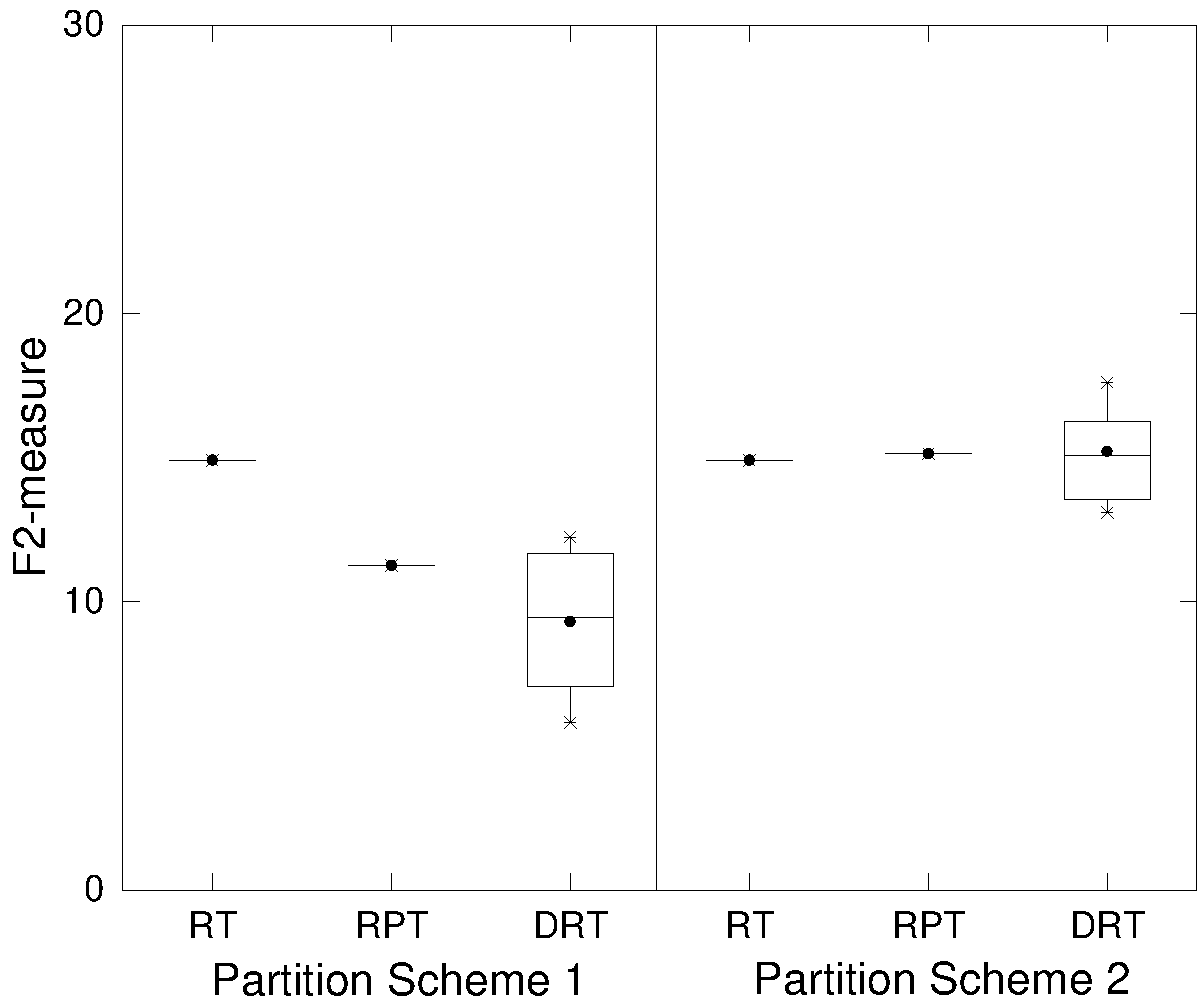
\includegraphics[width=0.32\textwidth,height=4cm]{fig/drtresultbox/aviaresultf2.pdf}}
	\subfigure[CUBS] {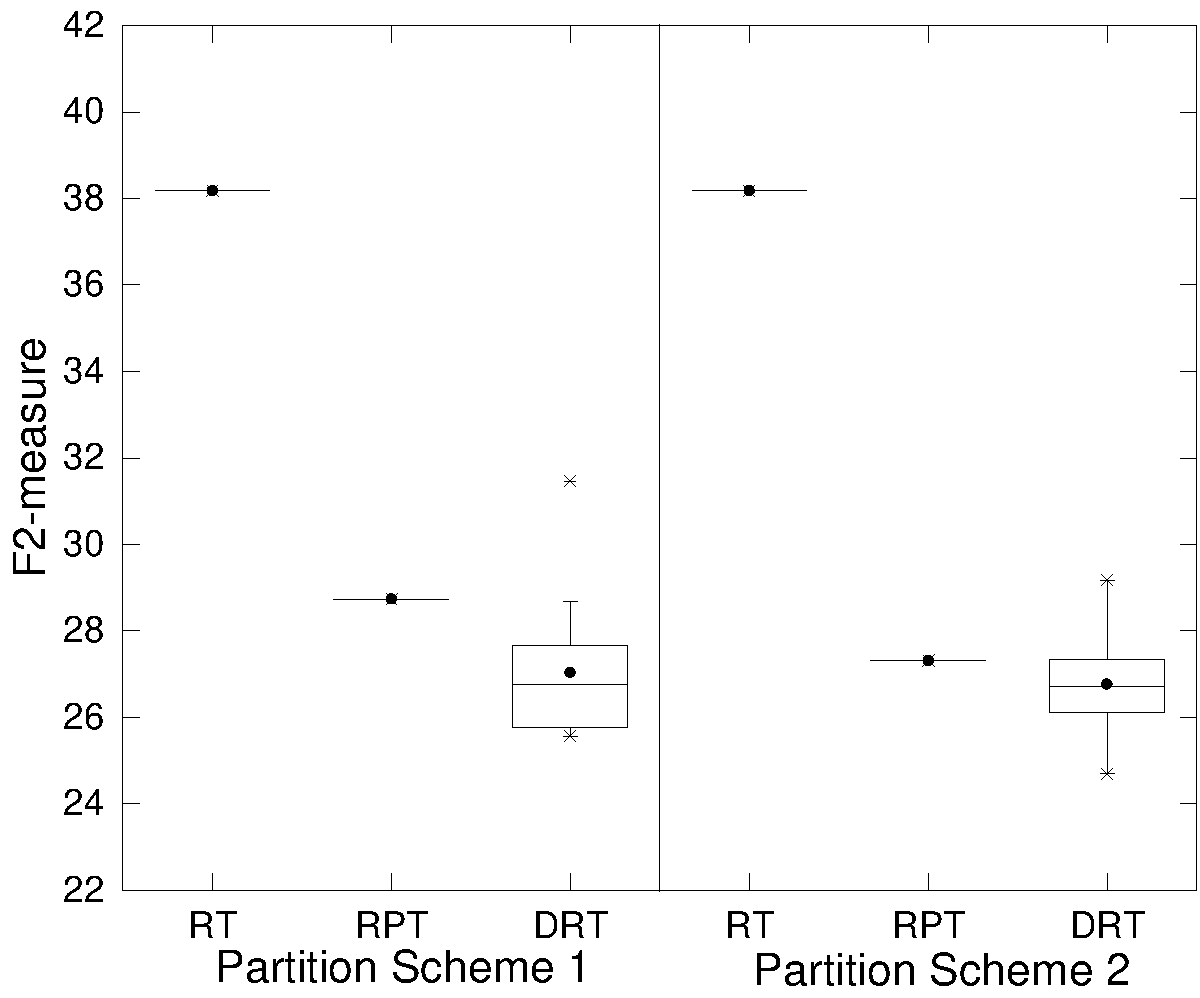
\includegraphics[width=0.32\textwidth,height=4cm]{fig/drtresultbox/chinaresultf2.pdf}}
	\subfigure[PBS] {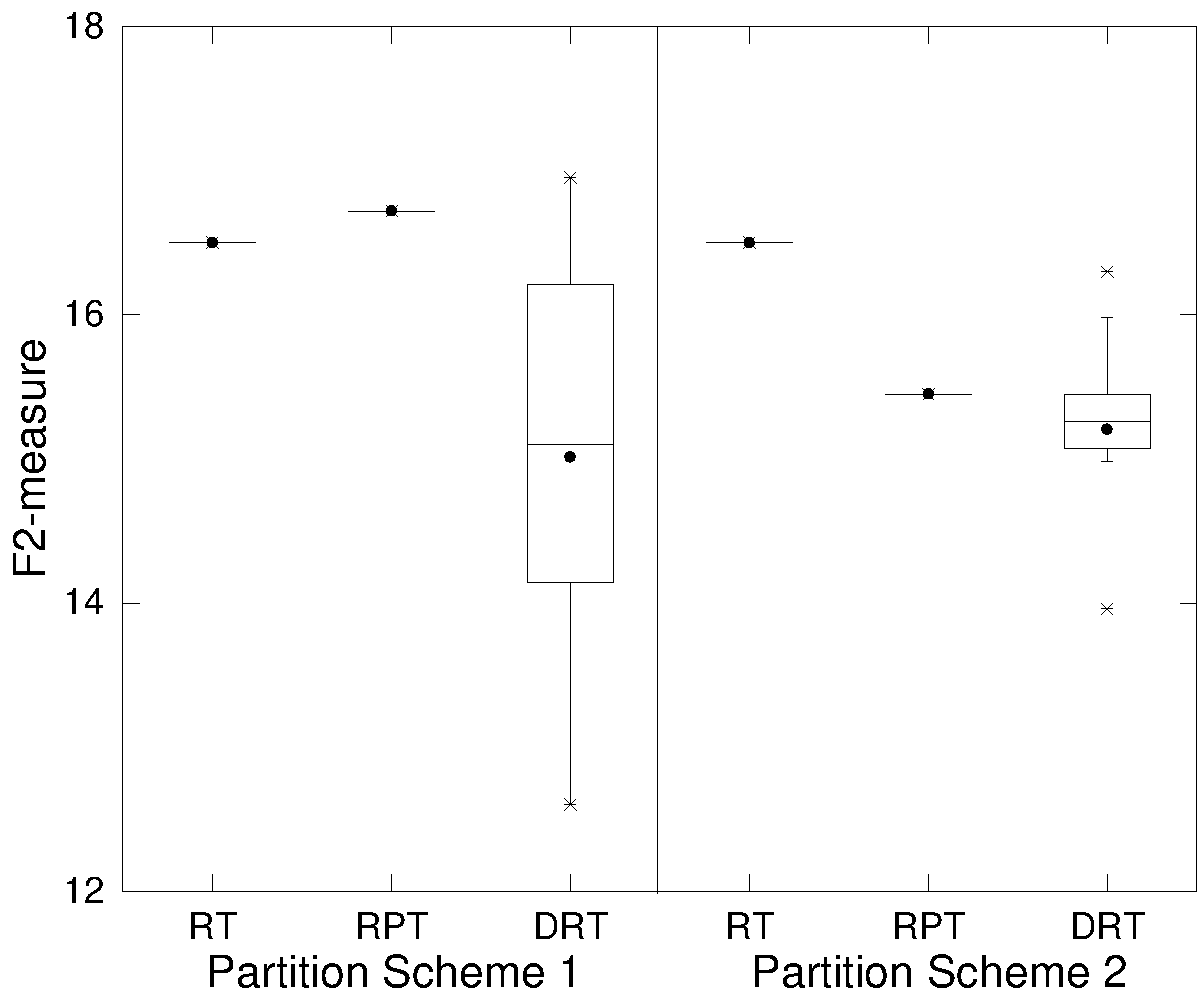
\includegraphics[width=0.32\textwidth,height=4cm]{fig/drtresultbox/parkingresultf2.pdf}}
	\caption{F2-measure boxplots for each program}
	\label{fig:F2measure}
\end{figure*}

\begin{figure*}
	\centering
	\subfigure[ACMS] {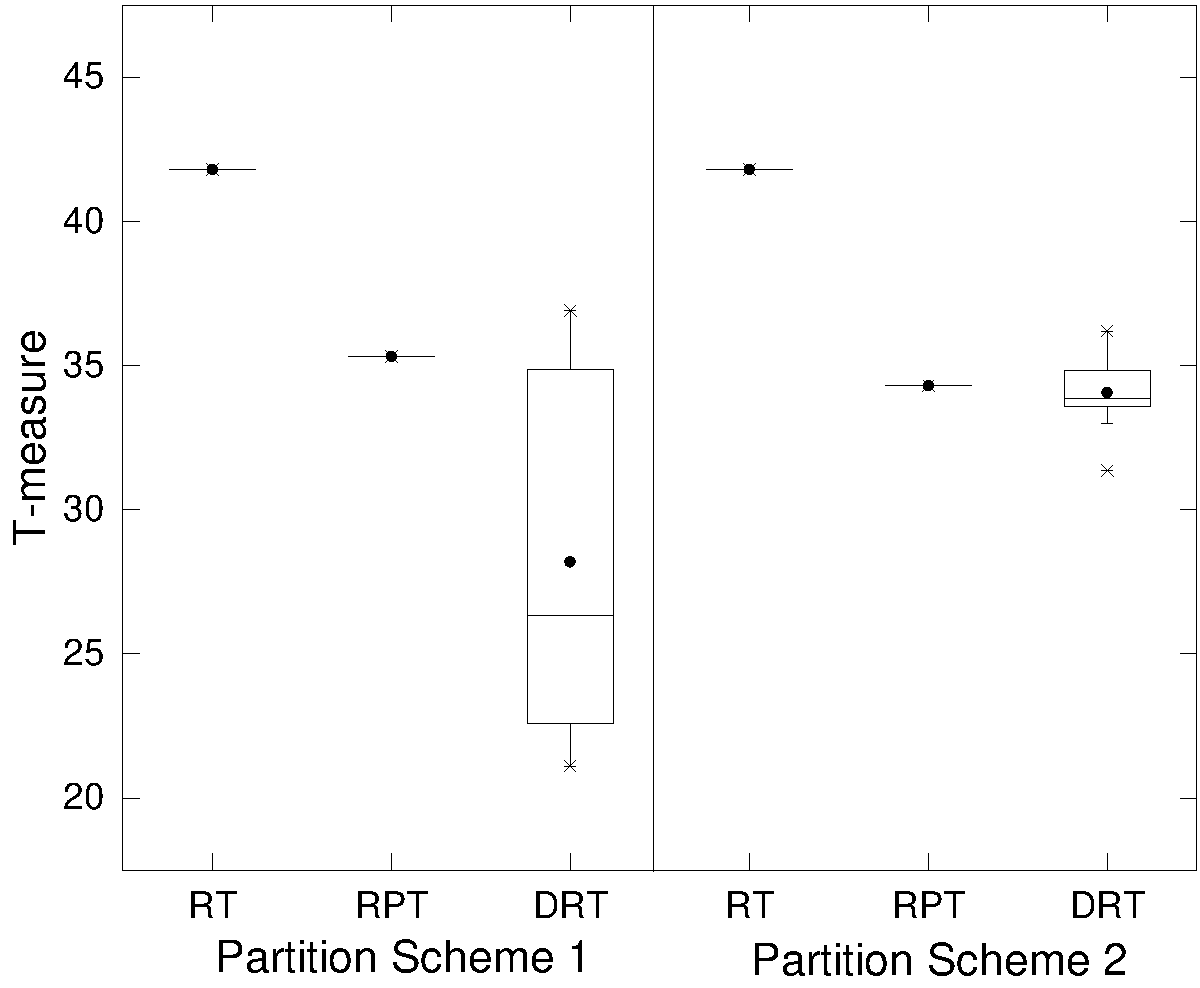
\includegraphics[width=0.32\textwidth,height=4cm]{fig/drtresultbox/aviaresultt.pdf}}
	\subfigure[CUBS] {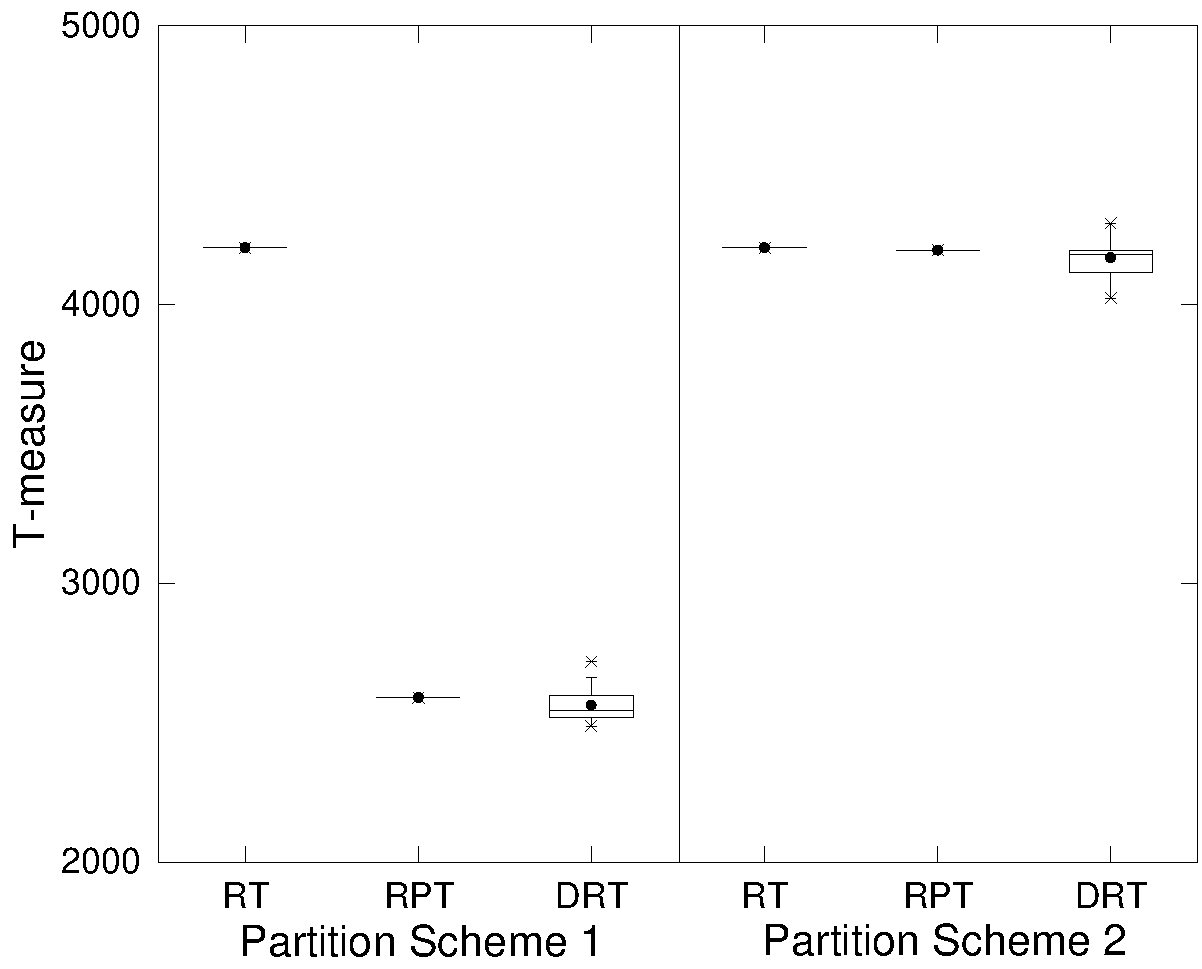
\includegraphics[width=0.32\textwidth,height=4cm]{fig/drtresultbox/chinaresultt.pdf}}
	\subfigure[PBS] {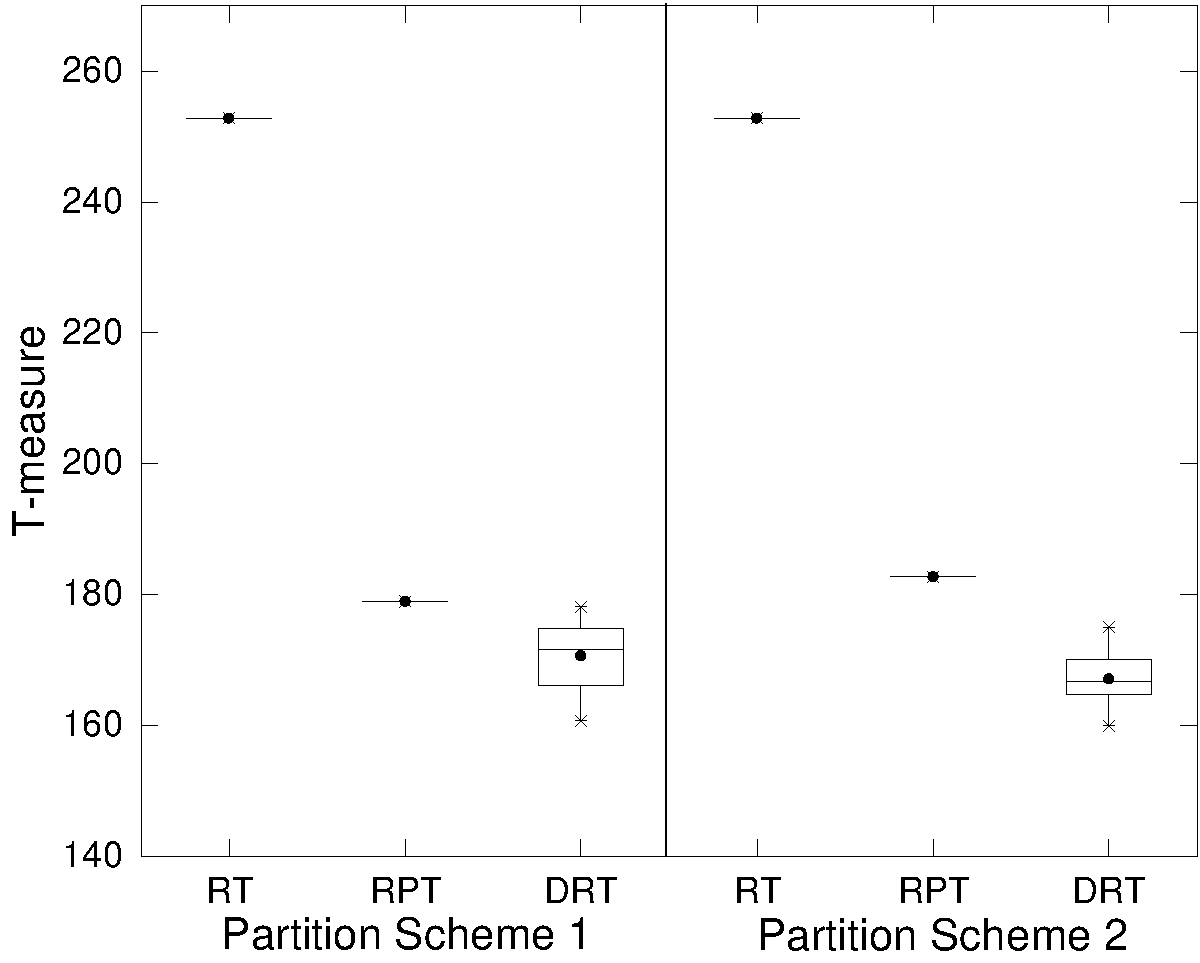
\includegraphics[width=0.32\textwidth,height=4cm]{fig/drtresultbox/parkingresultt.pdf}}
	\caption{T-measure boxplots for each program}
	\label{fig:Tmeasure}
\end{figure*}

It can observed from the tables and figures that, in general, DRT is the best performer, followed by RPT.
We also conducted statistical testing to verify the significance of this observation, using the Holm-Bonferroni method~\cite{sun2018adaptive} (with p-value equal to $0.05$) to determine which pairs of testing techniques had significant differences.
The statistical data are shown in Tables~\ref{tableHolm:fmeasure} to \ref{tableHlom:tmeasure}, where each cell gives the number of scenarios where the technique above (in the table) performed better than one to the left.
Where the difference is significant, the number is displayed in brackets. \dpt{perhaps we could consider a different way to indicate significance? brackets when not significant, or underlying when significant, for example. Bold is not so easy to see ...}
For example, the \underline{\textbf{75}} \dpt{this originally said 76. Please confirm that it should be 69}
in the top right cell of Table~\ref{tableHlom:tmeasure} indicates that, of 78 scenarios (13 parameters $\times$ tow partition schemes $\times$ three web services), DRT had lower F2-measure scores than RT for 75, with the fault-detection capabilities of these two techniques being significantly different.
\dpt{is ``scenarios'' correct?}

%From Tables~\ref{result:aviation} to~\ref{result:parking} and Figures~\ref{fig:Fmeasure} to \ref{fig:Tmeasure}, we can observe that in general, DRT was the best performer in terms of F-measure, F2-measure, and T-measure, followed by RPT. We further conducted statistical testing to verify the significance of this observation. We used the Holm-Bonferroni method~\cite{Holm79} (with p-value being 0.05) to determine which pairs of testing techniques have significant difference. The statistical testing results are shown in Tables~\ref{tableHolm:fmeasure},~\ref{tableHlom:nfmeasure} and~\ref{tableHlom:tmeasure}. Each cell in the tables gives the number of scenarios where the technique on the top row performed better than that on the left column. If the difference is significant, the number will be displayed in bold. For example, the bold 76 in the top right corner in Table~\ref{tableHlom:nfmeasure} indicates that out of 78 scenarios (13 parameters $\times$ 2 partition schemes $\times$ 3 object web services), DRT had smaller F2-measure than RT for 69 scenarios, and the fault-detection capabilities of these two techniques were significantly different.

\begin{table}[htbp]
  \caption{Number of Scenarios Where the Technique on the Top Row Has a Lower F-measure Score Than That on the Left Column}
  \centering
  \label{tableHolm:fmeasure}
  \begin{tabular}{|c|c|c|c|} \hline
          &RT         &RPT         &DRT                          \\ \hline
    RT    & ---       &4           &\underline{\textbf{60}}      \\ \hline
    RPT   &2          & ---        &\underline{\textbf{61}}      \\ \hline
    DRT   &18         &17          & ---        \\ \hline
  \end{tabular}
\end{table}

\begin{table}[htbp]
  \caption{Number of Scenarios Where the Technique on the Top Row Has a Lower F2-measure Score Than That on the Left Column}
  \centering
  \label{tableHlom:nfmeasure}
  \begin{tabular}{|c|c|c|c|} \hline
          &RT         &RPT              &DRT      \\ \hline
    RT    & ---       &4                &\underline{\textbf{69}}   \\ \hline
    RPT   &2          & ---             &\underline{\textbf{64}}   \\ \hline
    DRT   &9          &14               & ---     \\ \hline
  \end{tabular}
\end{table}

\begin{table}[htbp]
  \caption{Number of Scenarios Where the Technique on the Top Row Has a Lower T-measure Score Than That on the Left Column}
  \centering
  \label{tableHlom:tmeasure}
  \begin{tabular}{|c|c|c|c|} \hline
          &RT         &RPT         &DRT         \\ \hline
    RT    & ---       &6           &\underline{\textbf{75}}      \\ \hline
    RPT   &0          & ---        &\underline{\textbf{64}}       \\ \hline
    DRT   &3          &14          & ---         \\ \hline
  \end{tabular}
\end{table}


Tables~\ref{tableHolm:fmeasure} to \ref{tableHlom:tmeasure} clearly show that the difference between each pair of testing techniques is always significantly different.

\subsection{RQ2: Relationship between Partition Number and $\varepsilon$}

In~\ref{sec:relation}, we analyzed the relationship between the number of partitions and the DRT strategy parameter $\varepsilon$.
In this section, we show that our theoretical analysis provides useful guidance to testers to set the value of $\varepsilon$.

We used three web services to validate our theoretical analysis.
Before starting the test, the failure rate $\theta_i$ of partition $s_i$ was obtained by executing ($k$) test cases from $s_i$ until revealing a fault, then $\theta_i = k / k_i$, where $k_i$ is the total number of test cases in $s_i$.
According to Formula 19, the theoretically optimal values of~$\varepsilon$ in each scenario for each web service is shown in Table~\ref{tab:parameters}, where $\varepsilon^{*}$ denotes the theoretical value of $\varepsilon$. \dpt{why ``$h$''?}
We ran a series of experiments with the parameters set according to those in Table~\ref{tab:parameters}:
The F-, F2-, and T-measure results for each  program are shown in  Figure~\ref{fig:theovsnontheo}, where $\varepsilon_1^{*}$ and $\varepsilon_2^{*}$ denote the theoretically value of parameter $\varepsilon$ in different partition schemes, respectively. \dpt{why ``$h1$'' and ``$h2$''?}\dpt{it may be good to give some more explanation of the axes and values in Figure~\ref{fig:theovsnontheo}} \textcolor {red}{In order to make F-, F2-, and T-measure results easy to see and compare in Figure \ref{fig:theovsnontheo}, we make $log_{100}(1.0E05 \times \varepsilon)$ to be the value of the horizontal axis}.
Apart from the DRT strategy parameter $\varepsilon$, all other experimental settings remained the same as in Section~\ref{sec:1}.

\begin{table}
  \caption{Theoretical Optimal Values of DRT Parameter}
  \centering
  \label{tab:parameters}
  \begin{tabular}{|c|c|c|c|} \hline
     Web                         & Partition  &$\theta_{min}$   &$\varepsilon^{*}$             \\
     service                   & scheme     &                 &                \\ \hline
     \multirow{2}{*}{ACMS}       &1           &5.452E-2         &1.601E-1        \\ \cline{2-4}
                                 &2           &2.797E-3         &1.102E-4        \\ \hline
     \multirow{2}{*}{CUBS}       &1           &1.193E-3         &5.702E-5        \\ \cline{2-4}
                                 &2           &1.397E-3         &1.734E-5        \\ \hline
     \multirow{2}{*}{PBS}        &1           &1.760E-3         &1.118E-4        \\ \cline{2-4}
                                 &2           &1.492E-3         &1.340E-5        \\ \hline
  \end{tabular}
\end{table}

From Figure~\ref{fig:theovsnontheo}, we have the following observations:
\begin{itemize}
  \item
  In most scenarios, the DRT strategy with theoretically optimum parameter value performs best.
  Furthermore, the DRT strategy performs better when the parameter values are near the theoretically optimum value than when not.

  \item
  From Figure \ref{fig:theovsnontheo} (a), it can be observed that the DRT strategy with larger parameter values performs better than with the theoretically optimum value, in terms of the F-measure.
  The main reason for this is that, for this scenario, the maximum failure rate ($\theta_M = 4.781E-3$) is large and the number of partitions is small:
  When the parameter value is large, the probability of selecting partitions with lower failure rates is quickly reduced, and the probability of selecting partitions with larger failure rates is quickly increased, according to Formulas 3 and 4.
  \dpt{I'm not sure that I've captured the intended meaning in the paragraph/point above. Please check and confirm.}

\end{itemize}

\begin{figure*}
	\centering
    \subfigure[ACMS] {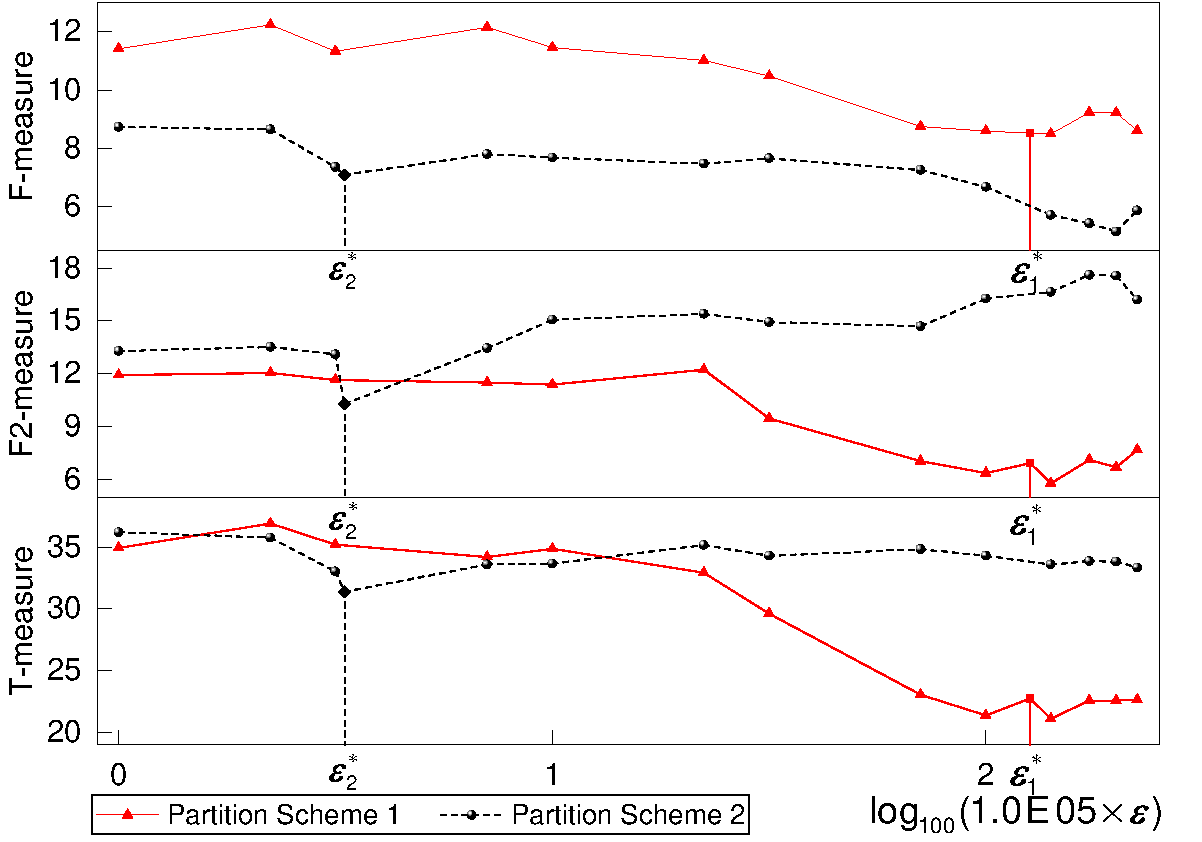
\includegraphics[width=0.32\textwidth,height=5cm]{fig/drtparemeter/avia.pdf}}
	\subfigure[CUBS] {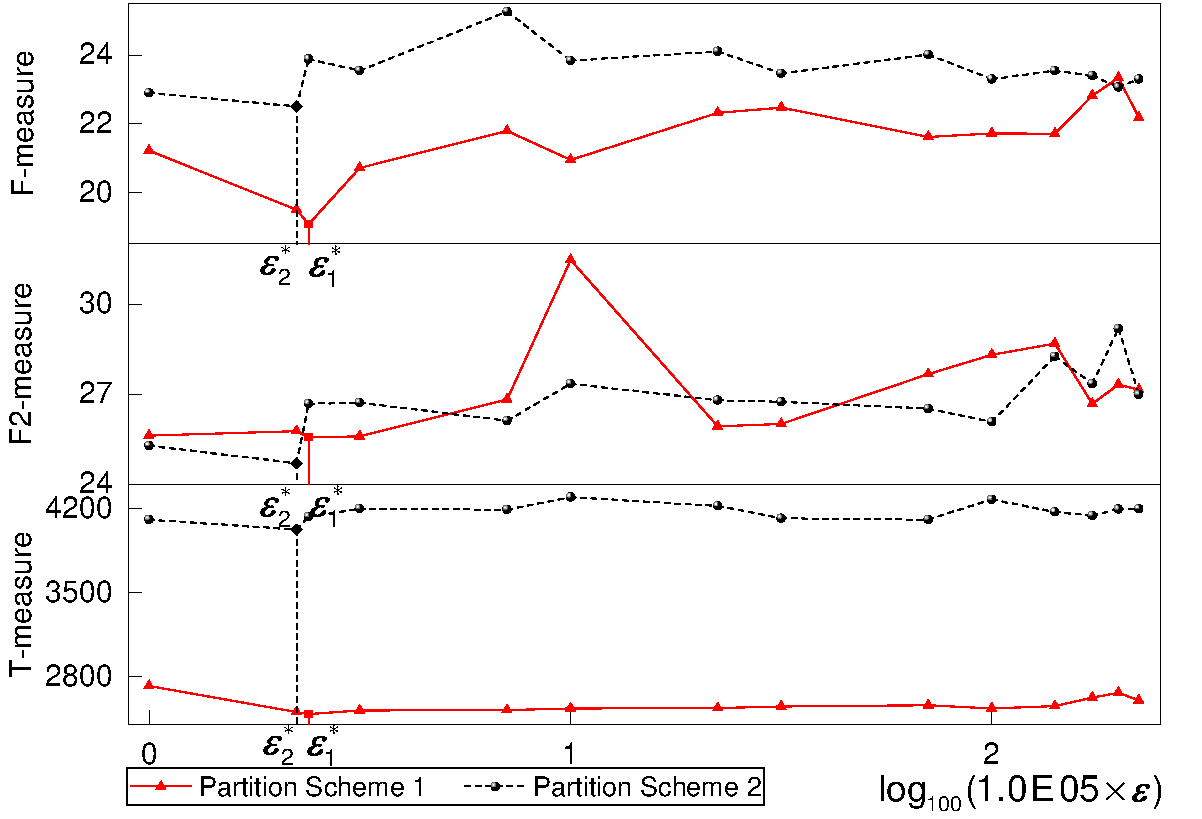
\includegraphics[width=0.32\textwidth,height=5cm]{fig/drtparemeter/china.pdf}}
	\subfigure[PBS] {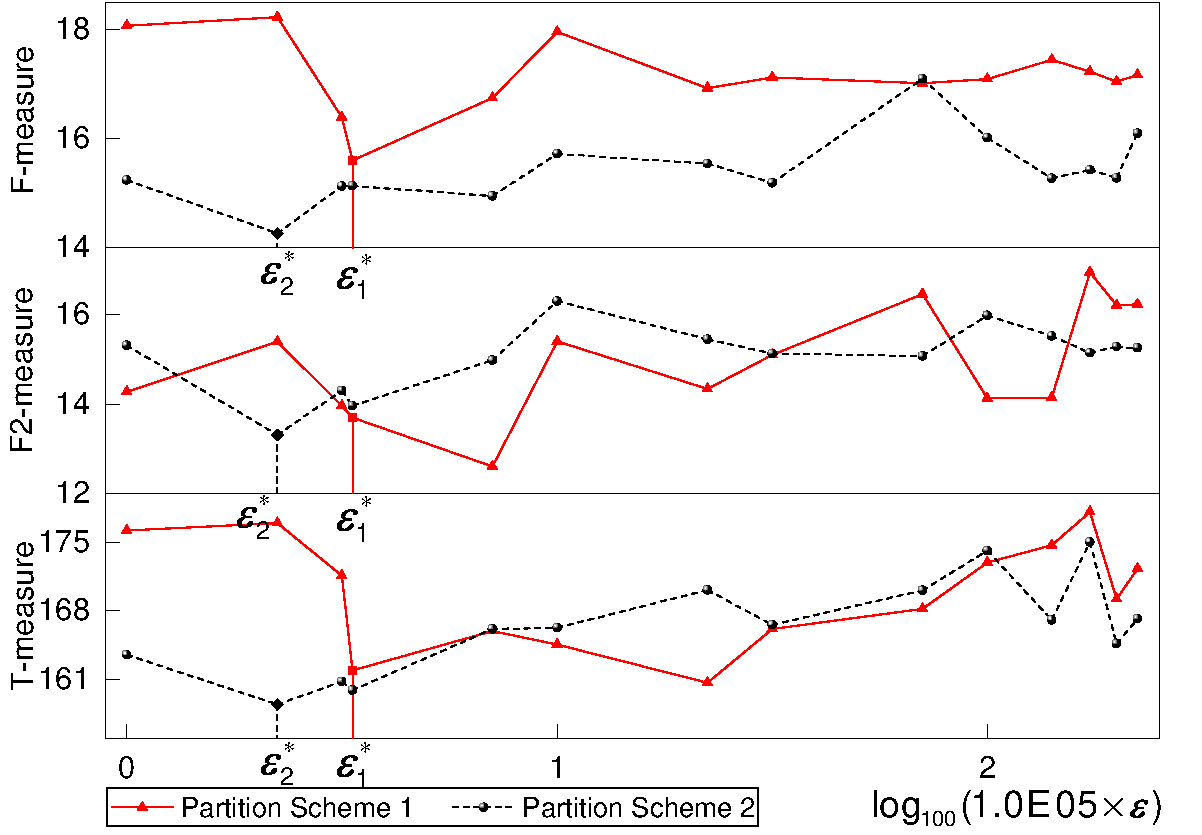
\includegraphics[width=0.32\textwidth,height=5cm]{fig/drtparemeter/parking.pdf}}
	\caption{Line charts of F-measure, F2-measure, and T-measure values for each program (for both the theoretically optimum parameter value, and other values}
	\label{fig:theovsnontheo}
\end{figure*}

%\begin{figure*}
%	\centering
%	\subfigure[ACMS] {\includegraphics[width=0.32\textwidth,height=4cm]{fig//f2aviavsnot}}
%	\subfigure[CUBS] {\includegraphics[width=0.32\textwidth,height=4cm]{fig//f2chinavsnot}}
%	\subfigure[PBS] {\includegraphics[width=0.32\textwidth,height=4cm]{fig//f2parkingvsnot}}
%	\caption{Boxplots of F2-measure on each object program with theoretical parameter}
%	\label{fig:F2theovs}
%\end{figure*}
%
%\begin{figure*}
%	\centering
%	\subfigure[ACMS] {\includegraphics[width=0.32\textwidth,height=4cm]{fig//taviavsnot}}
%	\subfigure[CUBS] {\includegraphics[width=0.32\textwidth,height=4cm]{fig//tchinavsnot}}
%	\subfigure[PBS] {\includegraphics[width=0.32\textwidth,height=4cm]{fig//tparkingvsnot}}
%	\caption{Boxplots of T-measure on each object program with theoretical parameter}
%	\label{fig:Ttheovs}
%\end{figure*}

\subsection{RQ3: Selection Overhead}

Tables~\ref{tab:timeavia} to~\ref{tab:timeparking} summarize the F-, F2-, and T-time results, respectively, and their distributions for each web service is shown in Figures~\ref{fig:Ftime} to \ref{fig:Ttime}. \dpt{These figures don't say Scheme/a 1 or 2...}
It can be observed from the figures that, in general, DRT had the best performance, and RPT just marginally outperforms RT.

\begin{table}[!hbt]
  \caption{F-time, F2-time and T-time for Web Service ACMS (in ms)}
  \label{tab:timeavia}
  \centering
  \setlength{\tabcolsep}{1mm}{
  \begin{tabular}{|c|c|c|c|c|c|c|c|} \hline
     \multicolumn{2}{|c|}{\multirow{2}{*}{Strategy}} &\multicolumn{3}{|c|}{Partition scheme 1} &\multicolumn{3}{|c|}{Partition scheme 2}\\ \cline{3-8}
     \multicolumn{2}{|c|}{}    &F-time	&F2-time &T-time &F-time &F2-time &T-time  \\ \hline
     \multicolumn{2}{|c|}{RT}  &0.43	&0.29	&0.85	&0.43 	&0.29	&0.85   \\ \hline
     \multicolumn{2}{|c|}{RPT} &0.57	&0.31	&1.08	&0.33	&0.45	&0.78   \\ \hline
         \multirow{13}{*}{DRT} &1.0E-5    &0.47	&0.28	&0.96	&0.38	&0.41	&0.95  \\ \cline{2-8}
                               &5.0E-5	  &0.35	&0.21	&0.78	&0.30	&0.27	&0.71 \\ \cline{2-8}
                               &1.0E-4	  &0.33	&0.19	&0.66	&0.24	&0.28	&0.65 \\ \cline{2-8}
                               &5.0E-4	  &0.30	&0.17	&0.60	&0.27	&0.25	&0.67 \\ \cline{2-8}
                               &1.0E-3	  &0.29	&0.19	&0.61	&0.22	&0.24	&0.60 \\ \cline{2-8}
                               &5.0E-3	  &0.28	&0.23	&0.62	&0.21	&0.31	&0.64 \\ \cline{2-8}
                               &1.0E-2	  &0.24	&0.17	&0.53	&0.23	&0.29	&0.66 \\ \cline{2-8}
                               &5.0E-2	  &0.28	&0.13	&0.49	&0.23	&0.35	&0.71 \\ \cline{2-8}
                               &1.0E-1	  &0.26	&0.08	&0.43	&0.23	&0.29	&0.63 \\ \cline{2-8}
                               &2.0E-1	  &0.23	&0.12	&0.43	&0.30	&0.46	&0.89 \\ \cline{2-8}
                               &3.0E-1	  &0.24	&0.11	&0.45	&0.18	&0.40	&0.69 \\ \cline{2-8}
                               &4.0E-1	  &0.27	&0.10	&0.47	&0.16	&0.31	&0.58 \\ \cline{2-8}
                               &5.0E-1	  &0.28	&0.11	&0.47	&0.28	&0.45	&0.86 \\ \hline
  \end{tabular}}
\end{table}


\begin{table}[!hbt]
  \caption{F-time, F2-time and T-time for Web Service CUBS (in ms)}
  \label{tab:timechina}
  \centering
  \setlength{\tabcolsep}{1mm}{
  \begin{tabular}{|c|c|c|c|c|c|c|c|} \hline
     \multicolumn{2}{|c|}{\multirow{2}{*}{Strategy}} &\multicolumn{3}{|c|}{Partition scheme 1} &\multicolumn{3}{|c|}{Partition scheme 2}\\ \cline{3-8}
     \multicolumn{2}{|c|}{}    &F-time	&F2-time &T-time &F-time &F2-time &T-time  \\ \hline
     \multicolumn{2}{|c|}{RT}  &0.82	&1.14	&34.69	&0.82	&1.14	&34.69   \\ \hline
     \multicolumn{2}{|c|}{RPT} &0.91	&0.87	&30.54	&0.75	&0.79	&34.59   \\ \hline
         \multirow{13}{*}{DRT} &1.0E-5    &0.91	&0.87	&30.14	&0.87	&0.83	&36.49  \\ \cline{2-8}
                               &5.0E-5	  &0.95	&0.86	&30.21	&0.82	&0.75	&34.7\\ \cline{2-8}
                               &1.0E-4	  &0.77	&0.89	&29.27	&0.86	&0.69	&35.34 \\ \cline{2-8}
                               &5.0E-4	  &0.79	&1.00	&31.05	&0.87	&0.90	&36.85 \\ \cline{2-8}
                               &1.0E-3	  &0.86	&0.88	&29.93	&0.92	&0.77	&36.44 \\ \cline{2-8}
                               &5.0E-3	  &0.86	&0.83	&30.28	&0.83	&0.83	&36.27 \\ \cline{2-8}
                               &1.0E-2	  &0.95	&0.88	&29.33	&0.84	&0.72	&35.23 \\ \cline{2-8}
                               &5.0E-2	  &0.84	&0.82	&30.56	&0.88	&0.72	&37.07 \\ \cline{2-8}
                               &1.0E-1	  &0.88	&0.93	&29.45	&0.82	&0.76	&37.14 \\ \cline{2-8}
                               &2.0E-1	  &0.83	&0.83	&30.16	&0.86	&0.73	&36.79 \\ \cline{2-8}
                               &3.0E-1	  &0.95	&0.86	&27.81	&0.84	&0.84	&36.89 \\ \cline{2-8}
                               &4.0E-1	  &0.84	&0.84	&28.23	&0.86	&0.82	&35.22 \\ \cline{2-8}
                               &5.0E-1	  &0.87	&0.84	&27.91	&0.90	&0.86	&38.21 \\ \hline
  \end{tabular}}
\end{table}

\begin{table}[!hbt]
  \caption{F-time, F2-time and T-time for Web Service PBS (in ms)}
  \label{tab:timeparking}
  \centering
  \setlength{\tabcolsep}{1mm}{
  \begin{tabular}{|c|c|c|c|c|c|c|c|} \hline
     \multicolumn{2}{|c|}{\multirow{2}{*}{Strategy}} &\multicolumn{3}{|c|}{Partition scheme 1} &\multicolumn{3}{|c|}{Partition scheme 2}\\ \cline{3-8}
     \multicolumn{2}{|c|}{}    &F-time	&F2-time &T-time &F-time &F2-time &T-time  \\ \hline
     \multicolumn{2}{|c|}{RT}  &0.81	&0.42	&4.12	&0.81	&0.42	&4.12   \\ \hline
     \multicolumn{2}{|c|}{RPT} &0.85	&0.52	&3.83	&0.66	&0.35	&2.98   \\ \hline
         \multirow{13}{*}{DRT} &1.0E-5    &0.76	&0.48	&3.85	&1.05	&0.51	&3.44  \\ \cline{2-8}
                               &5.0E-5    &0.73	&0.35	&3.02	&0.91	&0.52	&3.79\\ \cline{2-8}
                               &1.0E-4    &0.54	&0.36	&2.97	&0.49	&0.34	&2.26 \\ \cline{2-8}
                               &5.0E-4    &0.68	&0.34	&3.20	&0.50	&0.30	&2.31 \\ \cline{2-8}
                               &1.0E-3    &0.62	&0.38	&2.87	&0.52	&0.38	&2.42 \\ \cline{2-8}
                               &5.0E-3    &0.60	&0.38	&2.99	&0.43	&0.51	&2.40 \\ \cline{2-8}
                               &1.0E-2    &0.58	&0.42	&2.84	&0.51	&0.34	&2.41 \\ \cline{2-8}
                               &5.0E-2    &0.64	&0.44	&3.27	&0.59	&0.36	&2.49 \\ \cline{2-8}
                               &1.0E-1    &0.65	&0.38	&3.46	&0.60	&0.38	&2.56 \\ \cline{2-8}
                               &2.0E-1	  &0.60	&0.36	&3.22	&0.54	&0.59	&2.47 \\ \cline{2-8}
                               &3.0E-1	  &0.59	&0.44	&3.24	&0.57	&0.46	&2.57 \\ \cline{2-8}
                               &4.0E-1	  &0.61	&0.33	&2.90	&0.51	&0.33	&2.54 \\ \cline{2-8}
                               &5.0E-1	  &0.62	&0.44	&3.16	&0.56	&0.36	&2.56 \\ \hline
  \end{tabular}}
\end{table}

\begin{figure*}
	\centering
    \subfigure[ACMS] {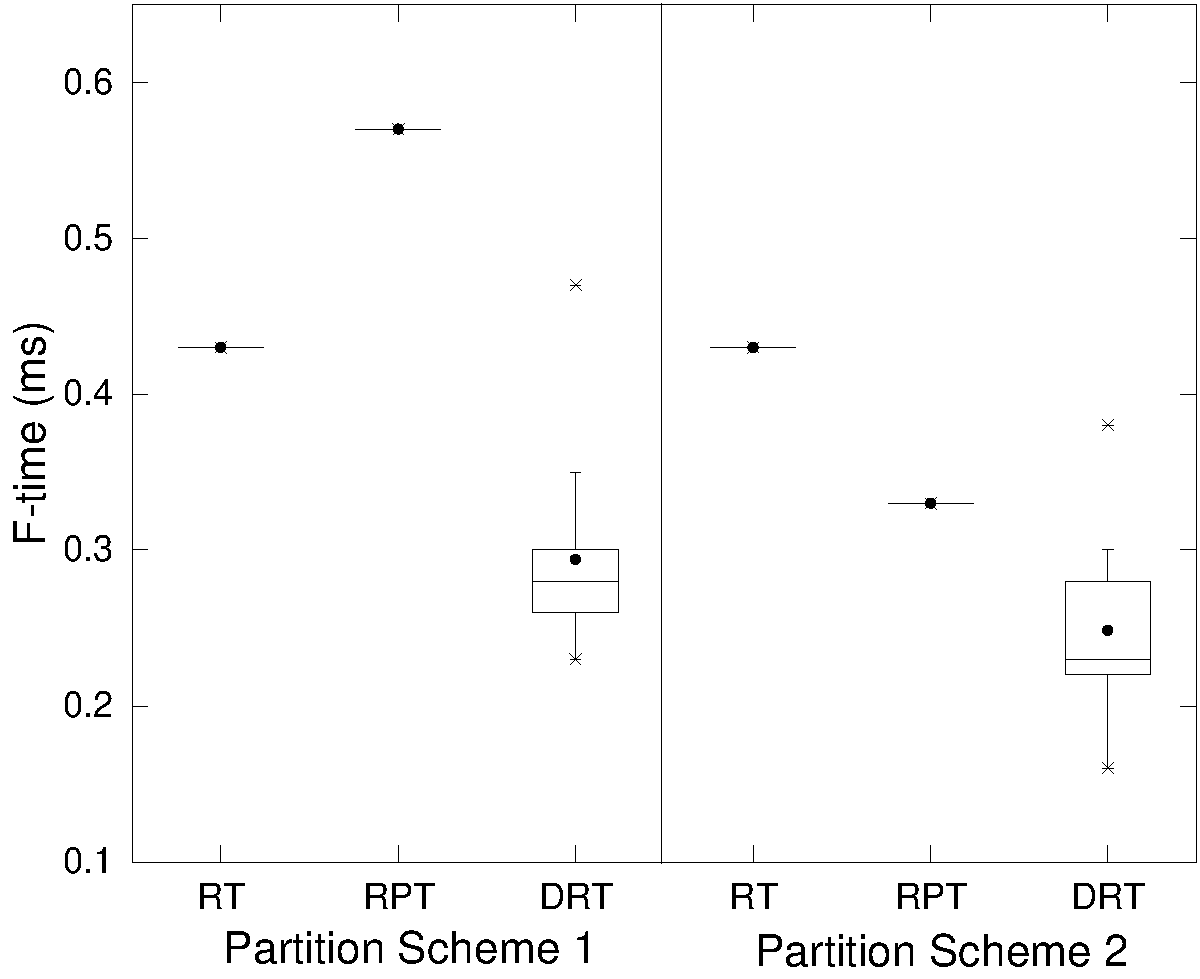
\includegraphics[width=0.32\textwidth,height=4cm]{fig/drttime/aviatimef}}
	\subfigure[CUBS] {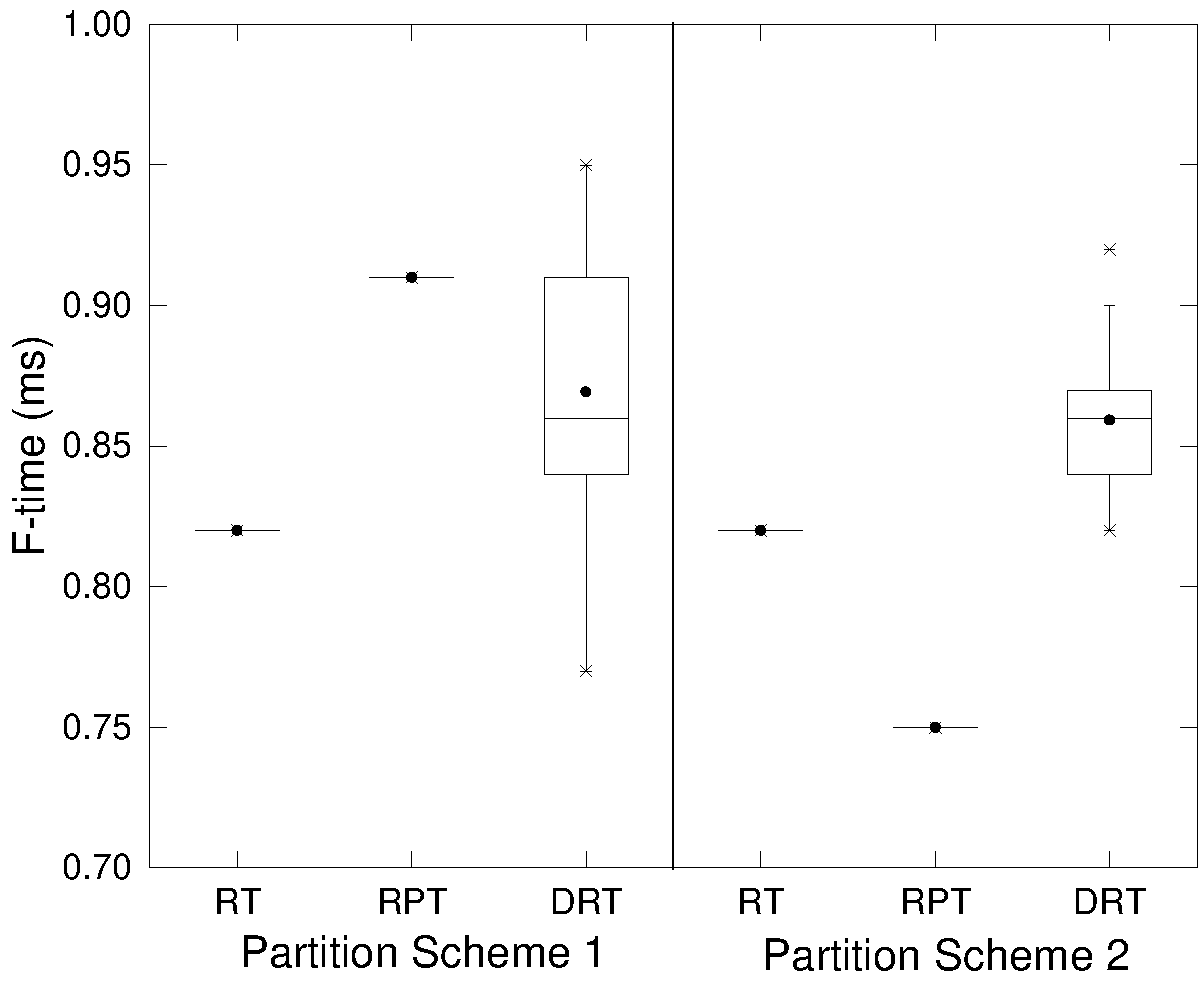
\includegraphics[width=0.32\textwidth,height=4cm]{fig/drttime/chinatimef}}
	\subfigure[PBS] {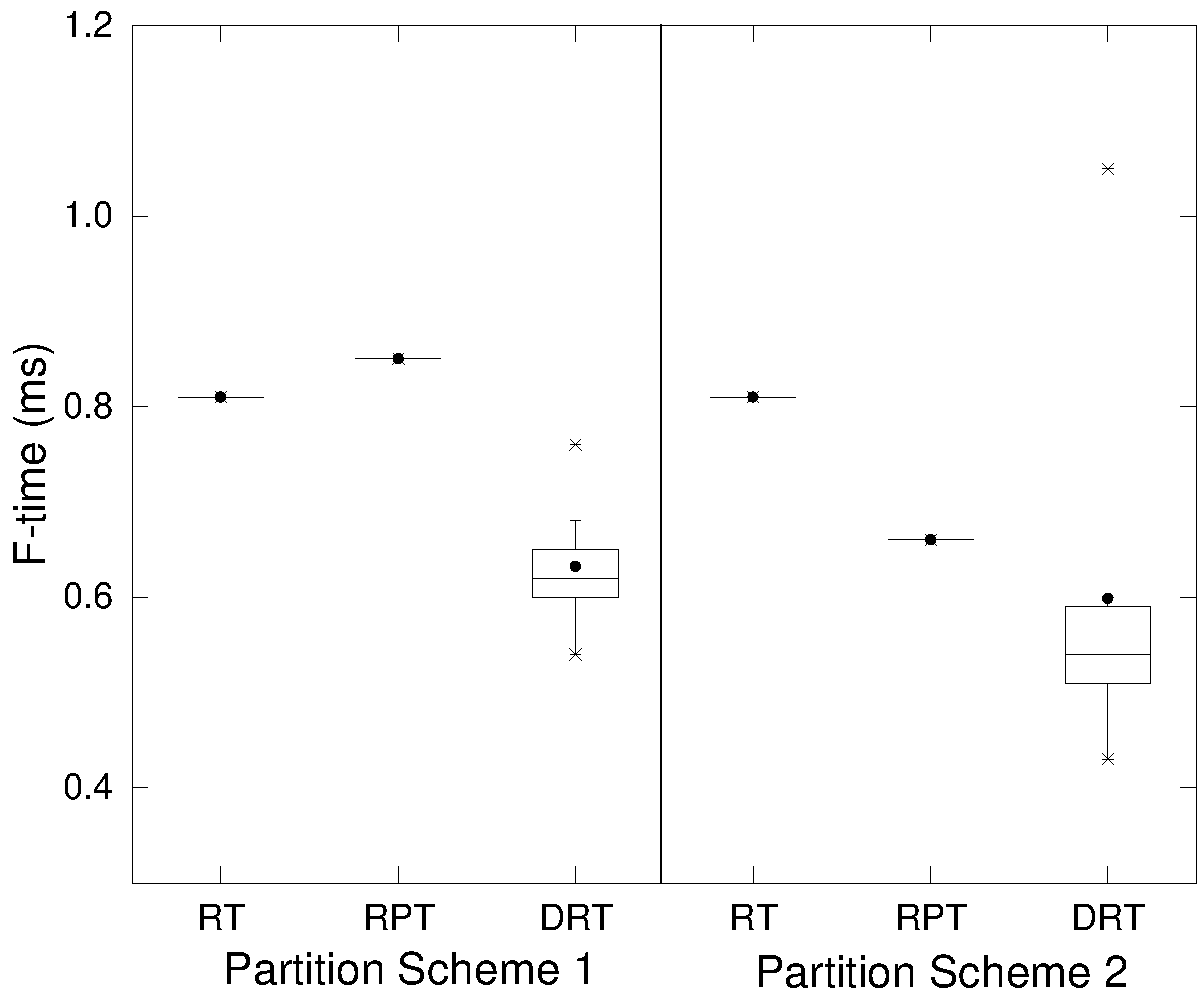
\includegraphics[width=0.32\textwidth,height=4cm]{fig/drttime/parkingtimef}}
	\caption{F-time boxplots for each program}
	\label{fig:Ftime}
\end{figure*}

\begin{figure*}
	\centering
	\subfigure[ACMS] {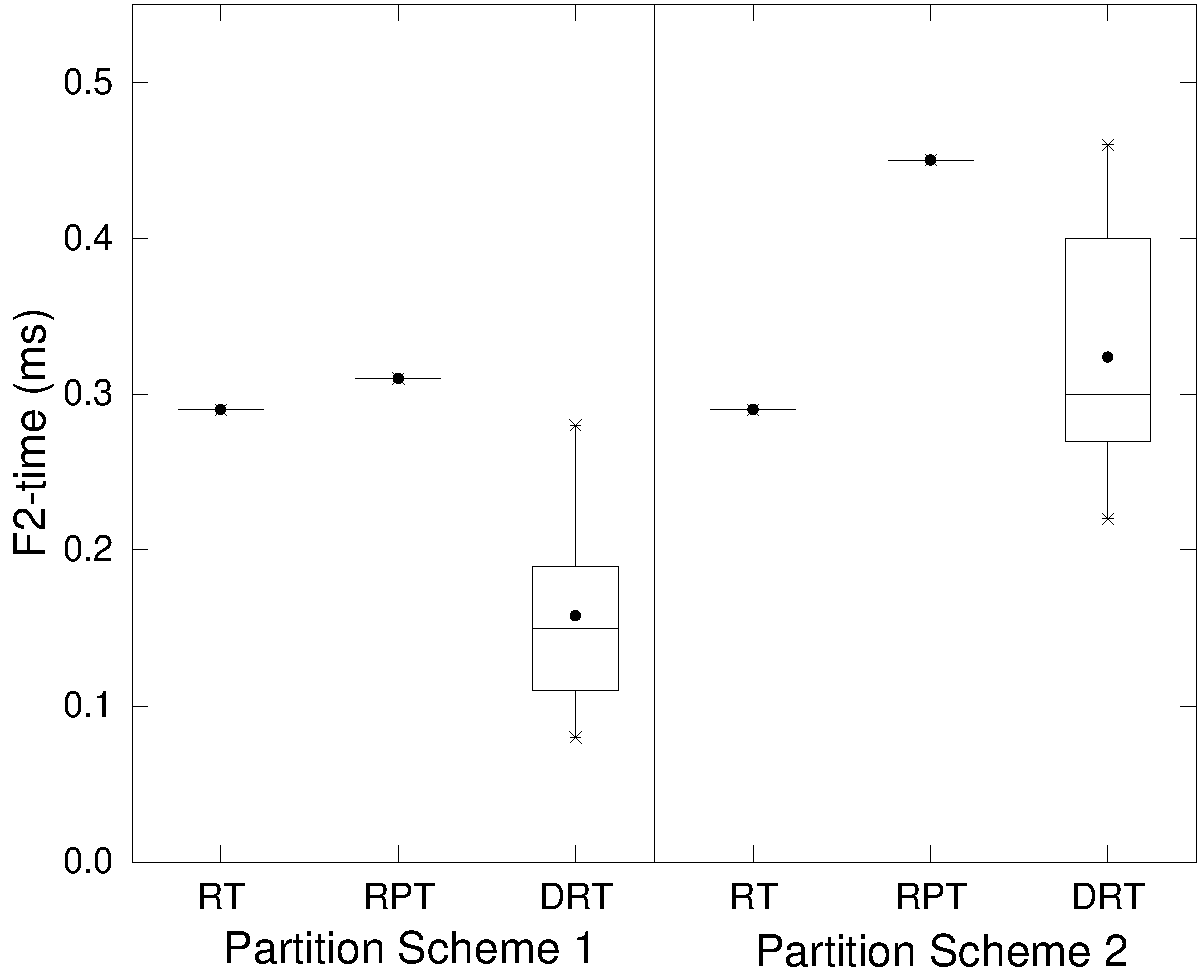
\includegraphics[width=0.32\textwidth,height=4cm]{fig/drttime/aviatimef2}}
	\subfigure[CUBS] {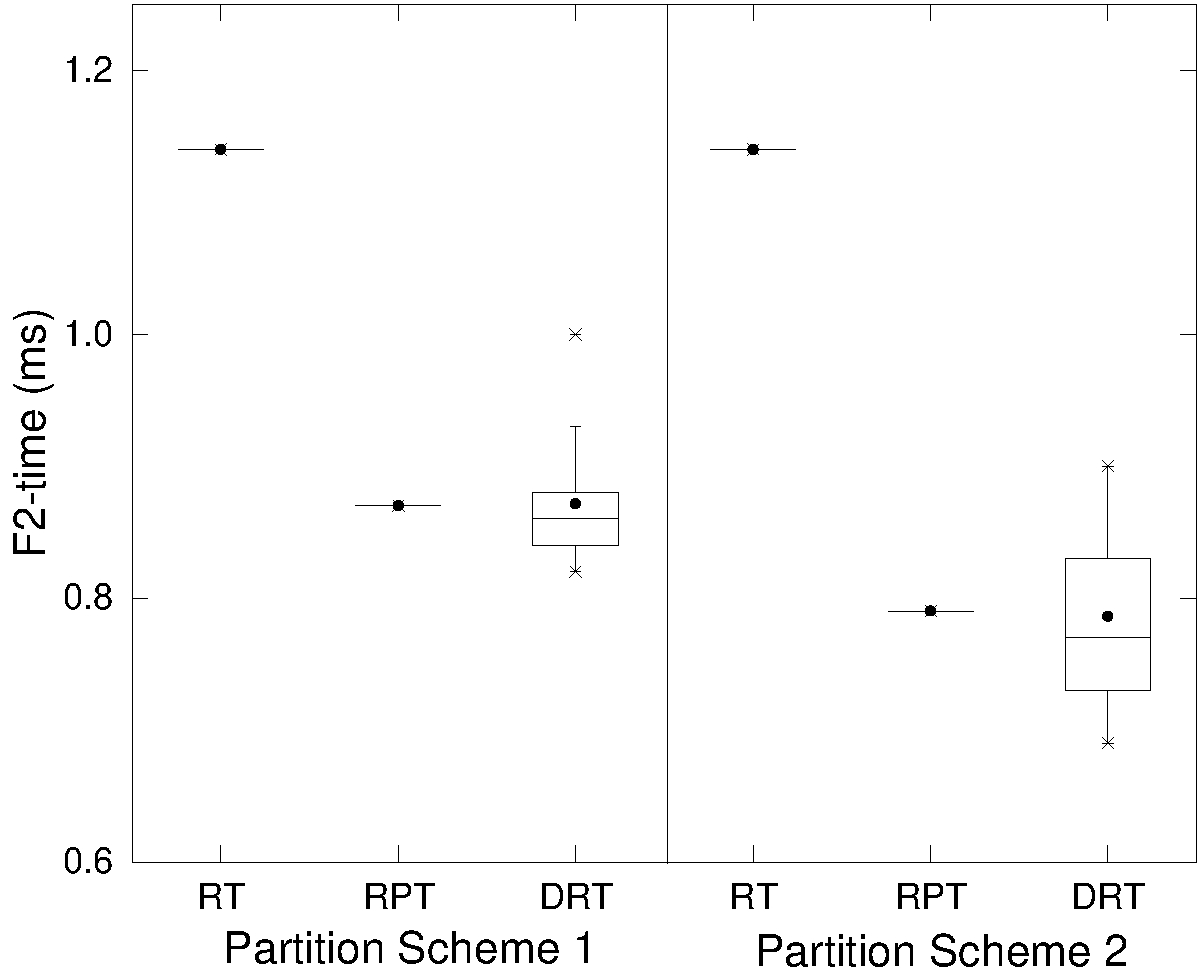
\includegraphics[width=0.32\textwidth,height=4cm]{fig/drttime/chinatimef2}}
	\subfigure[PBS] {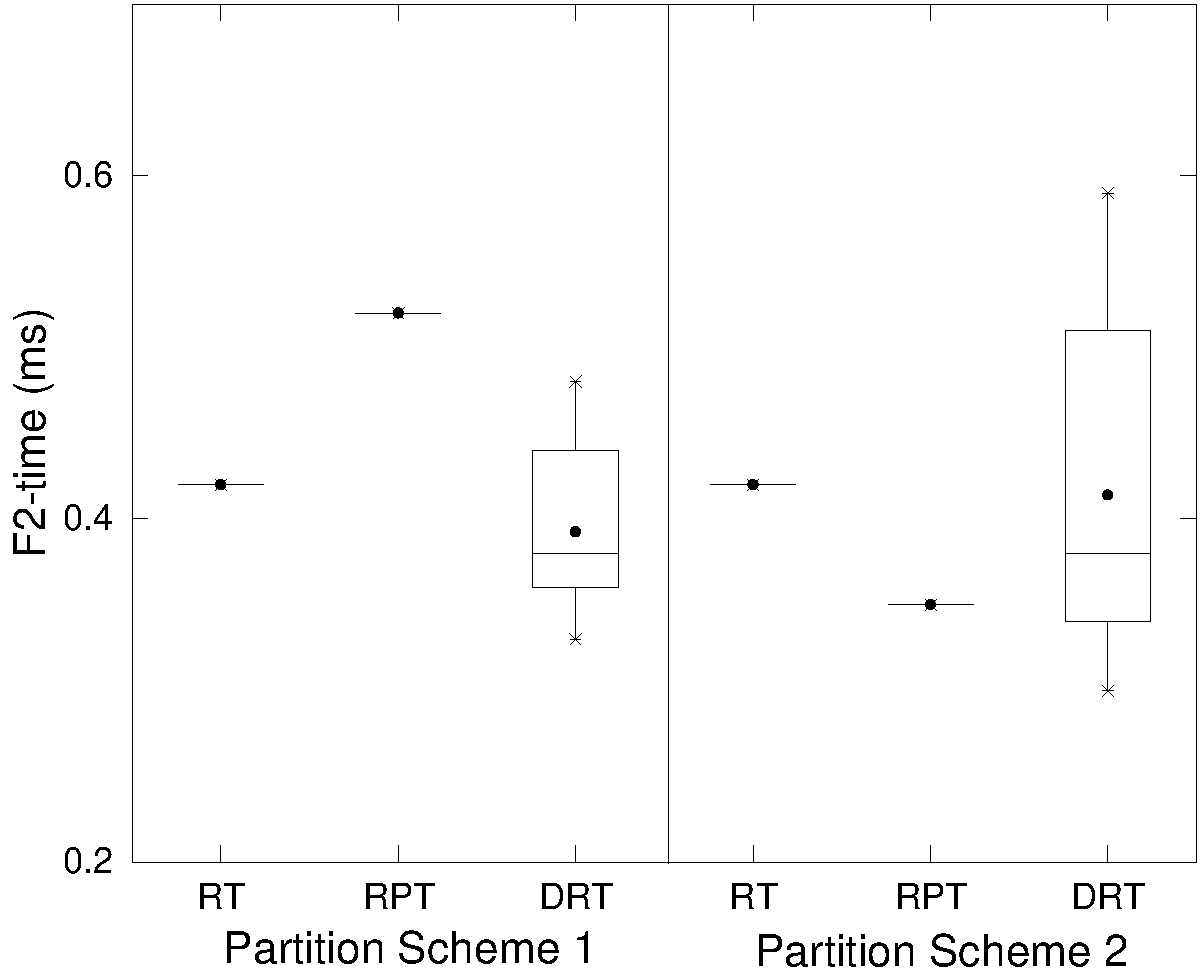
\includegraphics[width=0.32\textwidth,height=4cm]{fig/drttime/parkingtimef2}}
	\caption{F2-time boxplots for each program}
	\label{fig:F2time}
\end{figure*}


\begin{figure*}
	\centering
	\subfigure[ACMS] {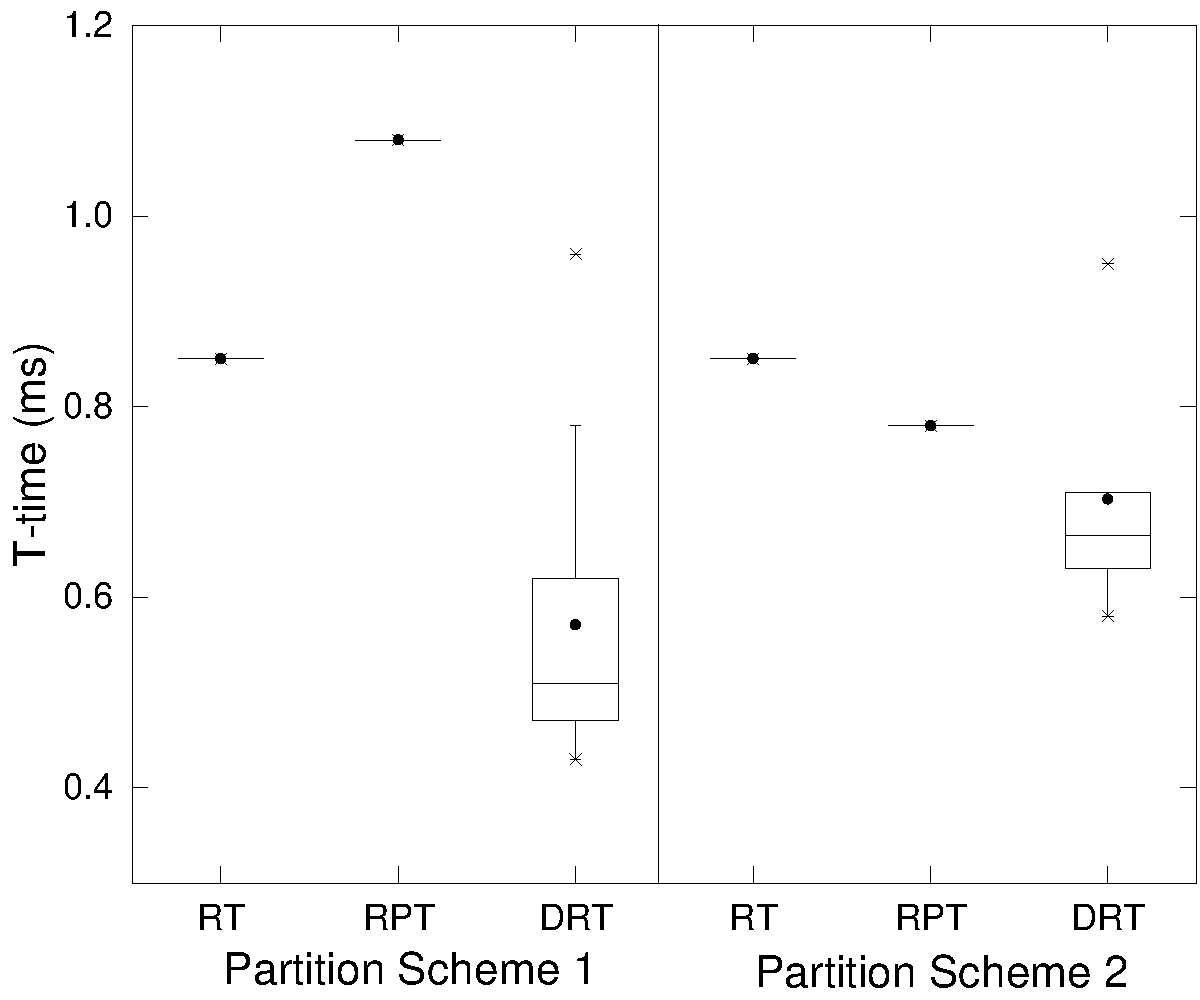
\includegraphics[width=0.32\textwidth,height=4cm]{fig/drttime/aviatimet}}
	\subfigure[CUBS] {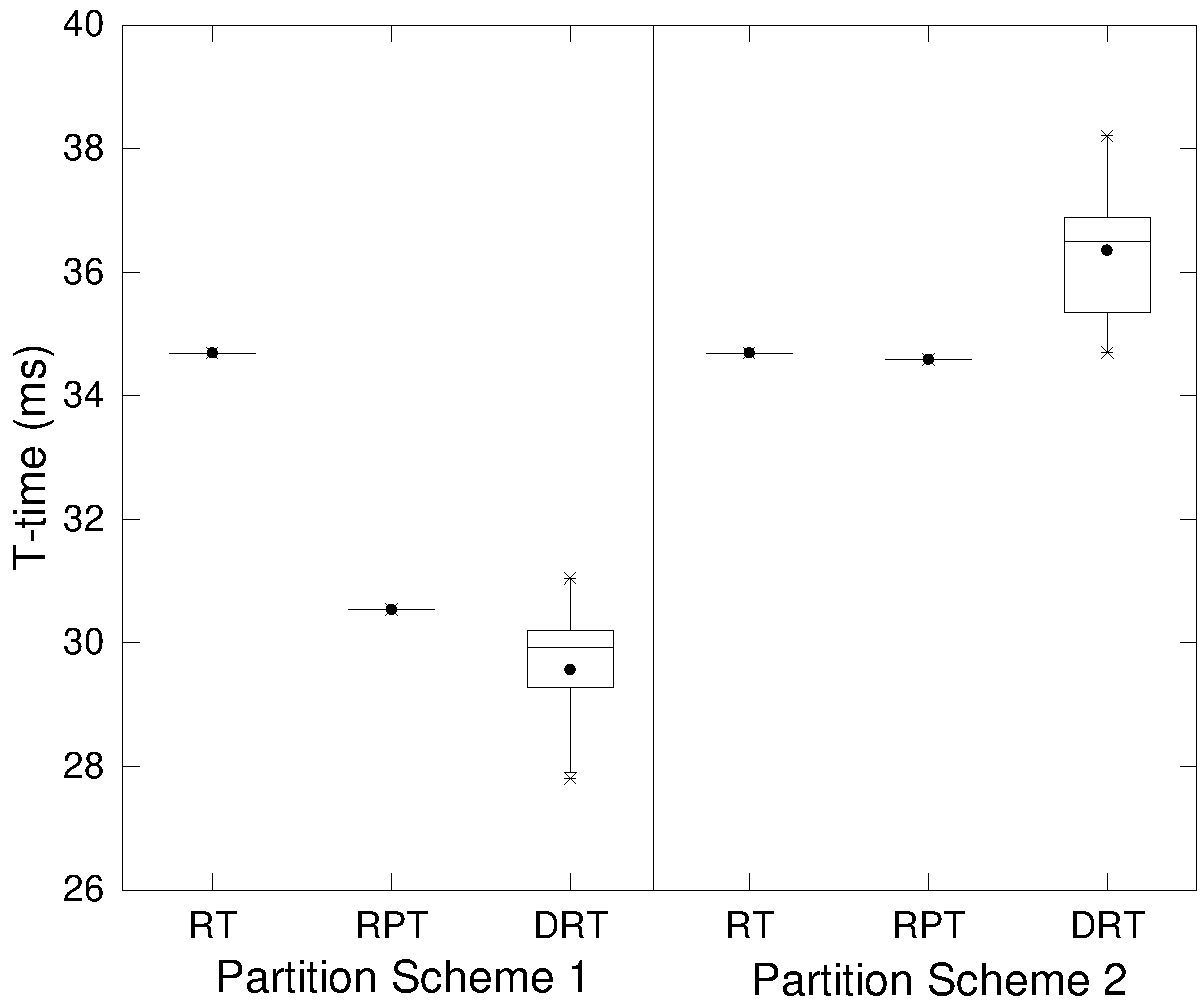
\includegraphics[width=0.32\textwidth,height=4cm]{fig/drttime/chinatimet}}
	\subfigure[PBS] {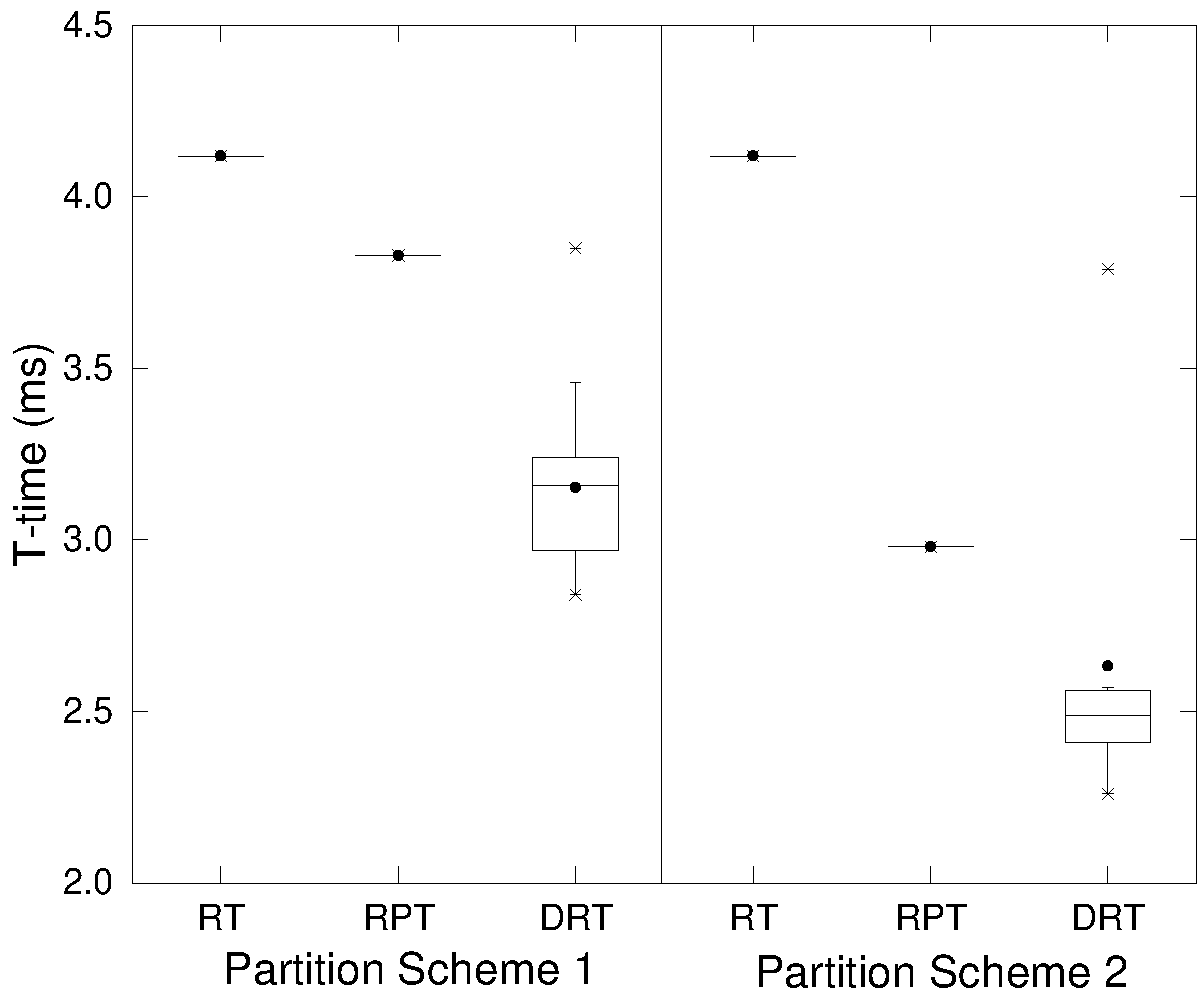
\includegraphics[width=0.32\textwidth,height=4cm]{fig/drttime/parkingtimet}}
	\caption{T-time boxplots for each program}
	\label{fig:Ttime}
\end{figure*}

As was done for the F-, F2-, and T-measure data, we used the Holm-Bonferroni method to check the difference between each pair of testing strategies in terms of F-time, F2-time, and T-time, as shown in Tables~\ref{tableHolm:ftime} to \ref{tableHlom:ttime}.

In Table \ref{tableHlom:ttime}, six entries ("73" \& "3" for DRT vs. RT, "58" vs. "20") are in bold font, meaning that, in terms of T-time, DRT was significantly better than RT, and DRT only marginally outperformed RPT.
Similar observations can be made regarding the F-time and F2-time results.
In other words, the additional computation incurred in DRT by updating the test profile is compensated for in terms of test execution savings.

\begin{table}[!htbp]
  \caption{Number of Scenarios Where The Technique on the Top Row Has a Lower F-time Than That on the Left Column}
  \centering
  \label{tableHolm:ftime}
  \begin{tabular}{|c|c|c|c|} \hline
          &RT         &RPT         &DRT         \\ \hline
    RT    & ---       &5           &\textbf{62} \\ \hline
    RPT   &1          & ---        &\textbf{47} \\ \hline
    DRT   &\textbf{16}&\textbf{31} & ---        \\ \hline
  \end{tabular}
\end{table}

\begin{table}[!htbp]
  \caption{Number of Scenarios Where the Technique on the Top Row Has a Lower F2-time Than That on the Left Column}
  \centering
  \label{tableHlom:nftime}
  \begin{tabular}{|c|c|c|c|} \hline
          &RT         &RPT         &DRT         \\ \hline
    RT    & ---       &3           &\textbf{52} \\ \hline
    RPT   &3          & ---        &\textbf{48} \\ \hline
    DRT   &\textbf{26} &\textbf{30}& ---         \\ \hline
  \end{tabular}
\end{table}

\begin{table}[!htbp]
  \caption{Number of Scenarios Where the Technique on the Top Row Has a Lower T-time Than That on the Left Column}
  \centering
  \label{tableHlom:ttime}
  \begin{tabular}{|c|c|c|c|} \hline
          &RT         &RPT         &DRT         \\ \hline
    RT    & ---       &5           &\textbf{73} \\ \hline
    RPT   &1          & ---        &\textbf{58} \\ \hline
    DRT   &\textbf{3} &\textbf{20} & ---         \\ \hline
  \end{tabular}
\end{table}

It can also be observed from Tables~\ref{tableHolm:ftime} to \ref{tableHlom:ttime} that DRT only slightly outperformed RPT, but that DRT was significantly better than RT, especially in term of $T$-$time$.

In summary, the DRT strategy is considered the best testing technique across all six metrics, and RPT marginally outperformed RT.

\section{Related Work}
\label{sec:relatedwork}

In this section, we describe related work from two perspectives:
related to testing techniques for web services; and
related to improving RT and PT.

\subsection{Testing Techniques for Web Services}

\dpt{I made a lot of changes to this section, please check and confirm}

In recent years, a lot of effort has been made to test web services~\cite{canfora, bozkurt2010, li2014two, felderer2016security}. \dpt{2 references, from 8 and 12 years ago may not be sufficient to support our first sentence here ... }
Test case generation, involving both the generation and selection test cases, is core to testing web services, and model-based~\cite{dalal1999model} and specification-based~\cite{li2009towards} techniques are two common methods. \dpt{no reference for ``specification-based techniques''?}
Before making services available on the Internet, testers can use model-based techniques to verify whether or not the behavior of the WSUT meets their requirements.
In these techniques, test data can be generated from a data model that specifies the inputs to the software---this data model can be built before, or in parallel to, the software development process.
Verification methods using models such as theorem-proving \textcolor{red}{\cite{sinha2006model}}, model-checking \textcolor{red}{\cite{rai2018model}} and Petri-Nets \textcolor{red}{\cite{xiang2015executable}} also exist.
Sinha et al.~\cite{sinha2006model}, for example, used theorem-proving to generate test cases, making use of existing test generation methods based on extended finite state machine (EFSM) specifications.
\textcolor{red}{Zhao et al. \cite{zhao2012model} took advantage of model checking to BPEL script at the logical level, and to generate test cases automatically based on the model description, and finally to select test cases with respect to the counterexamples of model checking output.}
%Majdi et al.~\cite{ghannoudi2015formal} generated test data using model-checking.
\dpt{have we anything else to say about Majdi et al.~\cite{ghannoudi2015formal}?}
%\sout{Dong et al.~\cite{dong2006web} combined high level Petri-Nets (HPN) with constraint-based test data generation obtaining sufficient test data to detect faults.}
\textcolor{red}{Dong et al. \cite{dong2006web} obtained HPN (High-level Petri-Nets) by analyzing WSDL specification. A graph transforming from HPN is used to generate the adapted UIO (unique input output) sequences that presented test cases.}
\dpt{again, this seems a bit lacking in description ... can we say anything more than ``obtaining sufficient test data to detect faults''?}
When testing web services, because it is often only the service's specification that users can receive, specification-based testing is a natural choice.
Typically, the web service specification is contained in the web service description language (WSDL) document, which provides information about the available operations and parameters.
Many methods proposed for WSDL-based test data generation are based on the XML schema data type.
Hanna and Munro proposed a framework that can be used to test the robustness of a web service~\cite{hanna2009approach}.
Their framework analyzes the WSDL documents of web services to identify what faults could impact the robustness, facilitating the design of test cases to detect those faults.

The approaches listed above all aim to generate test cases without consideration of the impact of test case execution order on test efficiency.
In contrast, Bertolino et al.~\cite{bertolino2007automatic} proposed using the category-partition method~\cite{Ostrand88} with XML schemas to perform XML-based partition testing.
Because PT aims to find subsets of all possible test cases to adequately test a system, it can help reduce the required number of test cases.
Our proposed approach involved using software cybernetics with PT:
In DRT, selection of a partition is done according to the testing profile, which is updated throughout the test process.
An advantage of DRT is that partitions with larger failure rates have higher probabilities of selection.
Zhu and Zhang~\cite{zhu2012collaborative} proposed a collaborative testing framework, where test tasks are completed using collaborating test services---a test service is a service assigned to perform a specific testing task.
%Their framework focuses on complete test task.
Our framework (Section~\ref{sec:framework}) aims to find more faults in the WSUT, with the result of the current test case execution providing feedback to the control system so that the next test case selected has a greater chance to reveal faults.

Most existing web service testing techniques assume that the computed output for each test case is verifiable, something that is not always true in practice.
The oracle problem\textcolor{red}{~\cite{barr2015oracle, patel2018mapping}} \rrf refers to those situations where the test case output is not verifiable, and has meant that many testing techniques may not be applicable in some situations.
To address the outstanding oracle problem for testing web services, a metamorphic testing\textcolor{red}{~\cite{chen1998metamorphic,chen2018metamorphic}} \rrf technique has been proposed that not only alleviates the oracle problem, but also presents a feasible and efficient option for testing web services~\cite{sun2011}, \textcolor{red}{in which Sun proposed a metamorphic testing framework for web services and conducted a case study where the framework was employed to test web service. The results of case study showed the feasibility and efficiency of metamorphic testing.}   \dpt{do we want to elaborate a little more on this approach?}

%The proposed DRT for web services has the following advantages: (1) it is easier to use; (2) it is more efficient because it enhances partition testing with dynamic testing profiles updates and the assocaited overhead is very limited. DRT is applicable whenever partition testing is applicable.

\subsection{Improving RT and PT}

Based on the observation that failure causing inputs tend to cluster into contiguous regions within the input domain~\cite{Ammann88, Finelli91}, significant work has been done aiming to improve RT\textcolor{red}{~\cite{cai2009random, chen2010adaptive}}. \rrf
Adaptive random testing~\cite{chen2010adaptive} is a family of advanced techniques based on random testing that aim to improve the failure detection effectiveness by evenly spreading test cases throughout the input domain.
One of the most well-known ART approaches is fixed-size candidate set ART (FSCS-ART)\textcolor{red}{~\cite{chen2001proportional}}, \rrf, but many other ART algorithms have been developed and their effectivenesses validated through simulation and experiments\textcolor{red}{~\cite{chen2010adaptive, barus2016cost, zhang2016test, mao2017out, chen2018test}}.
\dpt{shall we list more? RRT? Linear-order ART? etc?}

Adaptive testing (AT)~\cite{Cai07, hu2009improved} is based on the same observation \textcolor{red}{as ART}\dpt{which observation? same as for ART?}, and has been shown to \sout{outperform both RT and RPT} \textcolor{red}{perform better than RT and RPT in fault detection}. \dpt{outperform in what sense? Failure detection? F-measure? E-/P-measure?}
However, AT may require a very long execution time in practice.
To alleviate this, Cai et al.~\cite{cai2009random} proposed DRT, which uses testing information to dynamically adjust the testing profile.
There are several things that can impact on DRT's test efficiency.
Yang et al.~\cite{Yang2014Dynamic} proposed A-DRT, which adjusts parameters during the testing process.
Li et al.~\cite{li2015} developed O-DRT, which \textcolor{red}{has an objective function and a pre-defined parameter $f$ that is criterion. During the testing process, the value of the objective function is calculated. If this value is greater than $f$, then test profile will be adjusted to a theoretically optimal one.} \sout{changes the testing profile to a theoretically optimal one when a pre-defined criterion is satisfied.} \dpt{can we give an example of the criterion?}
Lv et al.~\cite{Lv2011} studied the relationship of parameters in DRT, but did not give the relationship between parameters and the number of partitions. \dpt{I'm not sure that I understand the intended meaning of the previous sentence. Can you rephrase it?}

\section{Conclusion}
\label{sec:conclusion}

In this paper, to address the challenges of testing SOA-based applications, we have presented a dynamic random testing (DRT) technique for web services.
Our technique uses random testing to generate test cases, and selects test cases for execution from different partitions in accordance with a testing profile that is dynamically updated in response to the test data collected.
In this way, the proposed test technique includes benefits form both random testing and partition testing.

We proposed a framework that examines key issues when applying DRT to testing web services, and developed a prototype to make the method  feasible and effective.
To help guide testers to correctly set the DRT parameters, we used a theoretical analysis to identify the relationships between numbers of partitions, DRT parameters, and the partitions failure rates. \dpt{Please check that I have the correct intended meaning in the previous sentence}
Three real web services were used as experimental objects to validate the feasibility and effectiveness of our approach.
The results of the empirical study show that, in general, DRT obtains better performance than both RT and RPT \textcolor{red}{according to F-, F2-, and T-measure}\dpt{according to what criteria/measures?}, and always \textcolor{red}{have a better}\sout{delivers an outstanding} \dpt{``outstanding''?} \sout{and stable} performance when the DRT parameters \textcolor{red}{setting follow our guidelines }\sout{lie in our theoretically derived interval}.
In other words, our theoretical analysis can provide genuinely useful guidance when DRT is used.

In our future work, we plan to conduct experiments on more web services to further validate its effectiveness, and identify the limitations of our method.

% use section* for acknowledgment
\section*{Acknowledgment}

This research is supported by
the National Natural Science Foundation of China (under Grant No. 61872039),
the Beijing Natural Science Foundation (Grant No. 4162040),
the Aeronautical Science Foundation of China (Grant No. 2016ZD74004), and
the Fundamental Research Funds for the Central Universities (Grant No. FRF-GF-17-B29).

% Can use something like this to put references on a page
% by themselves when using endfloat and the captionsoff option.
\ifCLASSOPTIONcaptionsoff
  \newpage
\fi


\bibliographystyle{IEEEtran}
\bibliography{DRT4WS}
\begin{IEEEbiography}[{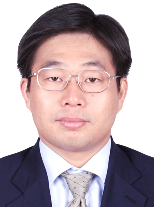
\includegraphics[width=1in,height=1.25in,clip,keepaspectratio]{fig/authors/CASun.pdf}}]{Chang-ai Sun} is a Professor in the School of Computer and Communication Engineering, University of Science and Technology Beijing.
\dpt{Do you want to say anything about what happened between assistant professor at Jiaotong and full professor at USTB?}
Before that, he was an Assistant Professor at Beijing Jiaotong University, China, a postdoctoral fellow at the Swinburne University of Technology, Australia, and a postdoctoral fellow at the University of Groningen, The Netherlands. He received the bachelor degree in Computer Science from the University of Science and Technology Beijing, China, and the PhD degree in Computer Science from the Beihang University, China.
\dpt{Should we say ``Beijing University of Aeronautics and Astronautics, Beijing, China.'' instead of ``Beihang''?}
His research interests include software testing, program analysis, and Service-Oriented Computing.
\end{IEEEbiography}
%\begin{IEEEbiography}[{\includegraphics[width=1in,height=1.25in,clip,keepaspectratio]{YZhao}}]
\begin{IEEEbiography}[{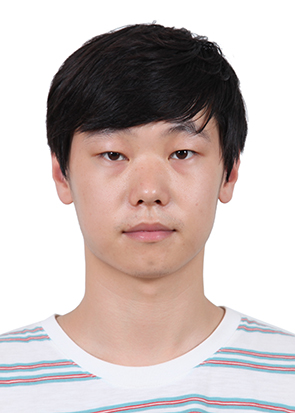
\includegraphics[width=1in,height=1.25in,clip,keepaspectratio]{fig/authors/HPDai.jpg}}]{Hepeng Dai} is a PhD student in the School of Computer and Communication Engineering, University of Science and Technology Beijing, China. He received the master degree in Software Engineering from University of Science and Technology Beijing, China and the bachelor degree in Information and Computing Sciences from China University of Mining and Technology, China. His current research interests include software testing and debugging.
\end{IEEEbiography}
%\begin{IEEEbiography}[{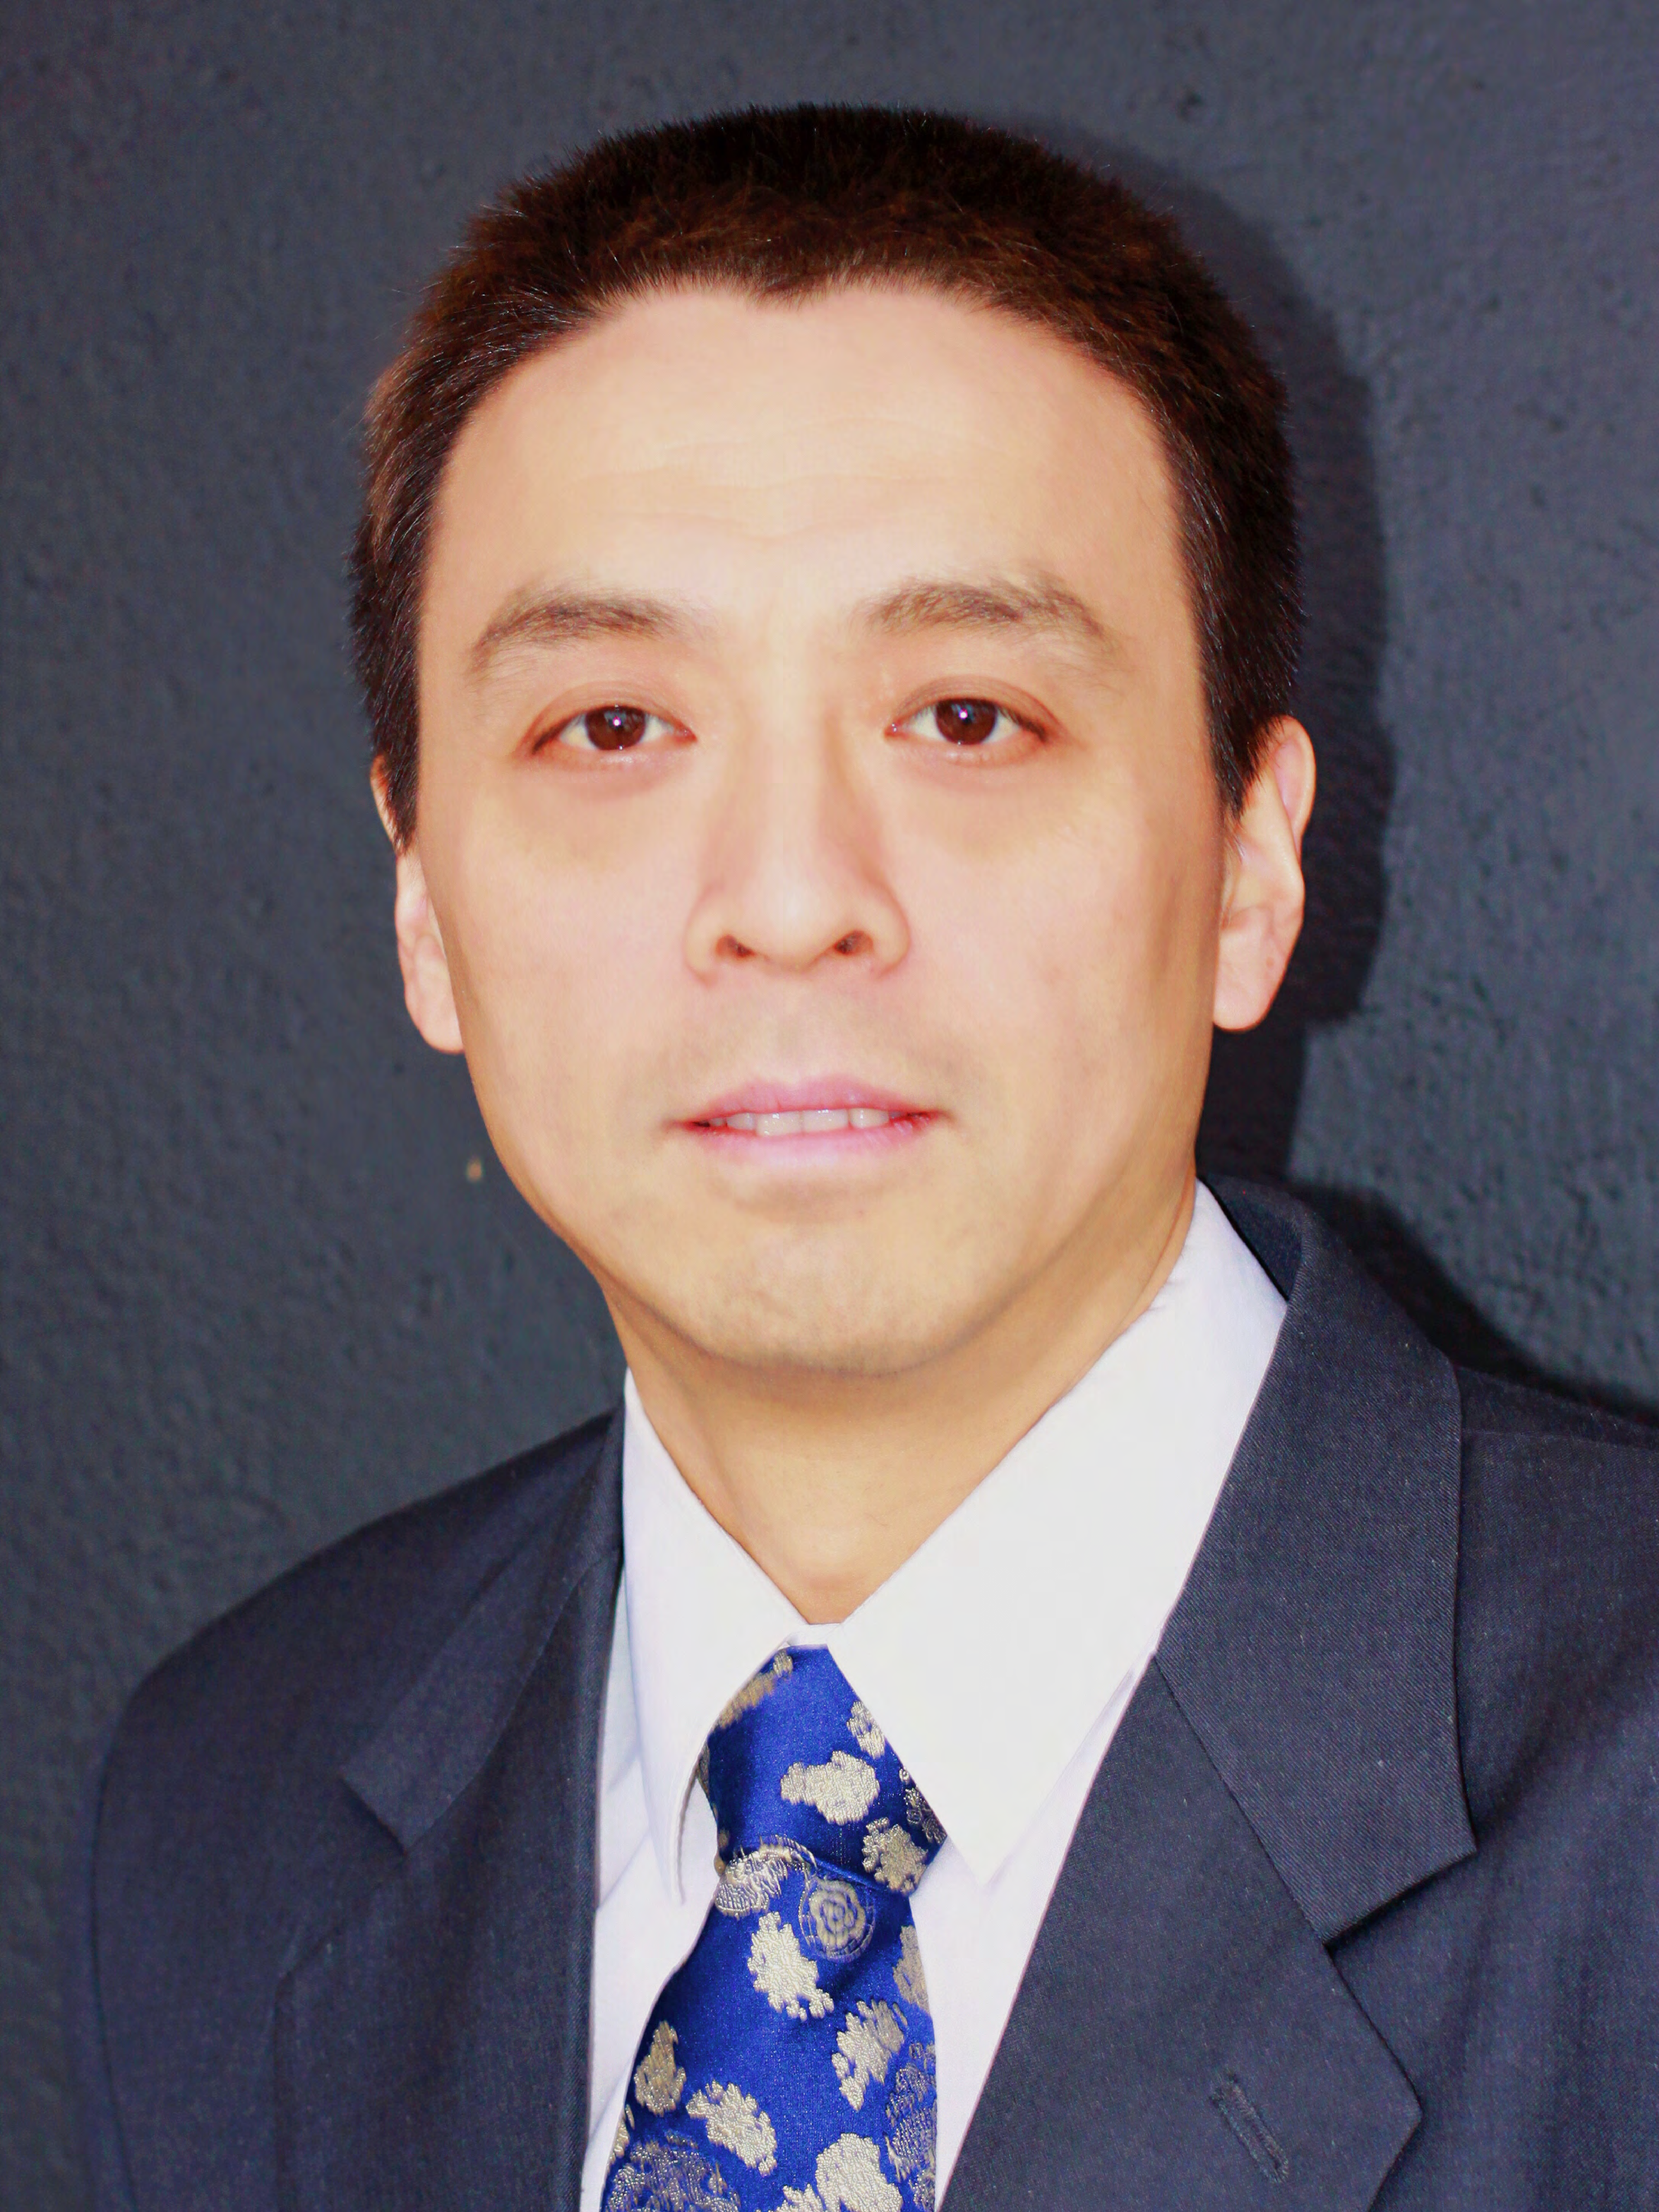
\includegraphics[width=1in,height=1.25in,clip,keepaspectratio]{HLiu}}]
\begin{IEEEbiography}[{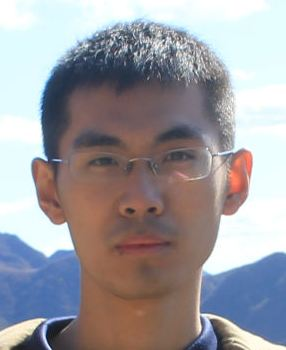
\includegraphics[width=1in,height=1.25in,clip,keepaspectratio]{fig/authors/GWang.jpg}}]{Guan Wang} is a master
\dpt{MSc ?} student at the School of Computer and Communication Engineering, University of Science and Technology Beijing. He received a bachelor degree in Computer Science from University of Science and Technology Beijing. His current research interests include software testing and Service-Oriented Computing.
\end{IEEEbiography}
%\begin{IEEEbiography}[{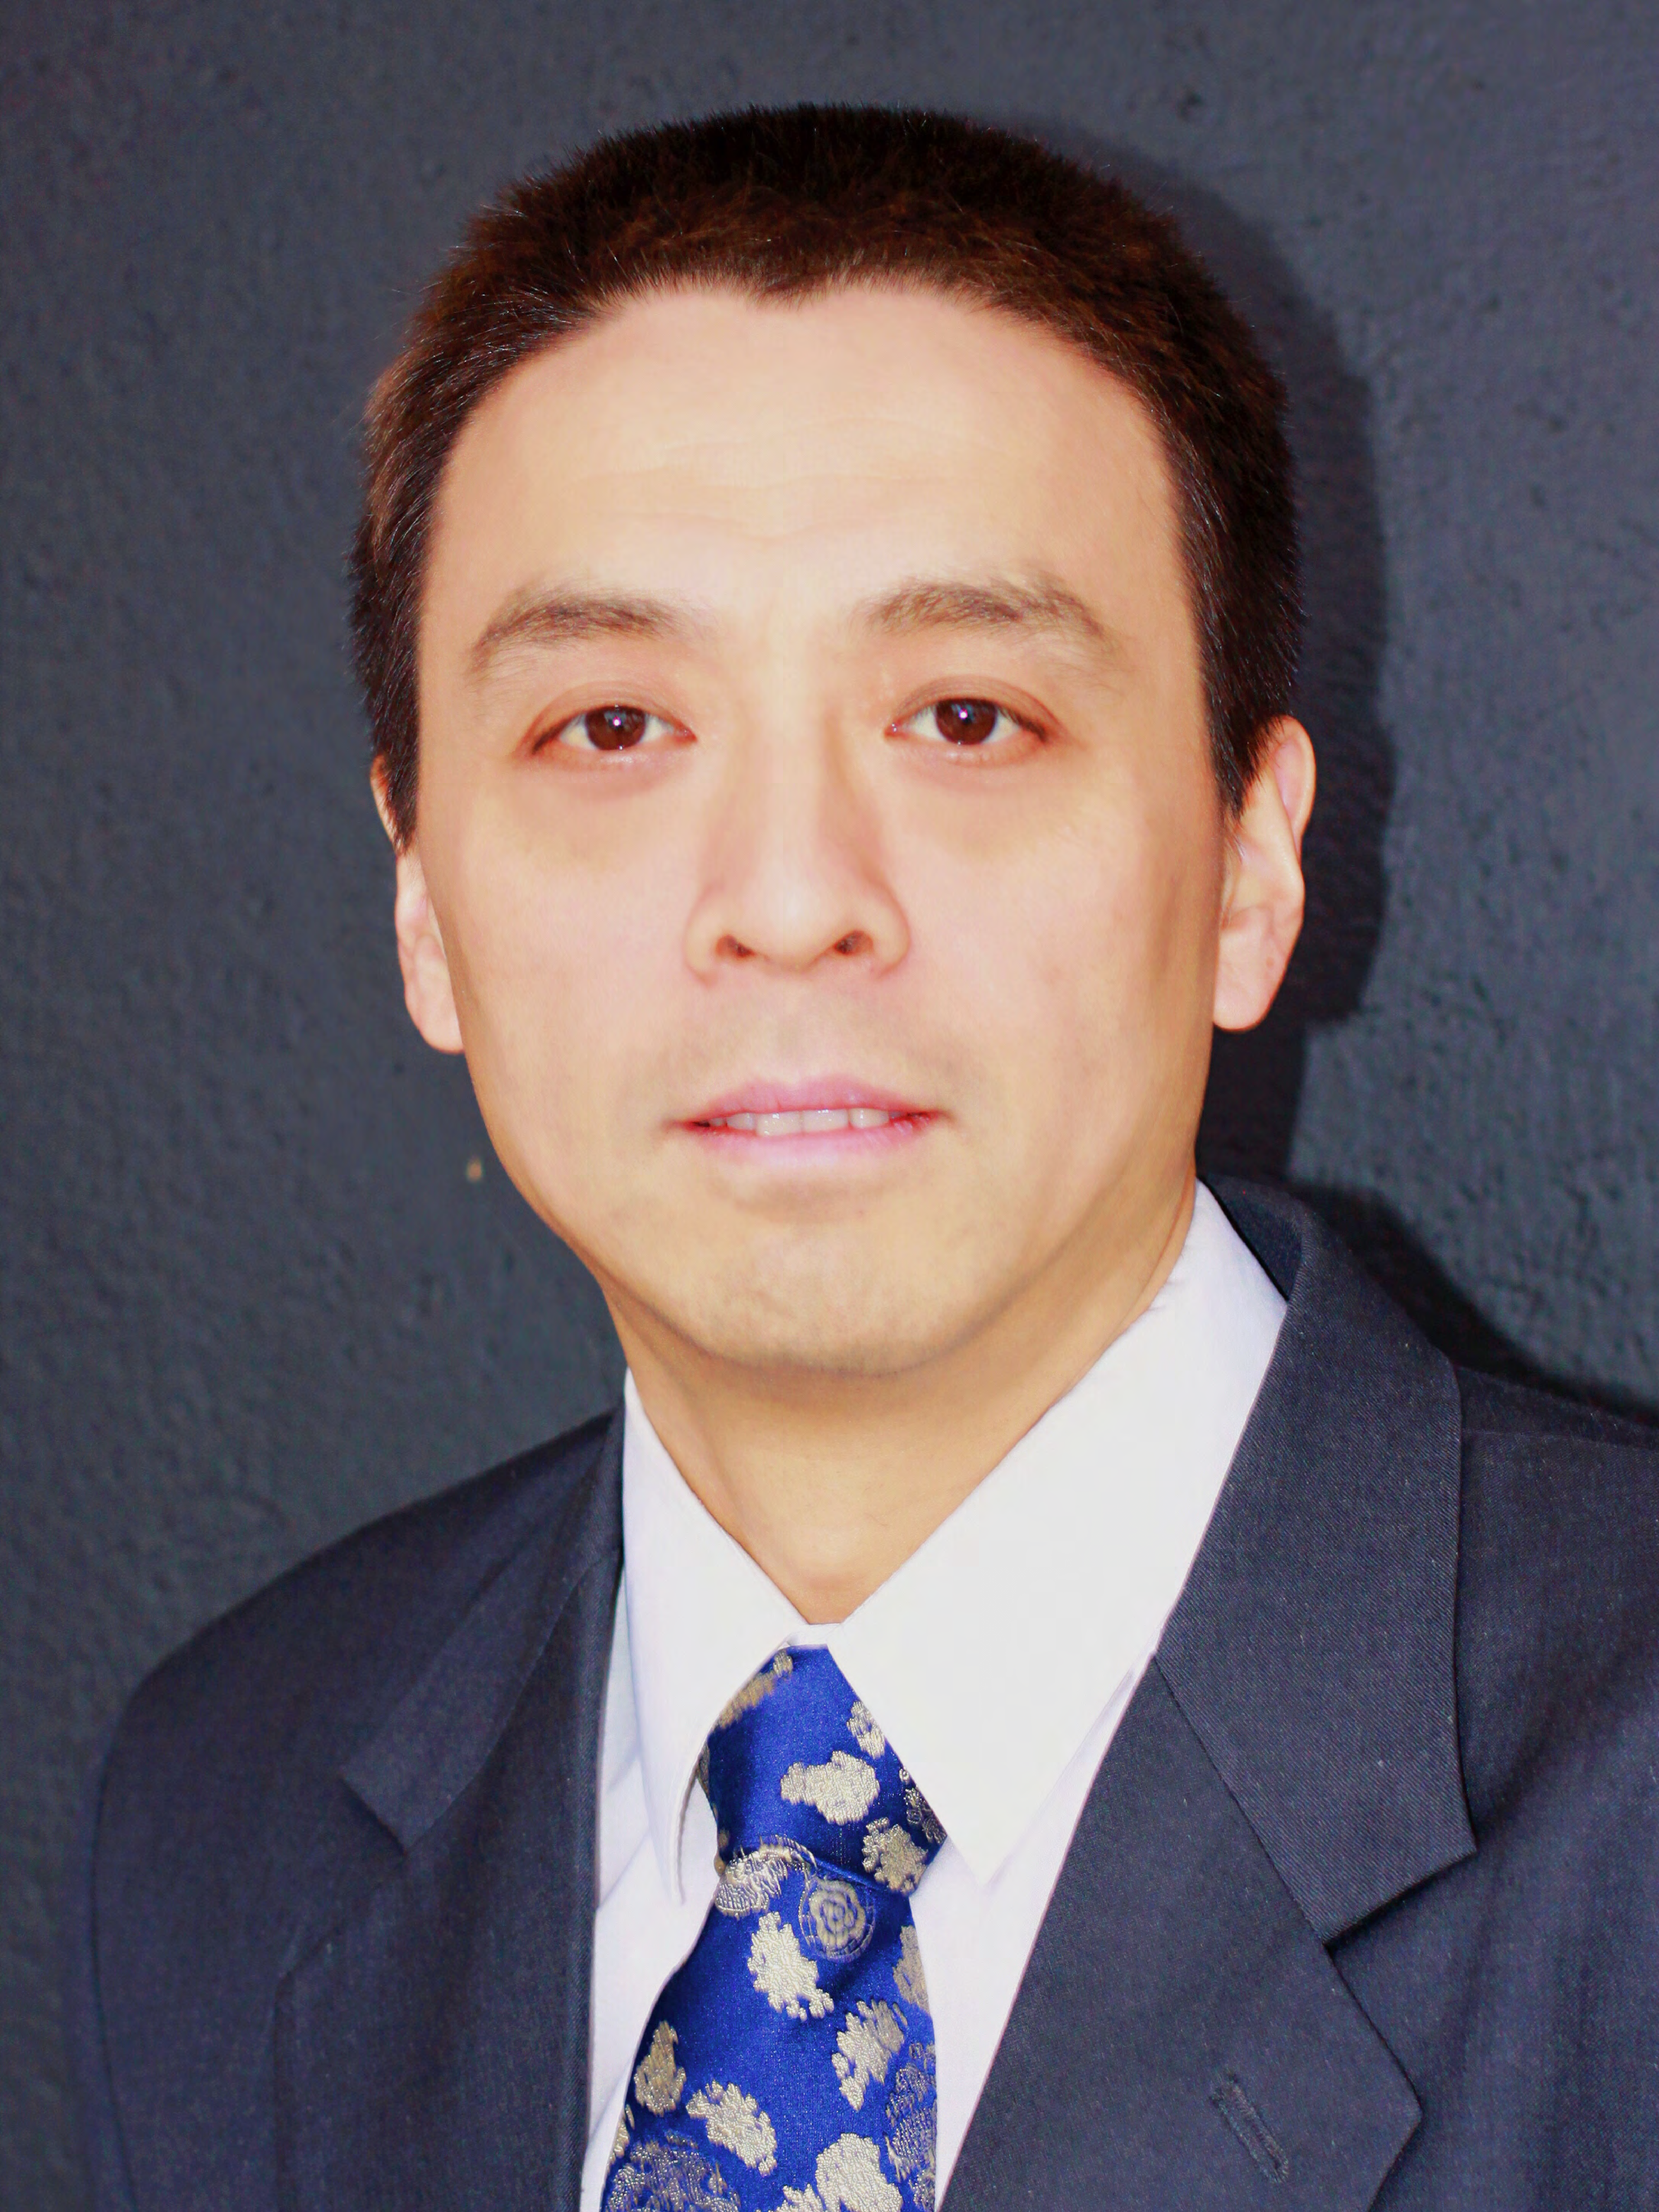
\includegraphics[width=1in,height=1.25in,clip,keepaspectratio]{HLiu}}]
\begin{IEEEbiography}[{
\includegraphics[width=1in,height=1.25in,clip,keepaspectratio]{fig/authors/DaveTowey.png}}]{Dave Towey} is an associate professor in the School of Computer Science, University of Nottingham Ningbo China. He received his BA and MA degrees from The University of Dublin, Trinity College, PgCertTESOL from The Open University of Hong Kong, MEd from The University of Bristol, and PhD from The University of Hong Kong. His current research interests include technology-enhanced teaching and learning, and software testing, especially metamorphic testing and adaptive random testing. He is a  member of both the IEEE and the ACM.
\end{IEEEbiography}
\begin{IEEEbiography}[{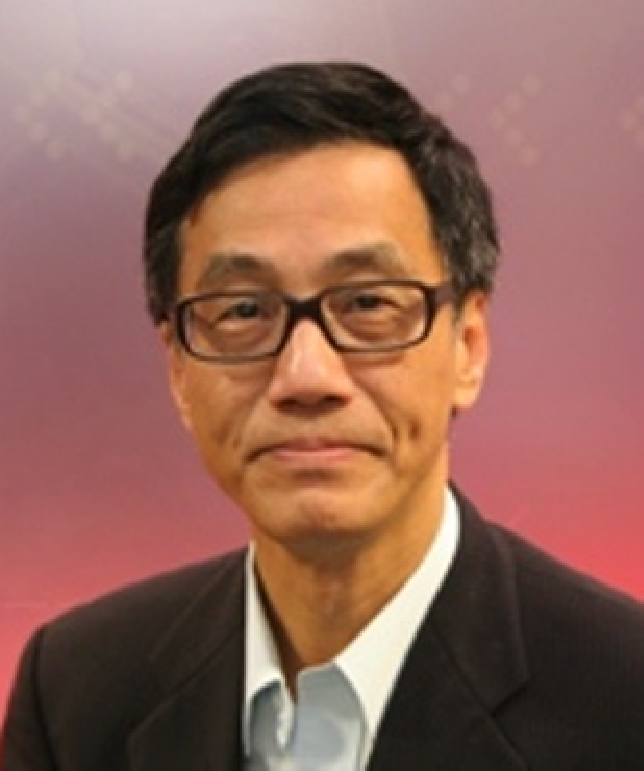
\includegraphics[width=1in,height=1.25in,clip,keepaspectratio]{fig/authors/TYChen.pdf}}]{Tsong Yueh Chen} is a Professor of Software Engineering at the Department of Computer Science and Software Engineering in Swinburne University of Technology. He received his PhD in Computer Science from The University of Melbourne, the MSc and DIC from Imperial College of Science and Technology, and BSc and MPhil from The University of Hong Kong. His current research interests include software testing and debugging, software maintenance, and software design.
\end{IEEEbiography}
%\begin{IEEEbiography}[{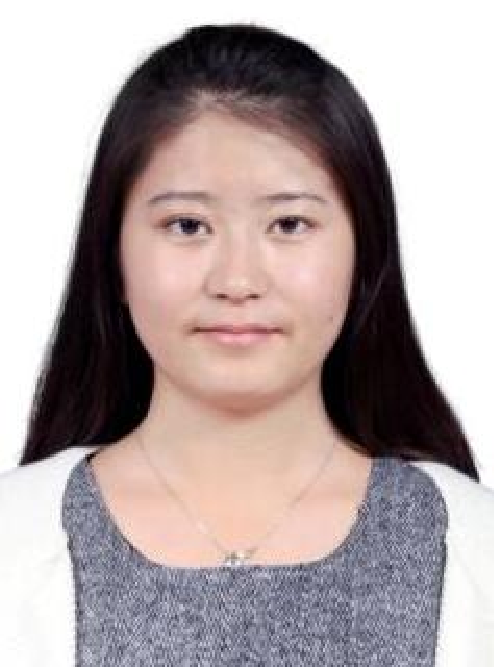
\includegraphics[width=1in,height=1.25in,clip,keepaspectratio]{LPan}}]
\begin{IEEEbiography}[{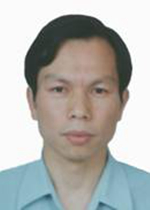
\includegraphics[width=1in,height=1.25in,clip,keepaspectratio]{fig/authors/KYCai.pdf}}]{Kai-Yuan Cai} received the BS, MS, and PhD degrees from \sout{Beijing University of Aeronautics and Astronautics} \textcolor{red}{Beihang university}, Beijing, China, in 1984, 1987, and 1991, respectively. He has been a full professor at Beihang University since 1995.
\dpt{Should we say ``Beijing University of Aeronautics and Astronautics, Beijing, China.'' instead of ``Beihang''?}
He is a Cheung Kong Scholar (chair professor), jointly appointed by the Ministry of Education of China and the Li Ka Shing Foundation of Hong Kong in 1999. His main research interests include software testing, software reliability, reliable flight control, and software cybernatics. \dpt{I've modified this bio slightly, please confirm}
\end{IEEEbiography}


\end{document}
